\documentclass[12pt,a4paper]{report}

% Tabele
\usepackage{longtable}
\usepackage{booktabs}
\usepackage{tabularx}
\usepackage{array}

\usepackage{microtype}
\usepackage{xstring}

\setlength{\emergencystretch}{3em}

% Aby wykresy mogły znajdować się pomiędzy tekstem
\usepackage{float}

% Marginesy - standard 2.5 cm
\usepackage{geometry}
\geometry{margin=2.5cm}

% Interlinia 1,15
\usepackage{setspace}
\setstretch{1.15}

% Język polski
\usepackage{polyglossia}
\setmainlanguage{polish}

% Cudzysłowy itp.
\usepackage{csquotes}

% Czcionki - Times New Roman / Arial
\usepackage{fontspec}
\setmainfont{Times New Roman}
\setsansfont{Arial}
% Kody źródłowe - Consolas (zgodnie z wymaganiami); gdy font nie jest
% zainstalowany w systemie, używamy wizualnie zbliżonego zamiennika,
% aby praca kompilowała się także bez fontów Microsoft.
\IfFontExistsTF{Consolas}
  {\setmonofont{Consolas}}
  {\setmonofont{Courier New}}

% Małe wcięcia dla lepszego wyglądu
\setlength{\parindent}{24pt}

% Drobne przerwy pomiędzy akapitami
\setlength{\parskip}{0.5\baselineskip}

% Matematyka
\usepackage{amsmath}
\usepackage{amssymb}

% Diagramy (TikZ)
\usepackage{tikz}
\usetikzlibrary{positioning,arrows.meta,shapes.geometric,fit,calc,backgrounds,automata}

% Rysunki
\usepackage{graphicx}
\graphicspath{{rysunki/}{wykresy/}}

% Tabele
\usepackage{booktabs}

% Podpisy rysunków i tabel - mała czcionka, wyrównanie do lewej
\usepackage[singlelinecheck=false,justification=raggedright,font=small]{caption}
\addto\captionspolish{
  \renewcommand{\figurename}{Ilustracja}
  \renewcommand{\listfigurename}{Spis ilustracji}
  \renewcommand{\tableautorefname}{Tabela}
  \renewcommand{\figureautorefname}{Ilustracja}
}
\renewcommand{\tablename}{Tabela}
\renewcommand{\listfigurename}{Spis ilustracji}

\usepackage{listings}

% Ustawienia globalne dla dużych bloków (lstinputlisting / begin{lstlisting})
% Te ustawienia dają: ramkę, numery linii, stałą szerokość znaków
\lstset{
  basicstyle=\ttfamily\setstretch{1}\fontsize{9}{10}\selectfont, % Consolas 9pt, interlinia 1
  numbers=left,            % Numery linii po lewej
  numberstyle=\tiny,       % Małe cyferki
  stepnumber=1,            % Numeruj każdą linię
  numbersep=5pt,           % Odstęp numerów
  captionpos=b,            % Podpis pod kodem
  frame=single,            % Ramka
  breaklines=true,         % Łamanie linii
  breakatwhitespace=false, 
  keepspaces=true,
  showstringspaces=false,
  columns=fixed            % W blokach stała szerokość wygląda lepiej (wyrównanie)
}

% Definicja \code{} dla tekstu ciągłego
\newcommand{\code}[1]{%
    \lstinline[%
        basicstyle=\ttfamily,      % Normalna wielkość czcionki (nie small)
        numbers=none,              % Bez numerów linii
        frame=none,                % Bez ramki
        columns=fullflexible,      % Naturalne odstępy w tekście
        breaklines=true,           % Włącz łamanie linii
        breakatwhitespace=false,   % Łam wszędzie
        literate={_}{\_}{1}        % KLUCZOWE: Traktuj _ jako znak, po którym wolno łamać linię
    ]{#1}%
}

\renewcommand{\lstlistingname}{Listing}
\renewcommand{\lstlistlistingname}{Spis listingów}

% Wielopoziomowe nagłówki: 1., 1.1., 1.1.1.
\usepackage[indentafter]{titlesec}  % Dodać wcięcie również w pierwszym akapicie
\titleformat{\chapter}[hang]{\bfseries\Large}{\thechapter.}{1em}{}
\titleformat{\section}[hang]{\bfseries\large}{\thesection}{1em}{}
\titleformat{\subsection}[hang]{\bfseries\normalsize}{\thesubsection}{1em}{}

\setcounter{secnumdepth}{3}
\setcounter{tocdepth}{3}

% Numer strony w prawym dolnym rogu - wszędzie
\usepackage{fancyhdr}

% domyślny styl stron
\pagestyle{fancy}
\fancyhf{}
\fancyfoot[R]{\thepage}
\renewcommand{\headrulewidth}{0pt}

% pierwsze strony rozdziałów, spis treści itd. (styl \enquote{plain})
\fancypagestyle{plain}{%
  \fancyhf{}%
  \fancyfoot[R]{\thepage}%
  \renewcommand{\headrulewidth}{0pt}%
}

% Linki
\usepackage[hidelinks]{hyperref}
\usepackage{xurl}
\renewcommand{\figureautorefname}{Ilustracja}

% Bibliografia - APA (7. edycja)
\usepackage[style=apa,backend=biber]{biblatex}
% biblatex-apa nie ma natywnego pliku polskiego - mapujemy na american-apa
\DeclareLanguageMapping{polish}{american-apa}
\addbibresource{bibliografia.bib}

% Ułatw LaTeX'owi łamanie linków w bibliografii
\setcounter{biburlnumpenalty}{9000}
\setcounter{biburlucpenalty}{9000}
\setcounter{biburllcpenalty}{9000}

% =============================================
% WYCISZANIE OSTRZEŻEŃ (Overfull/Underfull)
% =============================================

% 1. Underfull (zbyt luźne odstępy)
\hbadness=5500      % Wyłącza "Underfull \hbox" (poziome - tekst)
\vbadness=5500      % Wyłącza "Underfull \vbox" (pionowe - strony)

% 2. Overfull (wystawanie poza margines)
\hfuzz=5pt          % Ignoruj wystawanie tekstu o mniej niż 15 punktów
\vfuzz=5pt          % Ignoruj "wystawanie" treści w pionie (np. za długa tabela na stronie)

\begin{document}

% ======================
% STRONA TYTUŁOWA
% ======================
\begin{titlepage}
    \thispagestyle{empty}

    % Logo PJATK - centrowane na górze
    \begin{center}
        
\includegraphics[width=0.8\textwidth]{pjatk-logo.png}
    \end{center}

    \vspace{2.5cm}

    % Nazwa wydziału / katedry / specjalizacji
    \begin{center}
        {\bfseries Programowanie aplikacji biznesowych}\\[1cm]
        {\bfseries Katedra Inżynierii Oprogramowania}\\[0.5cm]
        Wydział Informatyki
    \end{center}

    \vspace{1.5cm}

    % Imię, nazwisko, nr albumu
    \begin{center}
        {\bfseries Jakub Głocki}\\[0.5cm]
        s26523
    \end{center}

    \vspace{0.5cm}

    % Tytuł pracy
    \begin{center}
        {\bfseries\Large Wytworzenie systemu obsługi zamówień z~użyciem technologii chmurowych oraz mikroserwisów}
    \end{center}

    \vspace{2.0cm}

    % Rodzaj pracy + promotor - blok po prawej
    \begin{flushright}
        Praca Inżynierska\\[1cm]
        Promotor:\\
        dr Krzysztof Barteczko
    \end{flushright}

    \vfill

    % Miejsce, miesiąc rok obrony - wyśrodkowane na dole
    \begin{center}
        Warszawa, czerwiec 2026
    \end{center}

\end{titlepage}

% Strona tytułowa bez numeru, numeracja od 2
\setcounter{page}{2}

% ======================
% STRESZCZENIE (PL) - strona 2, poza spisem treści
% ======================
\chapter*{Streszczenie}

Niniejsza praca przedstawia projekt, implementację oraz wdrożenie w~chmurze publicznej kompletnego systemu obsługi
zamówień, zbudowanego w~architekturze mikroserwisowej. System składa się z~trzech mikroserwisów napisanych
w~języku Go --- odpowiedzialnych za~zamówienia, katalog produktów oraz~płatności --- komunikujących się
synchronicznie poprzez~interfejsy REST oraz~asynchronicznie poprzez~zdarzenia domenowe publikowane do~brokera
Apache Kafka, a~także z~aplikacji webowej (Vue~3) stanowiącej interfejs użytkownika. Warstwę danych zrealizowano
na~bazie PostgreSQL, a~uwierzytelnianie --- w~oparciu o~protokół OAuth~2.0 z~rozszerzeniem PKCE i~usługę Amazon
Cognito.

System uruchomiono na~zarządzanym klastrze Kubernetes (Amazon EKS), w~ramach infrastruktury zdefiniowanej
w~całości jako~kod (Terraform), objętej automatyzacją wdrożeń (GitHub Actions) oraz~monitoringiem (Prometheus,
Grafana). Działanie systemu zweryfikowano w~docelowym środowisku chmurowym testami funkcjonalnymi
i~wydajnościowymi; w~teście obciążeniowym system obsłużył kilkaset żądań na~sekundę bez~błędów, automatycznie
skalując liczbę replik. Pracę uzupełniają analiza kosztów utrzymania środowiska oraz~identyfikacja wąskich gardeł
wraz z~rekomendacjami optymalizacji.

\noindent\textbf{Słowa kluczowe:} mikroserwisy, Kubernetes, Amazon Web Services, architektura sterowana
zdarzeniami, infrastruktura jako kod, Go

\clearpage


% ======================
% SPIS TREŚCI
% ======================
\tableofcontents
\clearpage

% ======================
% ROZDZIAŁY - pliki w katalogu \enquote{rozdzialy}
% ======================
\chapter*{Wstęp}
\phantomsection
\addcontentsline{toc}{chapter}{Wstęp}
\label{chap:wstep}

Handel elektroniczny w ostatniej dekadzie stał się jednym z ~najszybciej rozwijających się
obszarów internetu. Systemy zamówień muszą mierzyć się z wieloma wyzwaniami.
Takimi jak zmienne w~czasie obciążenie, jak największa dostępność, krótkie czasy odpowiedzi oraz częstymi zmianami.
Architektura monolityczna w~której cała logika biznesowa zawiera się w~jednej aplikacji okazuje się niewystarczająca.
Zarówno pod względem skalowalności jak i~tempa rozwoju oprogramowania.

Odpowiedzią przemysłu informatycznego na te ograniczenia stała się architektura mikroserwisowa, 
polegająca na dekompozycji systemu na zbiór niewielkich, niezależnie wdrażanych usług, 
z~których każda odpowiada za wyodrębniony fragment domeny biznesowej i~komunikuje się z~pozostałymi 
poprzez dobrze zdefiniowane interfejsy \cite{newman2021}. Podejście to, choć rozwiązuje wiele problemów monolitu, 
wprowadza jednocześnie nowe wyzwania: konieczność zarządzania komunikacją między usługową, zapewnienia spójności 
danych rozproszonych pomiędzy usługami, a~także orkiestracji, monitorowania i~skalowania wielu niezależnych komponentów \cite{richardson2018}. 
W~praktyce przemysłowej wyzwania te adresowane są przy użyciu konteneryzacji, platform orkiestracji, z~spośród 
których standardem de facto stał się Kubernetes \cite{burns2022} oraz usług chmury publicznej, przejmujących 
od zespołów deweloperskich znaczną część odpowiedzialności za utrzymanie infrastruktury.

Niniejsza praca podejmuje się tego zagadnienia w~ujęciu praktycznym. Jej przedmiotem jest budowa kompletnego systemu 
obsługi zamówień zbudowanego. Utworzonego w~architekturze mikroserwisowej i~wdrożonego w~chmurze publicznej Amazon Web Services.
Z~wykorzystaniem zarządzanej usługi Kubernetes (Amazon EKS). Praca ta obejmuje pełny cykl budowy oprogramowania.
Zaczynając od analizy i projektu systemu. Idąc przez implementacje aplikacji webowej i jej backendu. Z wykorzystaniem
infrastruktury chmurowej w~podejściu \emph{infrastructure as code}. Kończąc na testach i analizie działania systemu
w~środowisku docelowym (chmurowym).

\section*{Cel i zakres pracy}
\phantomsection
\addcontentsline{toc}{section}{Cel i zakres pracy}
\label{sec:cel-i-zakres-pracy}

Celem tej pracy jest zaprojektowanie, implementacja oraz wdrożenie w~chmurze Amazon Web Services systemu obsługi
zamówień opartego na architekturze mikroserwisowej. Ponadto praca obejmuje weryfikację
poprawności działania systemu, która zostanie przeprowadzona za pomocą testów manualnych oraz obciążeniowych. Rezultatem tej pracy będzie wykazanie jak za pomocą wymienionych technologii
można wytworzyć relatywnie szybko system z dobrą skalowalnością, obserwowalnością oraz bezpieczeństwem.

Cel główny pracy można rozdzielić na:

\begin{itemize}
    \item teoretyczną analizę podstaw architektury mikroserwisowej oraz związanymi z nią technologiami (konteneryzacja, Kubernetes, usługi chmurowe AWS),
    \item zaprojektowanie modelu domenowego, architektury usług oraz kontraktów komunikacyjnych systemu obsługi zamówień, 
    \item implementację mikroserwisów realizujących obsługę zamówień, katalog produktów oraz proces płatności,
    \item implementację aplikacji webowej stanowiącej interfejs użytkownika systemu,
    \item budowę kompletnego środowiska uruchomieniowego w~chmurze AWS w~podejściu \emph{infrastructure as code},
    \item przeprowadzenie testów systemu oraz analizę jego działania i~kosztów utrzymania w~środowisku chmurowym.
\end{itemize}

Zakres pracy obejmuje wytworzenie następujących komponentów:

\begin{itemize}
    \item trzech mikroserwisów zaimplementowanych w~języku Go: serwisu zamówień (\code{order-service}), serwisu 
    produktów (\code{product-service}) oraz serwisu płatności (\code{payment-service}), komunikujących 
    się synchronicznie poprzez interfejsy REST/JSON oraz asynchronicznie poprzez zdarzenia domenowe publikowane do brokera Apache Kafka,
    \item aplikacji webowej typu SPA (\emph{single-page application}) zbudowanej w~oparciu o~framework Vue~3 i~język TypeScript, 
    umożliwiającej przeglądanie katalogu produktów, składanie zamówień oraz realizację płatności,
    \item warstwy persystencji opartej na relacyjnej bazie danych PostgreSQL, uruchamianej jako zarządzana usługa Amazon RDS,
    \item mechanizmów uwierzytelniania i~autoryzacji użytkowników zrealizowanych z~użyciem usługi Amazon Cognito i~tokenów JWT,
    \item infrastruktury chmurowej zdefiniowanej w~całości w~narzędziu Terraform,
    \item podsystemu monitorowania opartego na narzędziach Prometheus i~Grafana, uruchomionych wewnątrz klastra Kubernetes,
\end{itemize}

Poza zakresem pracy pozostaje implementacja usług pomocniczych jak powiadomienia oraz analityka. Integracja z~rzeczywistymi
operatorami płatności. Wytworzenie procesów ciągłej integracji za pomocą CI/CD zrealizowanych w GitHub Actions.
Tematy te zostaną omówione jedynie jako kierunki dalszego rozwoju systemu w~podsumowaniu pracy. 

\section*{Uzasadnienie wyboru tematu}
\phantomsection
\addcontentsline{toc}{section}{Uzasadnienie wyboru tematu}
\label{sec:uzasadnienie-wyboru-tematu}

Wybór tematu pracy wynika ze~znaczenia omawianych technologii we współczesnym przemyśle informatycznym.

Architektura mikroserwisowa wraz z~konteneryzacją i~orkiestracją przestały być rozwiązaniami niszowymi, 
zarezerwowanymi dla największych firm technologicznych. Badania społeczności Cloud Native Computing Foundation wskazują, 
że zdecydowana większość organizacji wykorzystujących technologie chmurowe stosuje Kubernetes w~środowiskach produkcyjnych, 
a~odsetek ten systematycznie rośnie \cite{cncf2023}. 

System zamówień jest bardzo dobrą dziedziną do wykorzystania architektury mikroserwisowej. Dzieli się ona łatwo na odrębne
tematy biznesowe takie jak: katalog produktów, zamówienia oraz płatności. Pomiędzy nimi występują interakcje synchroniczne
jak i asynchroniczne. Wymusza to zmierzenie się z~kluczowymi problemami systemów rozproszonych.

Literatura obszernie opisuje poszczególne technologie z~osobna, ale ich integracja w~spójny, działający system pozostaje
zadaniem wymagającym praktycznego doświadczenia. Zamiarem tej pracy było zweryfikowanie na rzeczywistym przykładzie, jakie kompromisy
i koszty niesie za sobą uruchomienie takiego systemu w~chmurze publicznej. Udokumentowani

\section*{Przegląd technologii chmurowych w kontekście mikroserwisów}
\phantomsection
\addcontentsline{toc}{section}{Przegląd technologii chmurowych w kontekście mikroserwisów}
\label{sec:przeglad-technologii-chmurowych}

Chmura obliczeniowa definiowana jest jako model umożliwiający wygodny, sieciowy dostęp na żądanie do współdzielonej puli konfigurowalnych 
zasobów obliczeniowych, które mogą być szybko przydzielane i~zwalniane przy minimalnym zaangażowaniu dostawcy \cite{nist2011}.
Można w niej wyróżnić trzy modele usługowe. SaaS (\emph{Software as a~Service}), w~którym produktem jest kompletne oprogramowanie dostępne przez sieć.
IaaS (\emph{Infrastructure as a~Service}), w~którym dostawca udostępnia surowe zasoby obliczeniowe, sieciowe i~dyskowe.
PaaS (\emph{Platform as a~Service}), w~którym udostępniana jest gotowa platforma uruchomieniowa dla aplikacji. Usługi wykorzystane w tej pracy
sytuują się pomiedzy modelami IaaS i~PaaS. Dostawca przyjmuje odpowiedzialność za utrzymanie platformy uruchomieniowej. Pozostawiając
użytkownikowi kontrolę nad jej konfiguracją. Z~perspektywy architektury mikroserwisowej kluczowe znaczenie mają cztery grupy technologii.

Konteneryzacja pozwalająca opakować usługę wraz z~jej zależnościami w~przenośny niezmienny obraz, której standardem de facto stał się Kubernetes: 
platforma automatyzująca rozmieszczanie, skalowanie, samonaprawianie i~aktualizacje kontenerów na klastrze maszyn \cite{burns2022}. 
Wszyscy najwięksi dostawcy chmury publicznej oferują zarządzane warianty Kubernetes.

\emph{infrastructure as code} (IaC), takie jak Terraform, pozwalające opisać całość infrastruktury chmurowej w~postaci deklaratywnego, wersjonowanego kodu.
Podejście to eliminuje ręczną, niepowtarzalną konfigurację środowisk i~umożliwia ich odtworzenie w~sposób w~pełni zautomatyzowany.
Ostatnią grupą są narzędzia wspierające eksploatację systemów rozproszonych. Takie jak systemy monitoringu i~obserwowalności.
Brokery komunikatów umożliwiające asynchroniczną wymianę zdarzeń. CI/CD automatyzujące zmiany w repozytorium i środowisku produkcyjnym.

\section*{Struktura pracy}
\phantomsection
\addcontentsline{toc}{section}{Struktura pracy}
\label{sec:struktura-pracy}

Praca składa się z~jedenastu rozdziałów, które można podzielić na część teoretyczną (rozdziały 1-4), projektową (rozdział 5), 
implementacyjno wdrożeniową (rozdziały 6-9) oraz badawczo-podsumowującą (rozdziały 10-11).

Rozdział~\ref{chap:podstawy-mikroserwisow} przedstawia teoretyczne podstawy architektury mikroserwisowej: porównanie z~architekturą monolityczną, 
modele komunikacji synchronicznej i~asynchronicznej oraz wzorce projektowe stosowane w~systemach rozproszonych. 
Rozdział~\ref{chap:kubernetes} omawia platformę Kubernetes: jej podstawowe obiekty, mechanizmy skalowania, trwałego składowania danych, 
obserwowalności i~bezpieczeństwa. Rozdział~\ref{chap:aws} charakteryzuje chmurę Amazon Web Services oraz usługi wykorzystane w~projekcie, 
wraz z~porównaniem Amazon EKS z~konkurencyjnymi zarządzanymi usługami Kubernetes.

Rozdział~\ref{chap:projekt-systemu} zawiera projekt systemu obsługi zamówień: opis funkcjonalny, model domenowy, architekturę usług, 
projekt interfejsów REST i~kontraktów zdarzeń, a~także uzasadnienie wyboru technologii implementacyjnych. 
Rozdziały~\ref{chap:implementacja-mikroserwisow} i~\ref{chap:implementacja-portalu} opisują implementację odpowiednio mikroserwisów 
backendowych oraz webowego portalu obsługi zamówień. Rozdział~\ref{chap:infrastruktura} przedstawia budowę kompletnego środowiska 
chmurowego w~podejściu \emph{infrastructure as code}.

Rozdział~\ref{chap:testy-i-analiza} poświęcony jest testom systemu oraz analizie jego działania w~środowisku docelowym, 
w~tym analizie kosztów wykorzystania usług chmurowych i~identyfikacji wąskich gardeł. Pracę zamyka rozdział~\enquote{\nameref{chap:wnioski}},
zawierający ocenę stopnia realizacji postawionych celów, omówienie napotkanych trudności oraz rekomendacje dotyczące dalszego rozwoju systemu.

\chapter{Teoretyczne podstawy architektury mikroserwisowej}
\label{chap:podstawy-mikroserwisow}

Rozdział ten przedstawia teoretyczne podstawy architektury mikroserwisowej. Omówiono w~nim różnice
pomiędzy architekturą monolityczną a~mikroserwisową, kluczowe cechy mikroserwisów, modele komunikacji międzyusługowej, a~także wzorce projektowe
stosowane w~systemach rozproszonych. Rozdział zamyka omówienie konteneryzacji oraz roli orkiestracji,
stanowiące wprowadzenie do rozdziału~\ref{chap:kubernetes}.

\section{Architektura monolityczna a mikroserwisowa}
\label{sec:monolit-a-mikroserwisy}

Architektura monolityczna to model budowy aplikacji, w której całość logiki biznesowej kompiluje się i wdraża jako
pojedynczą jednostkę uruchomieniową. Model ten ma istotne zalety. Jest on prosty koncepcyjnie. Transakcje mogą być
lokalne i obejmować cały stan aplikacji. Uproszczone jest testowanie i debugowanie, a~wdrożenie sprowadza się do uruchomienia 
jednego artefaktu. Z~tych powodów monolit pozostaje racjonalnym wyborem dla małych zespołów i~systemów 
o~ograniczonej złożoności \cite{newman2021}.

Problemy architektury monolitycznej ujawniają się wraz z rozbudową systemu i~organizacji. Skalowanie możliwe
jest poprzez dodanie zasobów lub powielenie całej aplikacji. Nawet jeśli wąskim gardłem jest pojedynczy moduł.
Każda zmiana wymaga zbudowania i wdrożenia całej aplikacji. Co wydłuża cykl wydawniczy i~zwiększa ryzyko regresji.
Brak wymuszenia granic pomiędzy modułami może powodować z czasem erozje, prowadząc do silnego sprzężenia kodu.
Finalnie cały system związany jest jedną technologią i~jedną wersją zależności, a~awaria dowolnego fragmentu 
może unieruchomić aplikację w~całości \cite{richardson2018}.

Architektura mikroserwisowa stanowi odpowiedź na te ograniczenia. Lewis i~Fowler definiują ją jako podejście,
w~którym pojedyncza aplikacja budowana jest jako zbiór niewielkich usług. Każda działa we własnym procesie
i~komunikuje się z~pozostałymi za pomocą lekkich mechanizmów. Usługi zbudowane są wokół zdolności biznesowych
i~wdrażane niezależnie w~sposób w~pełni zautomatyzowany \cite{fowler2014}. Zestawienie najważniejszych różnic
pomiędzy oboma podejściami przedstawia tabela~\ref{tab:monolit-vs-mikroserwisy}.

\begin{table}[H]
    \centering
    \caption{Porównanie architektury monolitycznej i mikroserwisowej 
    (opracowanie własne na podstawie \cite{newman2021,richardson2018})}
    \label{tab:monolit-vs-mikroserwisy}
    \renewcommand{\arraystretch}{1.25}
    \setlength{\tabcolsep}{8pt}

    \begin{tabularx}{\textwidth}{>{\raggedright\arraybackslash\bfseries}p{3.4cm}
                                    >{\raggedright\arraybackslash}X
                                    >{\raggedright\arraybackslash}X}
        \toprule
        \textbf{Kryterium} 
        & \textbf{Architektura monolityczna} 
        & \textbf{Architektura mikroserwisowa} \\
        \midrule

        Jednostka wdrożenia 
        & Cała aplikacja wdrażana jako jedna całość 
        & Pojedyncza, niezależna usługa \\

        Skalowanie 
        & Skalowanie całej aplikacji, nawet gdy obciążony jest tylko jeden moduł 
        & Skalowanie niezależne, dostosowane do potrzeb konkretnej usługi \\

        Baza danych 
        & Najczęściej jedna wspólna baza danych 
        & Odrębna baza danych lub schemat danych dla każdej usługi \\

        Komunikacja wewnętrzna 
        & Bezpośrednie wywołania funkcji lub metod w ramach jednej aplikacji 
        & Komunikacja sieciowa, np. REST, komunikaty lub zdarzenia \\

        Spójność danych 
        & Zwykle zapewniana przez transakcje ACID 
        & Często oparta na spójności ostatecznej \\

        Dobór technologii 
        & Zazwyczaj jednolity stos technologiczny 
        & Możliwość niezależnego doboru technologii dla poszczególnych usług \\

        Izolacja awarii 
        & Ograniczona; awaria jednego modułu może wpływać na całą aplikację 
        & Większa; awaria może zostać ograniczona do pojedynczej usługi \\

        Złożoność operacyjna 
        & Relatywnie niska, prostsze wdrażanie i monitorowanie 
        & Wysoka, wymaga orkiestracji, monitoringu i zarządzania komunikacją \\

        Cykl wydawniczy 
        & Wspólny dla całej aplikacji, zwykle mniej elastyczny 
        & Niezależny dla poszczególnych usług, umożliwiający częstsze wdrożenia \\

        \bottomrule
    \end{tabularx}
\end{table}

Należy podkreślić, że mikroserwisy nie są rozwiązaniem uniwersalnie lepszym. Przenoszą one złożoność z~wnętrza aplikacji
do przestrzeni pomiędzy usługami. Takimi jak sieć, infrastruktura czy procesy wdrożeniowe. Wybór tej architektury jest
uzasadniony wówczas, gdy gdy korzyści z~niezależnego skalowania i~wdrażania przewyższają koszt zwiększonej
złożoności operacyjnej. Z tych powodów praktyczna realizacja mikroserwisów jest bardzo związana z~technologiami
chmurowymi i~ich automatyzacją.

\section{Charakterystyka mikroserwisów}
\label{sec:charakterystyka-mikroserwisow}

Literatura przedmiotu \cite{newman2021,richardson2018} wskazuje zestaw cech konstytuujących architekturę
mikroserwisową, które można sprowadzić do następujących zasad.

\textbf{Modelowanie wokół domeny biznesowej.} Granice usług powinny odpowiadać granicom kontekstów biznesowych
(\emph{bounded contexts}) w~rozumieniu projektowania sterowanego domeną (\emph{Domain-Driven Design}) \cite{evans2003}.
Usługa bierze odpowiedzialność za wyodrębniony fragment domeny. W realizowanym systemie te fragmenty to:
zamówienia, katalog produktów oraz płatności. Minimalizuje to liczbę zmian wymaganych do koordynacji między
usługami.

\textbf{Niezależność wdrożeniowa.} Każda usługa może być zbudowana, przetestowana i~wdrożona bez udziału pozostałych. 
Separacja ta pozwala rozwijać i testować aplikacje samodzielnie. Wymaga to jawnych wersjonowanych kontraktów komunikacyjnych 
oraz unikanie współdzielenia struktur danych. Bardzo dobrą praktyką jest rozdzielenie struktur na komunikacyjną i transportową.

\textbf{Ukrywanie informacji i~własność danych.} Usługa udostępnia na zewnątrz wyłącznie swój interfejs, ukrywając
szczegóły implementacji. Konsekwencją jest zasada \emph{database-per-service}. Każda usługa jest wyłącznym właścicielem swoich danych.
Inne usługi mogą uzyskać do nich dostęp jedynie poprzez jej interfejs. Złamanie tej zasady prowadzi do sprzężenia na poziomie schematu, 
które w~praktyce odbiera usługom niezależność wdrożeniową \cite{newman2021}.

\textbf{Decentralizacja i~autonomia technologiczna.} Usługi mogą być rozwijane przez niezależne zespoły 
i~realizowane w~różnych technologiach, dobranych do charakteru problemu.

\textbf{Odporność na awarie.} W systemie rozproszonym awarie są normalnym zjawiskiem. Architektura musi zakładać że usługi 
mogą być chwilowo niedostępne. Ograniczenie takich awarii można osiągnąć poprzez asynchroniczną komunikacje oraz samonaprawiające się usługi.

\textbf{Obserwowalność.} Zachowanie systemu rozproszonego wymaga dokładnego monitorowania, ponieważ każda usługa działa całkowicie oddzielnie.
Wymagane jest dokładne monitorowanie każdej z nich w celu wykrywania anomalii. Niezbędne więc staje się gromadzenie metryk,
logów i informacji o stanie każdej usługi. Zagadnienie to rozwinięto w~rozdziale~\ref{chap:kubernetes}
oraz, w~odniesieniu do implementacji, w~rozdziale~\ref{chap:implementacja-mikroserwisow}.

\section{Komunikacja synchroniczna i asynchroniczna}
\label{sec:komunikacja-synchroniczna-asynchroniczna}

Dekompozycja systemu na usługi czyni z~komunikacji międzyusługowej zagadnienie architektonicznie pierwszorzędne.
Wyróżnia się dwa zasadnicze modele tej komunikacji, różniące się sprzężeniem czasowym pomiędzy stronami.

\subsection{Komunikacja synchroniczna - REST}
\label{subsec:komunikacja-synchroniczna}

W~modelu synchronicznym usługa wywołująca wysyła żądanie i~wstrzymuje przetwarzanie do czasu otrzymania odpowiedzi.
Najpowszechniejszą realizacją tego modelu są interfejsy REST (\emph{Representational State Transfer}) oparte na
protokole HTTP i~formacie JSON. Zasoby identyfikowane są za pomocą adresów URL, a~operacje metodami HTTP (GET, POST, PUT, DELETE).
Zaletami podejścia jest prostota, łatwość testowania oraz zgodność z~modelem żądanie-odpowiedź.
Podobnym dla interakcji użytkownika z serwisem.

Wadą komunikacji synchronicznej jest sprzężenie czasowe. Obie strony muszą być dostępne jednocześnie, a~niedostępność
lub spowolnienie usługi wywoływanej propaguje się na wywołującą. W~łańcuchach wywołań prowadzi to do awarii
kaskadowych, w~których problem jednej usługi unieruchamia kolejne \cite{richardson2018}. Powoduje to złamanie paradygmatu
mikroserwisów czyli odporność na awarie. Z~tego względu komunikacje synchroniczną stosuje się głównie na styku użytkownik-system.

\subsection{Komunikacja asynchroniczna i architektura sterowana zdarzeniami}
\label{subsec:komunikacja-asynchroniczna}

W~modelu asynchronicznym nadawca przekazuje komunikat pośrednikowi brokerowi komunikatów i~natychmiast
kontynuuje przetwarzanie, nie oczekując na odbiorców. Szczególną postacią tego modelu jest architektura sterowana
zdarzeniami (\emph{event-driven architecture}), w~której usługi publikują zdarzenia domenowe. Niemutowalne fakty
opisujące to, co zaszło w~ich obszarze odpowiedzialności (np. \emph{utworzono zamówienie}). Subskrybeńci 
pobierają te zdarzenia i obsługują je według własnej logiki. Dzięki temu rozszczepieniu serwisów, nadawca nie zna swoich
odbiorców. Powoduje to łatwe dodawanie kolejnych subskrybentów bez zmian po stronie producenta \cite{kleppmann2017}.

Model ten eliminuje sprzężenie czasowe. Chwilowa niedostępność konsumenta nie wpływa na producenta.
Wiadomości nieprzetworzone będą czekały w systemie kolejkowym do ponownego działania subskrybenta. 
Ceną jest rezygnacja z~natychmiastowej, silnej spójności danych na rzecz spójności ostatecznej (\emph{eventual consistency}).
Stan rozproszony pomiędzy usługami mże być obsłużony z opóźnieniem, co system musi uwzględniać w finalnej architekturze.
Istotne są również gwarancje dostarczania. Brokery komunikatów typowo zapewniają dostarczenie \emph{co najmniej raz}, co oznacza, że ten
sam komunikat może zostać doręczony wielokrotnie. Konsumenci muszą zatem przetwarzać komunikaty w~sposób idempotentny \cite{kleppmann2017}.

W~zrealizowanym systemie oba modele zastosowano komplementarnie: żądania użytkownika obsługiwane są synchronicznie
przez REST. Natomiast proces walidacji zamówienia i~rezerwacji stanów magazynowych przebiega asynchronicznie, poprzez
zdarzenia publikowane do brokera Apache Kafka. Szczegóły tego podziału omówiono w~rozdziale~\ref{chap:projekt-systemu}.

\section{Wzorce projektowe w systemach mikroserwisowych}
\label{sec:wzorce-projektowe}

Problemy powtarzające się w~systemach mikroserwisowych doczekały się skatalogowanych rozwiązań (wzorców
projektowych) \cite{richardson2018}. Poniżej omówiono wzorce, które znalazły bezpośrednie zastosowanie
w~zrealizowanym systemie; odwołania do ich implementacji zawiera rozdział~\ref{chap:implementacja-mikroserwisow}.

\textbf{Baza danych na usługę (\emph{database-per-service}).} Każda usługa posiada wyłączność na swoje dane
i~udostępnia je jedynie poprzez interfejs. Wzorzec ten został zaimplementowany tylko częściowo gdzie 
serwis zamówień nie dotyka danych produktowych i płatniczych. Wysyłając asynchronicznie żądanie o rezerwację
produktów.

\textbf{Zdarzenia domenowe i~choreografia.} Proces biznesowy obejmujący wiele usług. Może być koordynowany
centralnie (orkiestracja) lub być realizowany jako łańcuch reakcji na zdarzenia (choreografia). Każda usługa,
przetworzywszy swój etap, publikuje zdarzenie, na które reagują kolejne. W~zrealizowanym systemie cykl walidacji
zamówienia przebiega według choreografii. Serwis zamówień publikuje zdarzenie utworzenia zamówienia, na które
serwis produktów odpowiada rezerwacją stanów magazynowych i~publikacją wyniku walidacji.

\textbf{Idempotentny odbiorca i~klucz idempotencji.} Komunikaty mogą docierać wielokrotnie, a~klient może
ponowić żądanie (np. po utracie odpowiedzi w~sieci). Operacje zmieniające stan muszą być odporne na powtórzenia.
Realizuje się to poprzez klucz idempotencji. Jest ot unikalny identyfikator operacji przekazywany przez klienta i zapamiętywany przez usługę.
Dzięki tej logice powtórne żądanie nie tworzy duplikatu, a zwraca wynik już wykonanej operacji.


\textbf{Maszyna stanów.} Cykl życia encji biznesowej w~omawianym systemie zamówienia modelowany jest jako
skończony automat stanów. Z~jawnie zdefiniowanym zbiorem dozwolonych przejść. Wzorzec ten uniemożliwia wprowadzenie
encji w~stan niespójny (np. opłacenie zamówienia anulowanego) i~porządkuje logikę biznesową wokół przejść pomiędzy
stanami.

\textbf{Brama API i~odwrócone proxy.} Klient systemu nie komunikuje się z~usługami bezpośrednio. Istnieje pojedynczy 
punkt wejścia, który przekierowuje żądania do odpowiednich serwisów na podstawie ścieżki. Upraszcza to konfiguracje 
klientów. Pozwala uniknąć CORS. Ukrywa wewnętrzną topologię systemu.

\textbf{Konfiguracja zewnętrzna.} Zgodnie z~metodyką \emph{The Twelve-Factor App} konfiguracja zależna od środowiska
(adresy usług, poświadczenia, przełączniki funkcji) przechowywana jest poza kodem. W~zmiennych środowiskowych.
Dzięki czemu ten sam artefakt może być wdrażany w~różnych środowiskach bez rekompilacji \cite{twelvefactor}.

\textbf{Kontrola zdrowia (\emph{health check}).} Każda usługa udostępnia punkt końcowy raportujący jej stan.
Odpytywany jest przez platformę uruchomieniową w~celu wykrywania niezdrowych instancji. Zapobiega to awarii
przez automatyczny ich restart lub wyłączenie z~puli.

\section{Konteneryzacja i rola orkiestracji}
\label{sec:konteneryzacja-i-orkiestracja}

Praktyczna realizacja architektury mikroserwisowej wymaga jednolitego sposobu pakowania i~uruchamiania wielu
niezależnych usług. Rolę tę pełni konteneryzacja. Jest to technika wirtualizacji na poziomie systemu operacyjnego.
Procesy izolowane są od siebie przy użyciu jądra Linux, współdzieląc przy tym jądro systemu gospodarza.
W~odróżnieniu od maszyn wirtualnych kontenery nie wymagają odrębnego systemu operacyjnego, dzięki czemu 
uruchamiają się w~ułamkach sekund i~wprowadzają znikomy narzut wydajnościowy \cite{burns2022}.

Jednostką dystrybucji jest obraz kontenera. Niemutowalny, warstwowy artefakt zawierający aplikację wraz z~kompletem
jej zależności, budowany na podstawie deklaratywnego opisu (\emph{Dockerfile}). Przchowywany jest on w~rejestrze
obrazów. Niemutowalność obrazu zapewnia powtarzalność wdrożeń. Eliminuje to błędy wynikające z~różnic z~środowiskami.

Konteneryzacja rozwiązuje problem pojedynczej usługi. Jednak nie odpowiada na pytania jak: na którym węźle uruchomić kontener?, jak utrzymać zadaną liczbę jego replik mimo awarii
węzłów?, jak kierować ruch do zmieniających się dynamicznie instancji?, jak przeprowadzić aktualizację bez przerwy w działaniu?, jak skalować liczbę replik w odpowiedzi na obciążenie.
Zadania te są określane jako orkiestracja kontenerów. Wymaga to specjalnej platformy której standardem stał się Kubernetes, któremu poświęcono następny rozdział.
\chapter{Kubernetes jako platforma uruchomieniowa mikroserwisów}
\label{chap:kubernetes}

Kubernetes jest otwartoźródłową platformą orkiestracji kontenerów, automatyzującą ich rozmieszczanie, skalowanie
i~eksploatację na klastrze maszyn. Projekt, zainicjowany przez firmę Google w~2014 roku i~czerpiący z~jej
wieloletnich doświadczeń z~wewnętrznym systemem Borg, został przekazany fundacji Cloud Native Computing Foundation
i~stał się standardem przemysłowym w~obszarze orkiestracji \cite{burns2022}.

U~podstaw działania Kubernetes leży model deklaratywny. Użytownik zamiast wydawać platformie poleceń, opisuje
pożądany stan systemu (np. \emph{trzy repliki usługi zamówień w~wersji 1.2}). Platforma ciągle porównuje stan
faktyczny z~pożądanym. Przy różnicach niweluje rozbieżności (pętla uzgadniania, \emph{reconciliation loop}).
Z takiego modelu wynika samonaprawialność systemu. Awaria jakiegoś kontenera, węzła czy usługi powoduje rozbieżność
którą platforma próbuje usunąć.

Architektura klastra Kubernetes obejmuje płaszczyznę sterowania (\emph{control plane}), serwer API, magazyn
stanu etcd, planistę (\emph{scheduler}) oraz menedżery kontrolerów. Obejmuje również węzły robocze (\emph{worker nodes}),
na których agent \emph{kubelet} uruchamia kontenery zgodnie z~decyzjami planisty \cite{k8sdocs}. Taka architektura
pozwala usługom chmurowym wziąć odpwiedzialność za płaszczyznę sterwania. Dzięki czemu użytkownik zarządza wyłącznie
wezłami roboczymi i~uruchamianymi obciążeniami (rozdział~\ref{chap:aws}).

\section{Podstawowe obiekty Kubernetes}
\label{sec:podstawowe-obiekty-kubernetes}

Stan klastra opisywany jest za pomocą obiektów API. Poniżej omówiono obiekty wykorzystane w~zrealizowanym systemie;
ich konkretne definicje przedstawiono w~rozdziale~\ref{chap:infrastruktura}.

\textbf{Pod} jest najmniejszą jednostką wdrożeniową. Grupą jednego lub kilku kontenerów współdzielących przestrzeń
sieciową (wspólny adres IP) i~woluminy. Najczęściej w praktyce zwiera jeden kontener aplikacyjny. Pody są ulotne,
czyli w każdej chwili mogą zostać usunięte i odtworzone w innym miejscu (węźle). Dzieje się tak np podczas balansowania
gdzie Kubernetes próbuje zmieścić nowe Pody podczas wdrożenia. Wiąże się to z tym że jeśli aplikacja wymaga utrzymania stanu
to musi ją trzymać w zewnętrznym miejscu jak baza danych.

\textbf{Deployment} deklaruje pożądaną liczbę replik poda wraz z~szablonem jego specyfikacji i~strategią
aktualizacji. Za pośrednictwem obiektu ReplicaSet utrzymuje zadaną liczbę replik. Przy zmianie szablonu (np.
nowej wersji obrazu) przeprowadza aktualizację kroczącą (\emph{rolling update}). Nowe repliki uruchamiane są
stopniowo, równolegle z~wygaszaniem starych. Pozwala to wdrażać zmiany bez przerwy w~dostępności usługi.
W~zrealizowanym systemie każdy z~trzech mikroserwisów opisany jest własnym Deploymentem.

\textbf{Service} rozwiązuje problem ulotności podów, udostępniając stabilny, wirtualny punkt dostępu (nazwę DNS
i~adres IP) dla dynamicznie zmieniającego się zbioru replik, wraz z~równoważeniem obciążenia pomiędzy nimi.
Wariant ClusterIP udostępnia usługę wewnątrz klastra, NodePort --- na stałym porcie każdego węzła (wariant ten
wykorzystano do wystawienia ruchu z~zewnętrznego load balancera), a~LoadBalancer zleca utworzenie zewnętrznego
balancera dostawcy chmury.

\textbf{Namespace} dzieli klaster na logiczne przestrzenie nazw, izolując zasoby różnych zespołów lub systemów
i~stanowiąc granicę dla uprawnień oraz limitów zasobów. Komponenty zrealizowanego systemu działają w~dedykowanej
przestrzeni \code{order-portal}.

\textbf{ConfigMap i~Secret} przechowują konfigurację oddzieloną od obrazów kontenerów. ConfigMap zawiere jawną,
a~secret pofuną. Udostępniają one podom zmienne środowiskowe lub pliki. Obiekty te są infrastrukturalną realizacją 
wzorca konfiguracji zewnętrznej (sekcja~\ref{sec:wzorce-projektowe}).

\section{Zarządzanie konfiguracją i skalowaniem}
\label{sec:konfiguracja-i-skalowanie}

Specyfikacja każdego kontenera może określać zapotrzebowanie na zasoby w~postaci żądań (\emph{requests}) i~limitów
(\emph{limits}) dla procesora i~pamięci. Żądania stanowią podstawę decyzji planisty --- pod zostanie umieszczony
wyłącznie na węźle dysponującym wolnymi zasobami w~zadeklarowanej wielkości --- natomiast limity wyznaczają górną
granicę zużycia, której przekroczenie skutkuje dławieniem procesora lub zakończeniem procesu w~przypadku pamięci.
Poprawne określenie tych wartości ma szczególne znaczenie na węzłach o~małej pojemności, jakie wykorzystano
w~środowisku zrealizowanego systemu.

W specyfikacji każdego kontenera należy określić zapotrzebowanie na zasoby. Występuję one w postaci żądań (\emph{requests})
i~limitów (\emph{limits}) dla procesora i~pamięci. Na podstawie żądań planista rozmieszcza pody w węzłach
dysponującymi wolnymi zasobami w zadeklarowanej wielkości. Limity natmiast wyznaczają górną granicę zużycia, której 
przekroczenie powoduje dławieniem procesora lub zakończeniem procesu w przypadku pamięci.
Poprawne określenie tych wartości ma szczególne znaczenie na węzłach o~małej pojemności, jakie wykorzystano
w~środowisku zrealizowanego systemu.

Konfiguracja aplikacji dostarczana jest podom ze źródeł zewnętrznych. Obiektów ConfigMap i~Secret. 
W~zrealizowanym systemie poświadczenia bazy danych trafiają do podów jako zmienne środowiskowe z~obiektów Secret, 
zasilanych z~usługi AWS Secrets Manager (rozdział~\ref{chap:infrastruktura}).

Skalowanie obciążeń realizowane jest na dwóch poziomach. Poziomy pierwszy stanowi \textbf{Horizontal Pod Autoscaler}
(HPA). Kontroler, który cyklicznie porównuje zmierzone wykorzystanie zasobów (domyślnie procesora, na podstawie
danych z~komponentu \emph{metrics-server}). Z~wartością docelową i~odpowiednio zwiększa lub zmniejsza liczbę replik
Deploymentu w~zadanym przedziale \cite{k8sdocs}. Poziom drugi to skalowanie samego klastra, czyli liczby węzłów
roboczych.

\section{Trwałe składowanie danych}
\label{sec:trwale-skladowanie-danych}

System plików kontenera jest ulotny --- ginie wraz z~jego restartem --- a~pody mogą być przenoszone pomiędzy
węzłami, co czyni przechowywanie danych na dysku węzła zawodnym. Kubernetes rozwiązuje ten problem warstwą
abstrakcji nad pamięcią trwałą, rozdzielającą perspektywę administratora i~aplikacji \cite{k8sdocs}.

Zgodnie z definicją Poda, system plików kontenera jest ulotny. Pody mogą być przenoszone między węzłami.
Z tego powdu Kubernetes rozwiązuje ten problem warstwą abstrakcji nad pamięcią trwałą, 
rozdzielającą perspektywę administratora i~aplikacji \cite{k8sdocs}.

\textbf{PersistentVolume} (PV) reprezentuje fizyczny zasób pamięci --- np. wolumin blokowy dostawcy chmury ---
natomiast \textbf{PersistentVolumeClaim} (PVC) jest żądaniem aplikacji: deklaracją potrzebnej pojemności i~trybu
dostępu, niezależną od tego, skąd zasób pochodzi. \textbf{StorageClass} opisuje klasę pamięci (typ nośnika,
parametry wydajnościowe) i~umożliwia provisionowanie dynamiczne: wolumin tworzony jest automatycznie w~chwili
pojawienia się żądania, bez ręcznego przygotowywania zasobów przez administratora. Tworzeniem i~dołączaniem
woluminów zarządza sterownik zgodny ze standardem CSI (\emph{Container Storage Interface}), specyficzny dla danego
dostawcy infrastruktury.

\textbf{PersistentVolume} (PV) reprezentuje fizyczny zasób pamięci. Natomiast \textbf{PersistentVolumeClaim} (PVC) 
jest żądaniem zapotrzebowania aplikacja na taki woluminu o potrzebnej pojemności i~trybu dos†ępu.
\textbf{StorageClass} opisuje klasę pamięci (typ nośnika,parametry wydajnościowe) i~umożliwia provisionowanie dynamiczne.
Wolumin tworzony jest automatycznie w~chwili pojawienia się żądania. Tworzeniem i~dołączaniem
woluminów zarządza sterownik zgodny ze standardem CSI (\emph{Container Storage Interface}), specyficzny dla danego
dostawcy infrastruktury.

W~zrealizowanym systemie pamięci trwałej wymagają broker Kafka oraz serwer Prometheus. Wykorzystano sterownik
AWS EBS CSI z~klasą pamięci opartą na woluminach gp3, skonfigurowaną z~trybem wiązania
\emph{WaitForFirstConsumer}. Wolumin tworzony jest dopiero po zaplanowaniu poda na konkretnym węźle, co
gwarantuje jego utworzenie w~tej samej strefie dostępności, w~której działa pod. Główna baza danych systemu
pozostaje natomiast poza klastrem, jako zarządzana usługa Amazon RDS. Uzasadnienie tej decyzji przedstawiono
w~rozdziale~\ref{chap:aws}.

\section{Obserwowalność: Prometheus i Grafana}
\label{sec:obserwowalnosc-prometheus-grafana}

Obserwowalność systemu rozproszonego opiera się na trzech filarach: metrykach (liczbowych szeregach czasowych
opisujących stan systemu), logach (zapisach zdarzeń) oraz śladach rozproszonych (zapisach przebiegu pojedynczych
żądań przez kolejne usługi). W~zrealizowanym systemie zastosowano dwa pierwsze filary, z~metrykami gromadzonymi
przez Prometheus \cite{prometheusdocs}.

Prometheus działa w~modelu \emph{pull}. Aplikacje wystawiają punkty końcowe z metrykami, które cyklicznie pobiera.
Zbiór celów nie jest konfigurowany statycznie, a w~środowisku Kubernetes Prometheus odkrywa je dynamicznie poprzez API klastra.
O objęciu poda monitoringiem decydują jego adnotacje (\code{prometheus.io/scrape}, \code{prometheus.io/port}).
ozwiązanie to wykorzystano w~zrealizowanym systemie: każdy mikroserwis opatrzony jest adnotacjami wskazującymi 
port techniczny, na którym udostępnia metryki.

Metryki przyjmują postać nazwanych szeregów czasowych z~etykietami (\emph{labels}), umożliwiającymi agregację
i~filtrowanie np. liczba żądań HTTP w~podziale na ścieżkę i~kod odpowiedzi. Typowe rodzaje metryk to liczniki
(\emph{counters}), mierniki (\emph{gauges}) oraz histogramy, pozwalające szacować percentyle czasów odpowiedzi.
Zapytania do zgromadzonych danych formułowane są w~języku PromQL, który umożliwia m.in. wyznaczanie szybkości
zmian liczników czy agregacje po etykietach.

Warstwę prezentacji stanowi Grafana --- narzędzie wizualizacji, które na podstawie zapytań PromQL buduje
interaktywne kokpity (\emph{dashboards}) prezentujące stan systemu w~czasie rzeczywistym i~historycznie. W~obu
narzędziach konfigurację (źródła danych, definicje kokpitów) można dostarczać deklaratywnie, co w~zrealizowanym
systemie wykorzystano do provisionowania Grafany z~poziomu kodu infrastruktury (rozdział~\ref{chap:infrastruktura}).
Zakres metryk publikowanych przez poszczególne mikroserwisy --- w~tym metryk domenowych, takich jak liczba
utworzonych zamówień --- omówiono w~rozdziale~\ref{chap:implementacja-mikroserwisow}.

Warstwę prezentacji stanowi Grafana --- narzędzie wizualizacji, które na podstawie zapytań PromQL buduje
interaktywne kokpity (\emph{dashboards}) prezentujące stan systemu w~czasie rzeczywistym i~historycznie.
Zakres metryk publikowanych przez poszczególne mikroserwisy omówiono w~rozdziale~\ref{chap:implementacja-mikroserwisow}.

\section{Mechanizmy bezpieczeństwa w Kubernetes}
\label{sec:bezpieczenstwo-kubernetes}

Bezpieczeństwo klastra Kubernetes obejmuje kilka współdziałających warstw \cite{k8sdocs}.

\textbf{Uwierzytelnianie i~autoryzacja dostępu do API.} Każde żądanie do serwera API podlega uwierzytelnieniu,
a~następnie autoryzacji w~modelu RBAC (\emph{Role-Based Access Control}): role definiują zestawy dozwolonych
operacji na zasobach, a~powiązania ról (\emph{role bindings}) przypisują je użytkownikom lub kontom usług.
Procesy działające w~klastrze występują wobec API jako \textbf{ServiceAccount} --- konta usług o~jawnie nadawanych,
minimalnych uprawnieniach. W~zrealizowanym systemie własne konto usługi z~ograniczoną rolą posiada serwer
Prometheus, któremu do dynamicznego odkrywania celów pomiarowych wystarczą uprawnienia tylko do odczytu metadanych
podów.

Każde żądanie do serwera API pdlega uwierzytelnieniu i~autoryzacji w~mdelu RBAC (\emph{Role-Based Access Control}).
Role definiują zestawy dozwolonych operacji na zasobach. Powiązania ról (\emph{role bindings}) przypisują je użytkownikom lub kontom usług.
Procesy działające w~klastrze występują wobec API jako \textbf{ServiceAccount}. Konta usług o~jawnie nadawanych,
minimalnych uprawnieniach. W~zrealizowanym systemie własne konto usługi z~ograniczoną rolą posiada serwer
Prometheus. Psiada uprawnienia do dynamicznego odkrywania celów poprzez odczyt metadanych podów.

\textbf{Ochrona danych poufnych.} Obiekty Secret oddzielają poświadczenia od obrazów i~manifestów aplikacji,
a~dostęp do nich podlega RBAC. W~zrealizowanym systemie źródłem poświadczeń bazy danych jest AWS Secrets Manager.

\textbf{Kontekst bezpieczeństwa podów.} Specyfikacja \emph{securityContext} pozwala wymusić uruchamianie procesów
bez uprawnień administratora (\emph{nonroot}). Komplementarną praktyką jest minimalizacja samych obrazów. 
Obrazy klasy \emph{distroless} pozbawione są powłoki i~menedżera pakietów, redukują powierzchnię ataku kontenera.
Podejście to zastosowano dla wszystkich mikroserwisów systemu (rozdział~\ref{chap:implementacja-mikroserwisow}).

\textbf{Segmentacja sieci.} Domyślnie komunikacja pomiędzy podami w~klastrze jest nieograniczona. Obiekty
NetworkPolicy pozwalają zawęzić ją do jawnie dozwolonych przepływów. W~zrealizowanym systemie segmentację ruchu
zrealizowano przede wszystkim na poziomie infrastruktury chmurowej. Grup bezpieczeństwa i~topologii podsieci
(rozdział~\ref{chap:infrastruktura}).

\textbf{Integracja z~systemem uprawnień chmury.} W~środowiskach zarządzanych pody często wymagają dostępu do usług
dostawcy chmury (np. tworzenia woluminów EBS). Zamiast statycznych kluczy stosuje się mechanizmy wiążące konta
usług Kubernetes z~rolami IAM --- w~EKS są to IRSA (\emph{IAM Roles for Service Accounts}) oraz nowszy mechanizm
EKS Pod Identity, który w~zrealizowanym systemie nadaje uprawnienia sterownikowi EBS CSI. Proces otrzymuje wówczas
poświadczenia krótkoterminowe, automatycznie rotowane, o~zakresie ograniczonym do przypisanej roli.

\textbf{Integracja z~systemem uprawnień chmury.} W~środowiskach zarządzanych pody często wymagają dostępu do usług
dostawcy chmury. Wiąże się wtedy konta usług Kubernetes z rolami dostawcy. W~zrealizowanym systemie użyty został
EKS Pod Identity, który nadaje uprawnienia sterownikowi EBS CSI.

Omówione mechanizmy stanowią fundament, na którym zbudowano środowisko uruchomieniowe systemu. Sposób ich
praktycznego użycia  przedstawiono w~rozdziałach~\ref{chap:aws} i~\ref{chap:infrastruktura}.
\chapter{Amazon Web Services jako środowisko chmurowe}
\label{chap:aws}

Amazon Web Services (AWS) jest największą pod względem udziału w~rynku platformą chmury publicznej, oferującą
kilkaset usług. Od surowych zasobów obliczeniowych, przez zarządzane bazy danych i~platformy kontenerowe, po
wyspecjalizowane usługi analityczne. Rozdział ten charakteryzuje platformę AWS oraz omawia usługi, z~których
zbudowano środowisko uruchomieniowe zrealizowanego systemu, a~kończy się porównaniem Amazon EKS z~konkurencyjnymi
zarządzanymi usługami Kubernetes.

\section{Charakterystyka AWS i jego architektury globalnej}
\label{sec:charakterystyka-aws}

Infrastruktura AWS jest podzielona na \textbf{regiony}. Są to geograficznie odseparowane lokalizacje (np. \code{eu-central-1} we Frankfurcie).
Każdy z~nich jest oddzielną domeną awarii i~osobnym miejscem przechowywania danych. Każdy region składa się
z~co najmniej trzech \textbf{stref dostępności} (\emph{Availability Zones}, AZ). Są to fizycznie rozdzielone 
centra danych o~niezależnym zasilaniu i łączności. Połączone są one ze sobą łączami o~niskich opóźnieniach.
Rozmieszczenie komponentów systemu w~wielu strefach dostępności jest podstawową techniką zapewniania
wysokiej dostępności. Awaria pojedynczej strefy nie przerywa działania systemu \cite{awsdocs}.

Model rozliczeń AWS ma wiele form. W podstawowej wersji opłaty naliczane są za faktyczne zużycie zasobów
(czas działania instancji, pojemność, transfer danych). Bez zobowiązań wstępnych. W tym projekcie wykorzystana
została pula bezpłatnych zasobów (\emph{Free Tier}), udostępniona czasowo dla nowych kont. Z tego powodu
wiele decyzji co do doboru parametrów środowiska została podjęta w zakresie bezpłatnego poziomu.

Istotnym elementem charakterystyki platformy jest \textbf{model odpowiedzialności współdzielonej} (\emph{shared
responsibility model}). AWS odpowiada za bezpieczeństwo \emph{samej chmury}. Czyli infrastruktury fizycznej, hipernadzorcy,
oprogramowania usług zarządzanych. Natomiast klient za bezpieczeństwo \emph{w~chmurze}. Czyli konfigurację sieci
i~uprawnień, ochronę danych oraz poprawność własnych aplikacji \cite{awsdocs}.

\section{Amazon EKS - zarządzana usługa Kubernetes}
\label{sec:amazon-eks}

Amazon Elastic Kubernetes Service (EKS) udostępnia klaster Kubernetes. Płaszczyzna sterowania jest w~całości
zarządzana przez AWS. Użytkownik widzi tylko punkt końcowy API \cite{awsdocs}. Użytkownik odpowiada
za dobór wezłów roboczych oraz uruchomienie obciążenia. EKS wykorzystuje niezmodyfikowaną, certyfikowaną 
dystrybucję Kubernetes, dzięki czemu obciążenia i~manifesty pozostają przenośne pomiędzy środowiskami.

Warstwę obliczeniową klastra EKS można zrealizować na dwa sposoby. Jako samodzielnie zarządzane instancje EC2
\textbf{zarządzane grupy węzłów} (\emph{managed node groups}). W~których AWS automatyzuje provisionowanie,
aktualizacje i~wymianę instancji EC2. AWS Fargate, model bezserwerowy, w~którym pojedyncze pody
uruchamiane są bez jawnie widocznych węzłów. W~zrealizowanym systemie wybrano zarządzane grupy węzłów: w~odróżnieniu
od Fargate zachowują one pełną kontrolę nad typem instancji.

Integralną częścią EKS są \textbf{dodatki} (\emph{add-ons}). Zarządzane przez AWS komponenty systemowe klastra.
Przykładem takiej wtyczki może być sieciowa VPC CNI. Przydziela ona podom adresy IP bezpośrednio z~puli
adresowej sieci VPC. Bez niej liczba podów na węźle jest ograniczona liczbą interfejsów sieciowych instancji.
W tym projekcie użyłem małych instancji co stanowiło bariere przy wdrożeniu wszystkich komponentów.

Tożsamość i~dostęp do klastra EKS realizowane są poprzez integrację z~systemem IAM. Zarówno administratorzy, jak
i~węzły robocze uwierzytelniają się wobec API Kubernetes przy użyciu tożsamości IAM (sekcja~\ref{sec:bezpieczenstwo-kubernetes}).

\section{Usługi powiązane wykorzystane w projekcie}
\label{sec:uslugi-powiazane}

\subsection{Amazon EC2 jako warstwa obliczeniowa}
\label{subsec:ec2}

Amazon Elastic Compute Cloud (EC2) dostarcza maszyny wirtualne (\emph{instancje}). Mają one zróżnicowane zasoby
opisane typami instancji. W zrealizowanym systemie użyte zostały jako węzły EKS. Stanowią one warstwę obliczeniową klastra.
W celu zmieszczenia w darmowym programie użyte zostały instancje \code{t3.small} w~trybie \emph{on-demand}.
Grupa węzłów posiada konfigurowalny przedział wielkości (minimalna, pożądana i~maksymalna liczba instancji). 
Stanowi to infrastrukturalny fundament skalowania klastra.

\subsection{Amazon RDS for PostgreSQL jako warstwa danych}
\label{subsec:rds}

Amazon Relational Database Service (RDS) jest zarządzaną usługą relacyjnych baz danych, przejmującą od użytkownika
instalację, łatanie, kopie zapasowe i~odtwarzanie silnika bazodanowego. W~realizowanym systemie użyto RDS PosgreSQL.
Korzystają z~niej wszystkie 3 mikroserwisy. Instancja umieszczona jest w~podsieci prywatnej. Z~grupą bezpieczeństwa,
która umożliwia dostęp tylko z sieci klastra. Decyzja użycia RDS zamiast bazy uruchamianej w~klastrze, wynika
z~dostarczenia wszystkich potrzebnych mechanizmów dla bazy produkcyjnej przez serwis.

\subsection{Amazon ECR - rejestr obrazów kontenerów}
\label{subsec:ecr}

Amazon Elastic Container Registry (ECR) jest prywatnym rejestrem obrazów kontenerów, zintegrowanym z~systemem
uprawnień IAM. W~zrealizowanym systemie utworzono po jednym repozytorium dla każdego mikroserwisu, z~włączonym
automatycznym skanowaniem obrazów pod kątem znanych podatności oraz polityką cyklu życia ograniczającą liczbę
przechowywanych wersji obrazu (koszt składowania rośnie z~każdą wersją, a~starsze obrazy szybko tracą użyteczność).
Węzły klastra pobierają obrazy na mocy roli IAM z~uprawnieniem tylko do odczytu, bez jakichkolwiek statycznych
poświadczeń.

Amazon Elastic Container Registry (ECR) jest prywatnym rejestrem obrazów kontenerów. W systemie utworzono repozytorium
dla serwisu ze skanowaniem obrazów pod kątem podatności. Ustawiono również cykl życia ograniczający liczbę przechowywanych wersji
obrazów. System ten zintegrowany jest z IAM. EKS za pomocą roli tylko do odczytu pobiera podczas deploymentu ostatnią wersje obrazu.

\subsection{Amazon Cognito - uwierzytelnianie użytkowników}
\label{subsec:cognito}

Amazon Cognito jest zarządzaną usługą tożsamości użytkowników końcowych. Jej centralnym pojęciem jest \emph{pula
użytkowników} (\emph{user pool}). Jest to katalog kont wraz z~mechanizmem rejestracji, logowania, polityki haseł
i~weryfikacji adresów e-mail. Po poprawnym uwierzytelnieniu wydaje podpisane cyfrowo tokeny JWT. Za ich pomocą
serwisy mogą obsłużyć logowanie. Każdy token może być zweryfikowany na podstawie publicznych kluczy udostępnianych
przez usługę. Serwis udostępnia również interfejs logowania (\emph{Hosted UI}). Dzięki niemu aplikacja webowa nie 
musi mieć formularza do logowania tylko korzysta z udostępnionego przez AWS. Szczegóły projektu uwierzytelniania 
przedstawiono w~rozdziale~\ref{chap:projekt-systemu}.

\subsection{Amazon S3 i CloudFront - hosting aplikacji webowej}
\label{subsec:s3-cloudfront}

Amazon Simple Storage Service (S3) jest obiektowym magazynem danych o~praktycznie nieograniczonej pojemności.
Amazon CloudFront jest siecią dystrybucji treści (CDN) serwującą zawartość z~lokalizacji brzegowych położonych
blisko użytkowników. Połączenie obu usług stanowi wzorcową architekturę hostingu aplikacji jednostronicowych
(SPA). Zbudowane statyczne artefakty przechowywane są w S3, a~CloudFront udostępnia je użytkownikom.
Bucket w którym przechowywana jest strona jest prywatny. Z tego powodu publiczny dostęp jest tylko z serwisu
CloudFront. Dostęp do niego CDN ma przez mechanizm emph{Origin Access Control} (OAC). Cloudfront
pełni w~systemie również role pojedynczego punktu wejścia dla API który kieruje ruch do load balancera.
Cloudfront również trzyma w pamięci podręcznej statyczne dane na lokalizacjach brzegowych, więc ogranicza on zapytania do S3
i przyspiesza dostarczenia strony. Konfigurację tę omówiono w~rozdziale~\ref{chap:infrastruktura}.

\subsection{Amazon VPC, ALB i architektura sieciowa}
\label{subsec:vpc-alb}

Amazon Virtual Private Cloud (VPC) udostępnia logicznie izolowaną sieć wirtualną o~adresacji definiowanej przez
użytkownika, dzieloną na podsieci rozmieszczone w~strefach dostępności. Podstawowym wzorcem zastosowanym
w zrealizowanym systemie jest podział na podsieci publiczne i prywatne. Sieć publiczna ma dostęp do internetu
dzięki temu może dostać ruch sieciowy. Sieć prywatna za to go nie ma i ruch do niej przechodzi przez bramę NAT.
Z tego powodu generalną praktyką jest wysyłanie ruchu internetowego do sieci publicznej i z sieci publicznej przez
NAT do prywatnej. Ruch sieciowy filtrowany jest przez \textbf{grupy bezpieczeństwa} (\emph{security groups}).
Są to stanowe zapory przypisywane zasobom, zezwalające wyłącznie na jawnie zdefiniowane przepływy.

Application Load Balancer (ALB) jest balancerem warstwy siódmej, trasującym żądania HTTP do zarejestrowanych celów
i~weryfikującym ich zdrowie. W~zrealizowanym systemie ALB przyjmuje ruch API od CloudFront i~kieruje go do węzłów
klastra. Dostęp do balancera ograniczono do zakresów adresowych CloudFront, a~żądania pozbawione ustawianego przez
CloudFront nagłówka weryfikacyjnego są odrzucane. Wymusza przepływ całego ruchu przez warstwę brzegową.

\subsection{IAM i Secrets Manager}
\label{subsec:iam-secrets-manager}

AWS Identity and Access Management (IAM) jest systemem zarządzania tożsamością i~uprawnieniami obejmującym całą
platformę. Uprawnienia działają na zasadzie polityk przypisywanych użytkownikom i i~\textbf{rolom}.
Role to tożsamości przyjmowane tymczasowo przez usługi i procesy. Działają na zasadzie najmniejszych 
uprawnień (\emph{principle of least privilege}). Każda tożsamość powinna posiadać wyłącznie uprawnienia niezbędne do swoich zadań. 
W~zrealizowanym systemie role IAM posiadają m.in.: płaszczyzna sterowania klastra, węzły robocze, sterownik EBS CSI.

AWS Secrets Manager uzupełnia IAM o~scentralizowane przechowywanie sekretów aplikacyjnych. Czyli haseł, kluczy
i~parametrów połączeń. Główną zaletą tego systemu jest szyfrowanie, kontrola dostępu i~audyt przechowanych sekretów.
Pozwala to nie trzymać haseł w kodzie źródłowym, a w pełni bezpiecznym środowisku.
\chapter{Projekt systemu obsługi zamówień}
\label{chap:projekt-systemu}

W tym rozdziale omówiony jest projekt zrealizowanego systemu obsługi zamówień. Uzasadniony zostanie wybór technologii oraz
decyzji implementacyjnych. Decyzje projektowe odwołują się do podstaw teoretycznych omówionych w~rozdziale~\ref{chap:podstawy-mikroserwisow}.

\section{Opis funkcjonalny systemu}
\label{sec:opis-funkcjonalny}

System realizuje kompletny proces zakupowy w~sklepie internetowym. Jego użytkownikami są \textbf{klienci}.
Są to zarejestrowani użytkownicy przeglądający ofertę i składający zamówienia.

System ten obejmuje:
\begin{itemize}
    \item rejestrację i~logowanie użytkowników,
    \item przeglądanie katalogu produktów z~filtrowaniem po kategorii, przedziale cenowym i~dostępności,
    \item kompletowanie koszyka i~składanie zamówień z~adresem dostawy,
    \item automatyczną walidację zamówienia: weryfikację i~rezerwację stanów magazynowych,
    \item obsługę procesu płatności za zamówienie (płatność symulowana),
    \item przeglądanie historii i~szczegółów własnych zamówień, w~tym pełnej historii zmian ich statusów,
    \item anulowanie nieprawidłowych zamówień.
\end{itemize}

\begin{figure}[H]
    \centering
    \includegraphics[width=\textwidth]{DiagramPrzypadków2.png}
    \caption{Diagram przypadków użycia systemu. Klient realizuje pełny proces zakupowy (opracowanie własne)}
    \label{fig:przypadki-uzycia}
\end{figure}

Przebieg podstawowego scenariusza jest następujący. Klient kompletuje koszyk i~składa zmówienie.
System automatycznie weryfikuje dostępność zamówionych produktów i~rezerwuje je. Po pomyślnej walidacji
klient inicjuje płatność. Jej zakończenie przenosi zarezerwowane ilości produktów do puli opłaconych
i finalizuje zamówienie. Niepowodzenie rezerwacji kończy proces automatycznym anulowaniem zamówienia.
Przypadki użycia systemu wraz z~rolami aktorów przedstawia rysunek~\ref{fig:przypadki-uzycia}.

\section{Model domenowy}
\label{sec:model-domenowy}

Domenę systemu podzielono zgodnie z~zasadą modelowania wokół kontekstów biznesowych (sekcja~\ref{sec:charakterystyka-mikroserwisow}).
Na trzy konteksty: \emph{zamówienia}, \emph{katalog produktów} oraz \emph{płatności}. 

\textbf{Zamówienie (Order)} jest centralnym zdarzeniem systemu. Obejmuje indetyfikator klienta, listę pozycji
(produkt, ilość, cena jednostkową i~łączna) kwotę całkowitą wraz z~walutą, adres dostawy oraz bieżący status.
Kwoty pieniężne modelowane są typem dziesiętnym o~stałej precyzji. Eliminuje to błędy zaokrągleń w operacjach
zmiennoprzecinkowych.

Cykl życia zamówienia zamodelowano jako maszynę stanów (wzorzec omówiony w~sekcji~\ref{sec:wzorce-projektowe}).
Osiem możliwych stanów zestawiono w~tabeli~\ref{tab:stany-zamowienia} i~zilustrowano na~rysunku~\ref{fig:maszyna-stanow}.
Dozwolone przejścia tworzą ścieżkę główną: \code{NEW} $\rightarrow$ \code{VALIDATED} $\rightarrow$ \code{PAYMENT\_PENDING} $\rightarrow$ \code{PAID}
$\rightarrow$ \code{PROCESSING} $\rightarrow$ \code{SHIPPED}. Przy czym z każdego stanu niekońcowego możliwe
jest przejście do stanów \code{CANCELLED} lub \code{FAILED}. Stany \code{SHIPPED}, \code{CANCELLED} i~\code{FAILED} są
terminalne. Każda próba przejścia spoza tego zbioru jest odrzucana na poziomie logiki domenowej.

\begin{table}[H]
    \centering
    \caption{Stany cyklu życia zamówienia}
    \label{tab:stany-zamowienia}
    \begin{tabular}{llp{8cm}}
        \toprule
        \textbf{Stan} & \textbf{Rodzaj} & \textbf{Znaczenie} \\
        \midrule
        \code{NEW} & początkowy & zamówienie przyjęte, oczekuje na walidację \\
        \code{VALIDATED} & pośredni & stany magazynowe zweryfikowane i~zarezerwowane \\
        \code{PAYMENT\_PENDING} & pośredni & utworzono żądanie płatności \\
        \code{PAID} & pośredni & płatność zakończona pomyślnie \\
        \code{PROCESSING} & pośredni & zamówienie w~realizacji \\
        \code{SHIPPED} & terminalny & zamówienie wysłane \\
        \code{CANCELLED} & terminalny & zamówienie anulowane (przez klienta lub system) \\
        \code{FAILED} & terminalny & przetwarzanie zakończone błędem \\
        \bottomrule
    \end{tabular}
\end{table}

\begin{figure}[H]
    \centering
    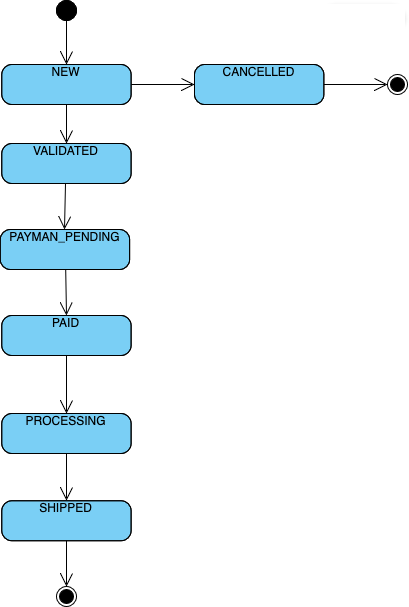
\includegraphics[scale=0.6]{DiagramStanow2.png}
    \caption{Maszyna stanów cyklu życia zamówienia. Źródło: opracowanie własne}
    \label{fig:maszyna-stanow}
\end{figure}

\textbf{Produkt (Product)} reprezentuje pozycję katalogu. Posiada on nazwę, kategorię, opis, cenę z~walutą oraz opcjonalne
zdjęcie. Istotnym elementem modelu jest rozbicie stanu magazynowego produktu na cztery pule ilościowe:
\code{qty} (dostępne), \code{reserved\_qty} (zarezerwowane w~zamówieniach oczekujących na płatność),
\code{paid\_qty} (opłacone). Operacje biznesowe przesuwają ilości pomiędzy tymi pulami. Każde przesunięcie
jest warunkowe i wymaga wystarczjącej ilości w~puli źródłowej. Chroni to przez sprzedażą ponad stan.

\textbf{Płatność (Payment)} wiąże zamówienie z~procesem zapłaty. Posiada dwa stany: \code{PENDING} (utworzona,
oczekuje na realizację) oraz \code{SUCCEEDED} (zakończona). Integracja z rzeczywistym operatorem płatności
pozostaje po za zakresem pracy, więc realizacja płatności jest symulowana. Klient wytwarza żądanie o wytworzenie płatności.
Serwis odpowiada adresem URL płatności i ją finalizuje. Odpowiada to przepływowi stosowanemu przy integracjach
zewnętrznych, co pozwala podmienić symulację na rzeczywistego operatora.

\section{Architektura mikroserwisowa systemu}
\label{sec:architektura-systemu}

Każdemu kontekstowi domenowemu odpowiada osobny mikroserwis: \textbf{order-service} (zamówienia),
\textbf{product-service} (katalog i~stany magazynowe) oraz \textbf{payment-service} (płatności). Interfejs
użytkownika stanowi \textbf{portal obsługi zamówień}. Portal to aplikacja jednostronicowa działająca w~przeglądarce.
Architekturę systemu dopełnia broker komunikatów Apache Kafka, pośredniczący w~asynchronicznej wymianie zdarzeń
pomiędzy usługami. Relacyjna baza danych PostgreSQL. Usługa tożsamości Amazon Cognito. Warstwa brzegowa
(CloudFront i~load balancer), stanowiąca pojedynczy punkt wejścia do systemu. Całość przedstawia
rysunek~\ref{fig:architektura}.

\begin{figure}[H]
    \centering
    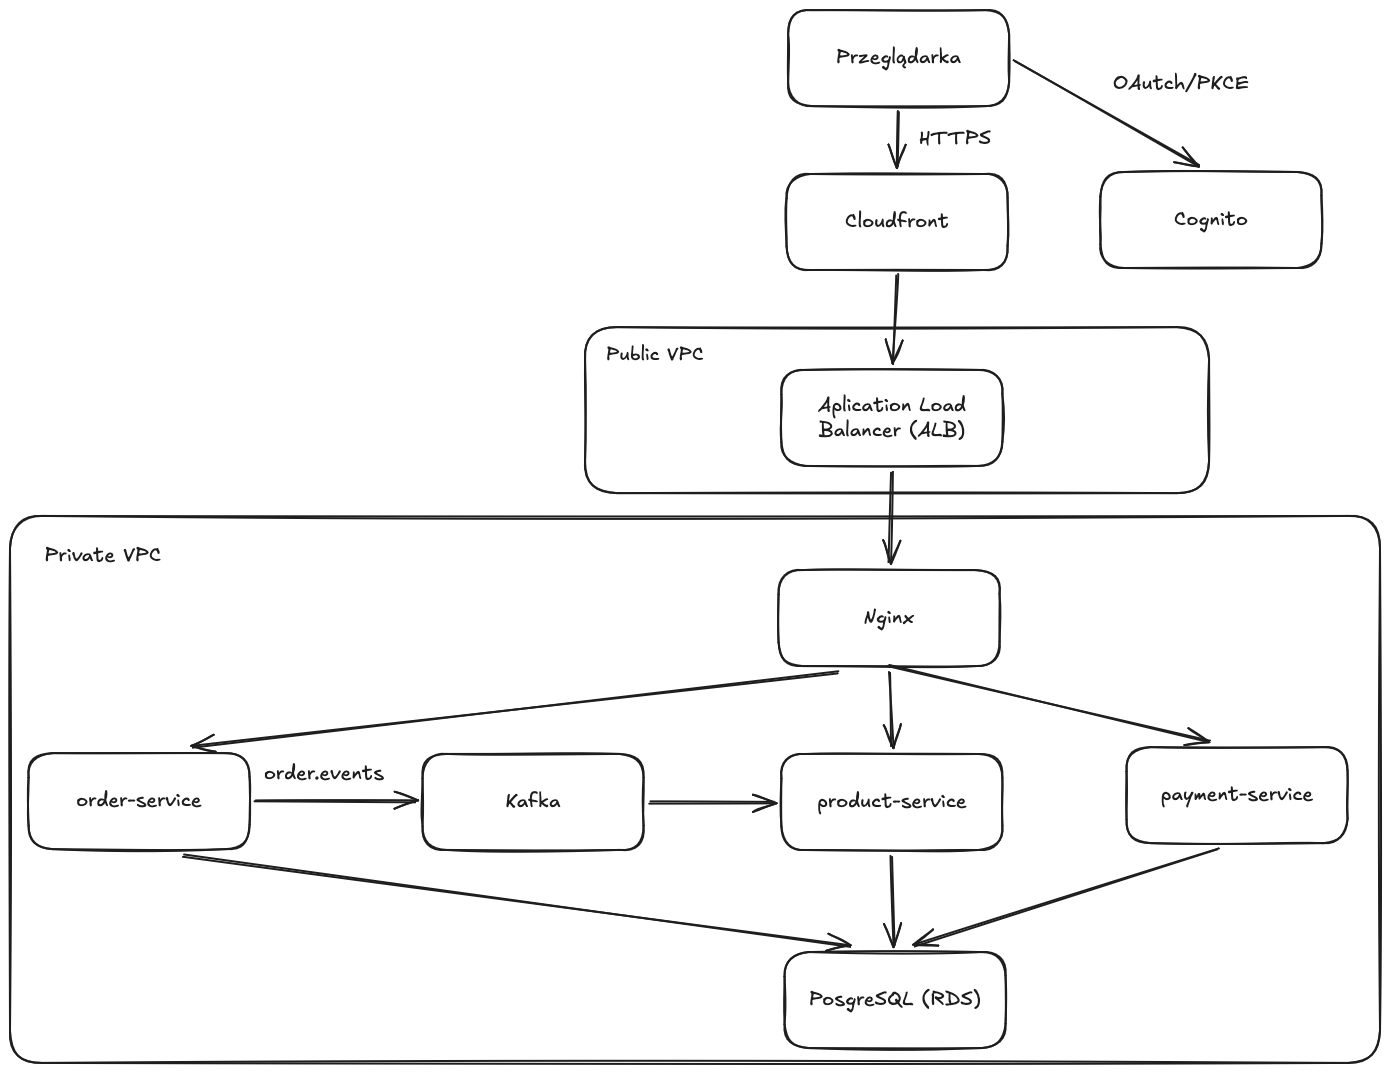
\includegraphics[width=\textwidth]{Architektura_systemu(1).png}
    \caption{Cały ruch użytkownika przechodzi przez~warstwę brzegową (CloudFront\,+\,ALB\,+\,nginx), a~uwierzytelnianie realizuje Amazon Cognito. Komponenty walidacji JWT po~stronie serwisów pominięto dla~czytelności. (źródło: opracowanie własne)}
    \label{fig:architektura}
\end{figure}

Ruch w~systemie przebiega dwiema ścieżkami. Żądania użytkownika są składane przez portal i trafiają poprzez
warstwę brzegową do właściwego serwisu. Dzieje się to za pomocą prefiksu ścieżki i są obsługiwane synchronicznie (sekcja~\ref{sec:projekt-api-i-zdarzen}).
Proces walidacji nie wymaga udziału użytkownika, więc jest obsłużony asynchronicznie poprzez brokera wiadomości.
Podział ten odpowiada zaleceniom przedstawionym w~sekcji~\ref{sec:komunikacja-synchroniczna-asynchroniczna}.

Świadomym odstępstwem od wzorca \emph{database-per-service} jest wykorzystanie wspólnej instancji bazy danych.
Ze względów kosztowych usługi współdzielą jedną instancję PostgreSQL, zachowując jednak rozłączne zestawy tabel,
których wyłącznym właścicielem pozostaje jedna usługa. Wyjątek stanowi proces finalizacji płatności, w~którym
payment-service aktualizuje również tabele zamówień i~produktów. Kompromis ten, jego konsekwencje
oraz docelowe rozwiązanie omówiono w~rozdziałach~\ref{chap:implementacja-mikroserwisow} i~\ref{chap:testy-i-analiza}.

\section{Projekt API REST/JSON oraz kontraktów zdarzeń}
\label{sec:projekt-api-i-zdarzen}

\subsection{Interfejsy REST}
\label{subsec:interfejsy-rest}

Interfejsy usług zaprojektowano zgodnie z~konwencjami REST. Zasoby identyfikowane są ścieżkami, operacje metodami
HTTP, a~reprezentacją danych jest JSON. Zestawienie punktów końcowych przedstawia
tabela~\ref{tab:endpointy-rest}. Wszystkie punkty końcowe, z~wyjątkiem publicznego serwowania zdjęć
produktów, wymagają uwierzytelnienia tokenem JWT (sekcja~\ref{sec:projekt-uwierzytelniania}). Zasoby zamówień
i~płatności zwracane są wyłącznie ich właścicielowi, identyfikowanemu na podstawie tokenu. Listy stronicowane są
parametrami \code{limit} i~\code{offset}, a~katalog produktów filtrowany parametrami zapytania
(\code{category}, \code{minPrice}, \code{maxPrice}, \code{available}).

\begin{table}[H]
    \centering
    \caption{Punkty końcowe REST mikroserwisów}
    \label{tab:endpointy-rest}
    \small
    \begin{tabular}{lp{7.4cm}p{5.2cm}}
        \toprule
        \textbf{Metoda} & \textbf{Ścieżka} & \textbf{Operacja} \\
        \midrule
        \multicolumn{3}{l}{\emph{order-service}} \\
        POST & \code{/api/orders} & złożenie zamówienia (idempotentne) \\
        GET & \code{/api/orders} & lista zamówień klienta \\
        GET & \code{/api/orders/\{id\}} & szczegóły zamówienia \\
        PATCH & \code{/api/orders/\{id\}/status} & zmiana statusu zamówienia \\
        \midrule
        \multicolumn{3}{l}{\emph{product-service}} \\
        GET & \code{/api/products} & lista produktów z~filtrowaniem \\
        GET & \code{/api/products/\{id\}/image/\{imageId\}} & pobranie zdjęcia (publiczne) \\
        \midrule
        \multicolumn{3}{l}{\emph{payment-service}} \\
        POST & \code{/api/v1/payments} & utworzenie żądania płatności \\
        GET & \code{/api/v1/payments} & lista płatności klienta \\
        GET & \code{/api/v1/payments/\{id\}} & szczegóły płatności \\
        POST & \code{/api/v1/payments/\{id\}/pay} & realizacja płatności (symulowana) \\
        \bottomrule
    \end{tabular}
\end{table}

Operacja złożenia zamówienie zaprojektowana została jako idempotentna, według wzorca klucza idempotencji (sekcja~\ref{sec:wzorce-projektowe}).
Klient przekazuje w~nagłówku \code{Idempotency-Key} unikalny identyfikator operacji. Powtórzenie żądania z tym
samym kluczem zwraca pierwotnie utworzone zamówienie zamiast tworzyć duplikat.

\subsection{Kontrakty zdarzeń}
\label{subsec:kontrakty-zdarzen}

Zdarzenia domenowe są przesyłane jako JSON. System order-service publikuje wiadomość na temat \code{order.events}.
Product-service, jako konsument tego zdarzenia, podejmuje próbę atomowej rezerwacji wszystkich pozycji zamówienia.
Zależnie od wyniku ustawia jego status na poprawny albo anulowany. Kwtoy pieniężne są przesyłane jako znaki 
w celu uniknięcia utraty precyzji podczas deserializacji JSON. \ref{lst:order-created}
Pełny przebieg procesu zakupowego przedstawia rysunek~\ref{fig:sekwencja-zamowienia}.

\begin{lstlisting}[caption={Struktura zdarzenia order.created},label={lst:order-created}]
{
  "event": "order.created",
  "orderId": "550e8400-e29b-41d4-a716-446655440000",
  "customerId": "c7f3a2e1-...",
  "status": "NEW",
  "totalAmount": "150.50",
  "currency": "PLN",
  "items": [
    {
      "productId": "9b2d...",
      "productName": "Widget",
      "quantity": 2,
      "unitPrice": "75.25",
      "totalPrice": "150.50"
    }
  ],
  "occurredAt": "2026-06-04T10:30:00Z"
}
\end{lstlisting}

\begin{figure}[H]
    \centering
    \begin{tikzpicture}[
        font=\scriptsize,
        >={Stealth[length=1.6mm]},
        actor/.style={
            rectangle,
            draw,
            thick,
            fill=black!5,
            minimum height=6mm,
            minimum width=18mm,
            align=center,
            font=\scriptsize\bfseries
        },
        msg/.style={->, thick},
        ret/.style={->, densely dashed},
    ]

        \def\portx{0}
        \def\ordx{3.2}
        \def\kafx{6.0}
        \def\prox{8.8}
        \def\payx{11.6}
        \def\toptop{0}
        \def\bot{-8.0}

        \foreach \x/\name in {
            \portx/Portal,
            \ordx/{order-service},
            \kafx/Kafka,
            \prox/{product-service},
            \payx/{payment-service}
        }{
            \node[actor] at (\x,\toptop) {\name};
            \draw[thick, black!40] (\x,-0.4) -- (\x,\bot);
        }

        \draw[msg] (\portx,-1.0) -- node[above]{POST /api/orders} (\ordx,-1.0);
        \draw[ret] (\ordx,-1.6) -- node[above]{201 (NEW)} (\portx,-1.6);

        \draw[msg] (\ordx,-2.3) -- node[above]{order.created} (\kafx,-2.3);
        \draw[msg] (\kafx,-2.9) -- node[above]{order.created} (\prox,-2.9);

        \node[align=center, font=\scriptsize] at (\prox,-3.7)
            {\textit{status $\rightarrow$ VALIDATED}};

        \draw[msg] (\portx,-4.7) -- node[above]{POST /api/v1/payments} (\payx,-4.7);
        \draw[ret] (\payx,-5.3) -- node[above]{201 (PENDING)} (\portx,-5.3);

        \draw[msg] (\portx,-6.1) -- node[above]{POST .../\{id\}/pay} (\payx,-6.1);

        \node[align=center, font=\scriptsize] at (\payx,-6.9)
            {\textit{transakcja:}\\\textit{reserved$\rightarrow$paid,}\\\textit{order PAID}};

        \draw[ret] (\payx,-7.7) -- node[above]{200 (SUCCEEDED)} (\portx,-7.7);

    \end{tikzpicture}
    \caption{Diagram sekwencji przepływu zakupowego. Po~synchronicznym utworzeniu zamówienia jego walidacja przebiega asynchronicznie, według choreografii zdarzeń Kafki (order-service $\rightarrow$ product-service); płatność i~jej finalizacja są~ponownie operacjami synchronicznymi. (źródło: opracowanie własne)}
    \label{fig:sekwencja-zamowienia}
\end{figure}

\section{Wybór technologii implementacyjnych - Go i Vue 3}
\label{sec:wybor-technologii}

Na język implementacji mikroserwisów wybrano \textbf{Go}. Język ten często określany jako język chmury \parencite{medium}.
Ma wiele zalet które idealnie sprawdzają się przy budowaniu mikroserwisów. Go kompiluje się do pojedynczego,
statycznie linkowanego pliku wykonywalnego. Pozwala to budować minimalne obrazy kontenerów pozbawione systemu
operacyjnego (rozdział~\ref{chap:implementacja-mikroserwisow}). Ma bardzo niskie zużycie pamięci i szybki start procesu.
Posiada bardzo lekki model współbieżności (gorutyny). Jest to bardzo ważne przy serwerach obsługujących wiele żądań na raz.
Go poosiada też dojrzały ekosystem bibliotek. Spośród nich wykorzystano m.in. router HTTP \code{chi}, sterownik PostgreSQL 
\code{pgx}, klienta Kafki \code{franz-go} oraz bibliotekę \code{jwx} do weryfikacji tokenów JWT.
Jedną z wielkich zalet Go jest też bardzo bogata biblioteka standardowa, która pozwala na nie używanie ciężkich
frameworków.

Warstwę frontendu zrealizowano we frameworku \textbf{Vue~3} z~językiem \textbf{TypeScript}. Vue~3 oferuje
reaktywny model danych i~kompozycyjne API sprzyjające wielokrotnemu użyciu logiki. Statycznie typowany
TypeScript pozwala wykryć znaczną ilość błędów w etapie kompilacji. Stan aplikacji (sesja użytkownika, koszyk)
zarządzany jest biblioteką Pinia, a~proces budowania narzędziem Vite. Szczegóły architektury portalu przedstawiono
w~rozdziale~\ref{chap:implementacja-portalu}.

\section{Projekt bazy danych i persystencji - PostgreSQL}
\label{sec:projekt-bazy-danych}

Warstwę persystencji oparto na relacyjnej bazie danych \textbf{PostgreSQL}. PostgreSQL jest obecnie jedną z najlepiej
rozwijanych baz danych. Bardzo dobra transakcyjność ACID była niezbędna przy warunkowych przesunięciach 
stanów magazynowych i~finalizacji płatności. Dostępność PostgreSQL jako w~pełni zarządzanej usługi Amazon RDS
była kolejnym powodem wybrania tego silnika (sekcja~\ref{subsec:rds}).

Schemat głównej tabeli zamówień przedstawiono na~fragmencie~\ref{lst:schemat-orders}. Identyfikatory zapisano jako
\code{TEXT}. Pozycje zamówienia i~adres dostawy w~kolumnach \code{JSONB}. Pełną historię przejść między stanami
utrwala kolumna \code{history}.

\begin{lstlisting}[caption={Fragment kodu SQL definiujący tabelę orders},label={lst:schemat-orders},language=SQL]
CREATE TABLE orders (
    id               TEXT          PRIMARY KEY,
    customer_id      TEXT          NOT NULL,
    status           TEXT          NOT NULL,
    items            JSONB         NOT NULL,
    total_amount     NUMERIC(20,4) NOT NULL,
    currency         CHAR(3)       NOT NULL,
    delivery_address JSONB         NOT NULL,
    history          JSONB         NOT NULL,
    created_at       TIMESTAMPTZ   NOT NULL,
    updated_at       TIMESTAMPTZ   NOT NULL
);
\end{lstlisting}

Tabelę uzupełniają indeksy na kolumnach \code{customer\_id} i~\code{created\_at}, wspierające najczęstsze zapytania
systemu. Tabela \code{idempotency\_keys} (listing~\ref{lst:schemat-idempotency_keys}) wiąże klucze idempotencji
z~identyfikatorami utworzonych zamówień, dzięki czemu powtórzone żądanie z~tym samym kluczem nie~tworzy duplikatu.

\begin{lstlisting}[caption={Schemat tabeli idempotency keys},label={lst:schemat-idempotency_keys},language=SQL]
CREATE TABLE idempotency_keys (
    key        TEXT PRIMARY KEY,
    order_id   TEXT        NOT NULL,
    created_at TIMESTAMPTZ NOT NULL DEFAULT NOW()
);
\end{lstlisting}

Serwis produktów przechowuje katalog w~tabeli \code{products} (listing~\ref{lst:schemat-products}). Stan magazynowy zamodelowano czterema
kolumnami ilościowymi (\code{qty}, \code{reserved\_qty}, \code{paid\_qty}, \code{shipped\_qty}) z~ograniczeniami
\code{CHECK} wykluczającymi wartości ujemne. Dzięki czemu niezmiennik nieujemności stanów magazynowych
egzekwowany jest również na poziomie bazy.

\begin{lstlisting}[caption={Schemat tabeli products},label={lst:schemat-products},language=SQL]
CREATE TABLE products (
    id           TEXT PRIMARY KEY,
    name         TEXT          NOT NULL,
    category     TEXT          NOT NULL,
    description  TEXT          NOT NULL,
    price        NUMERIC(20,4) NOT NULL,
    currency     CHAR(3)       NOT NULL,
    qty          INTEGER       NOT NULL CHECK (qty >= 0),
    reserved_qty INTEGER       NOT NULL DEFAULT 0 CHECK (reserved_qty >= 0),
    paid_qty     INTEGER       NOT NULL DEFAULT 0 CHECK (paid_qty >= 0),
    shipped_qty  INTEGER       NOT NULL DEFAULT 0 CHECK (shipped_qty >= 0),
    created_at   TIMESTAMPTZ   NOT NULL,
    updated_at   TIMESTAMPTZ   NOT NULL
);
\end{lstlisting}

Zdjęcia produktów przechowywane są w~tabeli \code{product\_images} w~kolumnie binarnej \code{BYTEA},
wraz z~typem MIME i~rozmiarem; jej schemat przedstawia listing~\ref{lst:schemat-images}.

\begin{lstlisting}[caption={Schemat tabeli images},label={lst:schemat-images},language=SQL]
CREATE TABLE IF NOT EXISTS product_images (
    product_id   TEXT PRIMARY KEY REFERENCES products (id) ON DELETE CASCADE,
    id           TEXT        NOT NULL,
    content_type TEXT        NOT NULL,
    file_name    TEXT,
    byte_size    BIGINT      NOT NULL CHECK (byte_size >= 0),
    data         BYTEA       NOT NULL,
    created_at   TIMESTAMPTZ NOT NULL DEFAULT NOW()
);
\end{lstlisting}

Serwis płatności utrzymuje tabelę \code{payments}, wiążącą płatność
z~zamówieniem i~klientem oraz rejestrującą znacznik czasu finalizacji; jej schemat przedstawia
listing~\ref{lst:schemat-payments}.

\begin{lstlisting}[caption={Schemat tabeli payments},label={lst:schemat-payments},language=SQL]
CREATE TABLE IF NOT EXISTS payments (
    id           TEXT PRIMARY KEY,
    order_id     TEXT        NOT NULL REFERENCES orders (id),
    customer_id  TEXT        NOT NULL,
    status       TEXT        NOT NULL,
    created_at   TIMESTAMPTZ NOT NULL,
    updated_at   TIMESTAMPTZ NOT NULL,
    completed_at TIMESTAMPTZ
);
\end{lstlisting}

\section{Asynchroniczna wymiana zdarzeń - Apache Kafka}
\label{sec:kafka}

Rolę brokera komunikatów pełni \textbf{Apache Kafka} . Jest to rozproszony dziennik zdarzeń (\emph{distributed log}),
w~którym komunikaty zapisywane są trwale, w~kolejności, do nazwanych tematów (\emph{topics}) dzielonych na
partycje \parencite{kleppmann2017}. Model konsumpcji oparty jest na grupach konsumentów. Każda grupa utrzymuje własne
przesunięcie (\emph{offset}) w~temacie, dzięki czemu wielu niezależnych odbiorców może przetwarzać ten sam strumień
zdarzeń, a~konsument po awarii wznawia przetwarzanie od ostatniej zatwierdzonej pozycji. Ta właściwość odróżnia Kafkę 
od klasycznych kolejek komunikatów i~czyni ją naturalnym nośnikiem zdarzeń domenowych.

W~systemie zdefiniowano dwa tematy. \code{order.events}, do którego order-service publikuje zdarzenia cyklu życia
zamówień. \code{product.events}, do którego product-service publikuje wyniki walidacji. Product-service
konsumuje temat \code{order.events} w~ramach grupy \code{product-service}. Kafka gwarantuje dostarczenie
\emph{co najmniej raz}, zatem konsumenci zaprojektowani są idempotentnie.Powtórne przetworzenie zdarzenia
\code{order.created} nie podwaja rezerwacji, ponieważ operacja rezerwacji dla danego zamówienia jest skuteczna
tylko przy pierwszym wykonaniu. Broker uruchamiany jest w~klastrze Kubernetes w~trybie KRaft (bez komponentu
ZooKeeper), w~konfiguracji jednowęzłowej. Wystarcza to dla środowiska demonstracyjnego, której ograniczenia
omówiono w~rozdziale~\ref{chap:testy-i-analiza}.

\section{Projekt uwierzytelniania i autoryzacji}
\label{sec:projekt-uwierzytelniania}

Uwierzytelnianie użytkowników oparto na protokole \textbf{OAuth~2.0} \parencite{rfc6749} z~warstwą tożsamości OpenID
Connect, z~Amazon Cognito w~roli serwera autoryzacji (sekcja~\ref{subsec:cognito}). Ponieważ klientem jest
aplikacja jednostronicowa, zastosowano przepływ \emph{authorization code} z~rozszerzeniem \textbf{PKCE} (\emph{Proof Key for Code Exchange})
\parencite{rfc7636}. Portal generuje przy każdym logowaniu jednorazowy weryfikator, którego skrót dołącza do żądania
autoryzacji, a~oryginał przedstawia przy wymianie kodu na tokeny. Uniemożliwia to wykorzystanie przechwyconego
kodu autoryzacyjnego przez stronę trzecią.

Przebieg logowania jest następujący. Portal przekierowuje użytkownika do hostowanego interfejsu logowania Cognito.
Po poprawnym uwierzytelnieniu Cognito zwraca kod autoryzacyjny na zarejestrowany adres zwrotny portalu, który
wymienia go wraz z~weryfikatorem PKCE na tokeny JWT. Hasła użytkowników nigdy nie przepływają przez
aplikację. Uzyskany token dołączany jest do każdego żądania API w~nagłówku \code{Authorization}.

\begin{figure}[H]
    \centering
    \begin{tikzpicture}[
        font=\scriptsize,
        >={Stealth[length=1.6mm]},
        actor/.style={rectangle, draw, thick, fill=black!5, minimum height=6mm,
                      minimum width=20mm, align=center, font=\scriptsize\bfseries},
        msg/.style={->, thick},
        ret/.style={->, densely dashed},
    ]
        \def\usrx{0} \def\spax{3.6} \def\cogx{7.6} \def\svcx{11.0}
        \def\bot{-8.0}
        \foreach \x/\name in {\usrx/Użytkownik, \spax/{Portal (SPA)},
                              \cogx/{Cognito}, \svcx/{Mikroserwis}} {
            \node[actor] at (\x,0) {\name};
            \draw[thick, black!40] (\x,-0.4) -- (\x,\bot);
        }
        \draw[msg] (\usrx,-1.0) -- node[above]{,,Zaloguj''} (\spax,-1.0);
        \node[align=center, font=\scriptsize] at (\spax,-1.7)
            {\textit{generuj verifier}\\\textit{+ challenge (S256)}};
        \draw[msg] (\spax,-2.5) -- node[above, align=center]{redirect:\\code\_challenge} (\cogx,-2.5);
        \draw[msg] (\cogx,-3.2) -- node[above]{formularz logowania} (\usrx,-3.2);
        \draw[msg] (\usrx,-3.9) -- node[above]{login + hasło} (\cogx,-3.9);
        \draw[ret] (\cogx,-4.6) -- node[above, align=center]{redirect:\\code} (\spax,-4.6);
        \draw[msg] (\spax,-5.3) -- node[above, align=center]{code + verifier\\$\rightarrow$ /oauth2/token} (\cogx,-5.3);
        \draw[ret] (\cogx,-6.0) -- node[above]{tokeny JWT} (\spax,-6.0);
        \draw[msg] (\spax,-6.9) -- node[above, align=center]{żądanie API\\+ Bearer JWT} (\svcx,-6.9);
        \node[align=center, font=\scriptsize] at (\svcx,-7.6)
            {\textit{weryfikacja}\\\textit{podpisu (JWKS)}};
    \end{tikzpicture}
    \caption{Przepływ uwierzytelniania OAuth~2.0 \emph{authorization code} z~rozszerzeniem PKCE. Portal generuje weryfikator i~jego skrót; po~zalogowaniu wymienia kod autoryzacyjny na~tokeny JWT. Każdy mikroserwis weryfikuje podpis tokenu samodzielnie, na~podstawie kluczy publicznych Cognito (JWKS). (źródło: opracowanie własne)}
    \label{fig:pkce}
\end{figure}

Autoryzację zaprojektowano w~modelu zdecentralizowanym. Każdy mikroserwis samodzielnie weryfikuje podpis
i~zawartość tokenu na podstawie publicznych kluczy Cognito (zbioru JWKS), bez odwołań do centralnej usługi sesji.
Dzięki czemu uwierzytelnienie żądania nie wprowadza dodatkowej zależności sieciowej ani pojedynczego punktu
awarii. Tożsamość klienta odczytywana z~tokenu wyznacza zakres dostępu do danych (klient widzi wyłącznie własne
zamówienia i~płatności). Szczegóły weryfikacji tokenów po stronie usług przedstawiono w~rozdziale~\ref{chap:implementacja-mikroserwisow}, 
a~implementację przepływu PKCE w~portalu w~rozdziale~\ref{chap:implementacja-portalu}.
\chapter{Implementacja mikroserwisów}
\label{chap:implementacja-mikroserwisow}

Rozdział ten przedstawia implementację trzech mikroserwisów systemu w~języku Go. Omówiono wspólną strukturę
i~wzorce dzielone przez wszystkie usługi, a~następnie logikę biznesową każdej z~nich, warstwę zdarzeń, mechanizm
uwierzytelniania, obserwowalność, konteneryzację oraz testy. Prezentowane listingi pochodzą bezpośrednio z~kodu
źródłowego systemu.

\section{Struktura projektu i wspólne wzorce serwisów}
\label{sec:struktura-projektu}

Wszystkie trzy serwisy zbudowano według tego samego szablonu, opartego na architekturze heksagonalnej
(\emph{ports and adapters}). Logika domenowa stanowi rdzeń niezależny od technologii. Komunikacja ze światem
zewnętrznym przebiega przez HTTP. Baza danych, broker komunikatów odbywa się poprzez wymienne adaptery, sprzęgnięte
z~rdzeniem wyłącznie interfejsami. Strukturę katalogów serwisu zamówień przedstawia listing~\ref{lst:struktura-serwisu}.

\begin{lstlisting}[caption={Struktura katalogów serwisu zamówień},label={lst:struktura-serwisu}]
order-service/
|-- main.go               # punkt wejścia, złożenie zależności
|-- Dockerfile
`-- internal/
    |-- auth/             # weryfikacja JWT (Cognito)
    |-- config/           # konfiguracja ze zmiennych środowiskowych
    |-- db/               # pula połączeń PostgreSQL, migracje
    |-- metrics/          # definicje metryk Prometheus
    |-- producer/         # producent zdarzeń Kafka
    |-- server/           # serwery HTTP: API i techniczny
    `-- order/            # kontekst domenowy
        |-- domain/       # encje, maszyna stanów, niezmienniki
        |-- service/      # przypadki użycia (logika aplikacyjna)
        |-- repository/   # adapter PostgreSQL
        |-- events/       # definicje zdarzeń domenowych
        `-- api/          # handlery HTTP, DTO, walidacja wejścia
\end{lstlisting}

Zależności składane są jawnie w~funkcji \code{main}, bez wstrzykiwania zależności. Granice pomiędzy
warstwami wyznaczają małe interfejsy definiowane po stronie konsumenta, co jest idiomatycznym wzorcem języka Go.
Tworzy to pakiety bez zewnętrznych zależności co pozwala testować logikę biznesową w odpowiedniej izolacji.

Każdy serwis uruchamia dwa niezależne serwery HTTP na oddzielnych portach. Serwer \textbf{API} obsługuje ruch biznesowy. Serwer
\textbf{techniczny} udostępnia punkty końcowe eksploatacyjne: \code{/ping} (kontrola zdrowia), 
\code{/metrics} (metryki Prometheus), \code{/version} oraz \code{/debug/pprof} (profilowanie procesu).
Rozdzielenie portów gwarantuje, że dane eksploatacyjne nigdy nie są osiągalne ścieżką publiczną, nawet przy błędnej konfiguracji routingu.

Konfiguracja serwisów realizuje wzorzec konfiguracji zewnętrznej (sekcja~\ref{sec:wzorce-projektowe}). Wszystkie
parametry wczytywane są ze zmiennych środowiskowych do struktur Go.

\section{Serwis zamówień - logika biznesowa, maszyna stanów i idempotencja}
\label{sec:order-service}

Serwis zamówień realizuje utworzenie zamówienia oraz pobranie i~listowanie zamówień klienta.
Tworząc zamówienie, warstwa domenowa egzekwuje niezmienniki: niepustą listę pozycji,
dodatnie ilości, poprawny kod waluty oraz zgodność kwoty całkowitej z~sumą pozycji.

Centralnym elementem domeny jest maszyna stanów zamówienia. Dozwolone przejścia zakodowano jako strukturę danych.
Mapę stanów osiągalnych z~każdego stanu, dzięki czemu cykl życia zamówienia opisany jest w~jednym miejscu kodu 
i~bezpośrednio odpowiada diagramowi z~projektu (sekcja~\ref{sec:model-domenowy}). Implementację przedstawia 
listing~\ref{lst:maszyna-stanow}. Stany terminalne nie posiadają wpisu w~mapie, więc żadne przejście z~nich nie jest możliwe.

\begin{lstlisting}[caption={Implementacja maszyny stanów zamówienia},label={lst:maszyna-stanow},language=Go]
// allowedTransitions defines the order lifecycle.
//
//  NEW -> VALIDATED -> PAYMENT_PENDING -> PAID -> PROCESSING -> SHIPPED
//  plus CANCELLED / FAILED reachable from any non-terminal state.
var allowedTransitions = map[OrderStatus]map[OrderStatus]struct{}{
    OrderStatusNew:            {OrderStatusValidated: {}, OrderStatusCancelled: {}, OrderStatusFailed: {}},
    OrderStatusValidated:      {OrderStatusPaymentPending: {}, OrderStatusCancelled: {}, OrderStatusFailed: {}},
    OrderStatusPaymentPending: {OrderStatusPaid: {}, OrderStatusCancelled: {}, OrderStatusFailed: {}},
    OrderStatusPaid:           {OrderStatusProcessing: {}, OrderStatusCancelled: {}, OrderStatusFailed: {}},
    OrderStatusProcessing:     {OrderStatusShipped: {}, OrderStatusCancelled: {}, OrderStatusFailed: {}},
}

func CanTransition(from, to OrderStatus) bool {
    if from == to {
        return false
    }
    next, ok := allowedTransitions[from]
    if !ok {
        return false
    }
    _, ok = next[to]
    return ok
}
\end{lstlisting}

Każde wykonane przejście dopisywane jest do historii zamówienia (stan poprzedni, nowy, znacznik czasu, opcjonalny
powód), utrwalanej w~kolumnie \code{JSONB}. Daje to pełny ślad cyklu życia każdego zamówienia.

Idempotencję operacji utworzenia zamówienia zrealizowano na poziomie bazy danych, w~sposób odporny na wyścigi
współbieżnych żądań (listing~\ref{lst:idempotencja}). Klucz z~nagłówka \code{Idempotency-Key} zapisywany jest
instrukcją \code{INSERT} z~klauzulą \code{ON CONFLICT}. Jeśli klucz został już zajęty, zapytanie zamiast
zakończyć się błędem zwraca identyfikator zamówienia utworzonego pierwotnie, a~serwis odpowiada klientowi tym
właśnie zamówieniem. Rozstrzygnięcie kolizji następuje zatem atomowo w~jednym zapytaniu, bez okna czasowego
pomiędzy sprawdzeniem a~zapisem klucza.

\begin{lstlisting}[caption={Atomowe zajęcie klucza idempotencji},label={lst:idempotencja},language=Go]
func (r *Postgres) SaveIdempotencyKey(ctx context.Context, key, orderID string) (string, error) {
    var stored string
    err := r.pool.QueryRow(ctx, `
        INSERT INTO idempotency_keys (key, order_id) VALUES ($1, $2)
        ON CONFLICT (key) DO UPDATE SET key = idempotency_keys.key
        RETURNING order_id
    `, key, orderID).Scan(&stored)
    if err != nil {
        return "", fmt.Errorf("save idempotency key: %w", err)
    }
    if stored != orderID {
        return stored, domain.ErrIdempotencyExists
    }
    return "", nil
}
\end{lstlisting}

Po utrwaleniu zamówienia serwis publikuje zdarzenie \code{order.created}.

\section{Serwis produktów - katalog i rezerwacja stanów magazynowych}
\label{sec:product-service}

Serwis produktów pełni dwie role. Synchronicznie obsługuje katalog (listowanie z~filtrowaniem po kategorii,
przedziale cenowym i~dostępności, obsługę zdjęć przechowywanych w~kolumnie \code{BYTEA}).
Oraz asynchronicznie uczestniczy w~walidacji zamówień jako konsument zdarzeń.

Rezerwacja stanów magazynowych realizowana jest operacją wsadową obejmującą wszystkie pozycje zamówienia w~jednej
transakcji bazodanowej. Rezerwacja jest więc niepodzielna. Nie istnieje stan, w~którym część pozycji zamówienia
została zarezerwowana, a~część nie. Samo przesunięcie ilości pomiędzy pulami wykonywane jest warunkową instrukcją
\code{UPDATE}. Warunek (\code{qty >= \$2}) gwarantuje poprawność również przy współbieżnej rezerwacji tego
samego produktu przez dwa zamówienia. Przegrywające zapytanie nie zmodyfikuje żadnego wiersza, co serwis
interpretuje jako niewystarczający stan magazynowy.

Po otrzymaniu zdarzenia \code{order.created} konsument dekoduje je, waliduje i~podejmuje próbę rezerwacji.
W~zależności od wyniku publikuje \code{order.validated} albo \code{order.reservation\_failed}.

Rozwiązaniem przejściowym, jest sposób domknięcia pętli walidacji. Docelowo order-service powinien 
konsumować temat \code{product.events} i~sam zmieniać status zamówienia. W~bieżącej
wersji systemu konsument ten nie istnieje. Product-service aktualizuje więc status zamówienia
(\code{VALIDATED} lub \code{CANCELLED}) bezpośrednio w~tabeli zamówień, równolegle z~publikacją zdarzenia.
Kompromis ten narusza zasadę wyłącznej własności danych (sekcja~\ref{sec:charakterystyka-mikroserwisow})
i~został świadomie przyjęty jako etap pośredni. Jego usunięcie wskazano jako kierunek rozwoju
w~podsumowaniu pracy.

\section{Serwis płatności - transakcyjna obsługa procesu płatności}
\label{sec:payment-service}

Serwis płatności obsługuje utworzenie żądania płatności dla zamówienia (zwracając klientowi adres URL płatności)
oraz jej finalizację. Finalizacja jest najbardziej krytyczną operacją systemu. Musi jednocześnie i~niepodzielnie
przenieść zarezerwowane ilości wszystkich pozycji zamówienia do puli opłaconych, oznaczyć zamówienie jako
\code{PAID} oraz płatność jako \code{SUCCEEDED}. Zrealizowano ją jako pojedynczą transakcję bazodanową
z~blokadami wierszy.

Transakcja rozpoczyna się pobraniem płatności i~zamówienia z~klauzulą \code{FOR UPDATE}, co wyklucza równoległą
finalizację tej samej płatności. Następnie weryfikowane są warunki: przynależność płatności i~zamówienia do
uwierzytelnionego klienta, poprawność pozycji oraz to, czy zamówienie znajduje się w~stanie dopuszczającym
zapłatę. Przy czym ponowna finalizacja płatności już zakończonej nie jest błędem, lecz zwraca jej bieżący stan
(operacja jest idempotentna). Dla każdej pozycji zamówienia wykonywane jest warunkowe przesunięcie ilości
(listing~\ref{lst:platnosc-update}). Niepowodzenie któregokolwiek przesunięcia wycofuje całą transakcję.

\begin{lstlisting}[caption={Warunkowe przesunięcie ilości w transakcji płatności},label={lst:platnosc-update},language=Go]
tag, err := tx.Exec(ctx, `
    UPDATE products
    SET reserved_qty = reserved_qty - $2,
        paid_qty = paid_qty + $2
    WHERE id = $1 AND reserved_qty >= $2
`, item.ProductID, item.Quantity)
\end{lstlisting}

Transakcja ta obejmuje tabele trzech kontekstów domenowych (płatności, zamówień i~produktów), co stanowi opisany
w~sekcji~\ref{sec:architektura-systemu} świadomy kompromis względem wzorca \emph{database-per-service}.
Współdzielenie jednej instancji baz gwarantujący silną spójność najbardziej wrażliwej operacji
systemu bez implementacji rozproszonej sagi.

\section{Publikacja i konsumpcja zdarzeń Kafka}
\label{sec:implementacja-kafka}

Warstwę zdarzeń zrealizowano biblioteką \code{franz-go}. Producent serializuje zdarzenia do JSON i~publikuje je
do skonfigurowanego tematu w~trybie nieblokującym. Publikacja nie wydłuża obsługi żądania HTTP, ponieważ rekordy
trafiają do wewnętrznego bufora klienta i~są wysyłane wsadowo w~tle. Listing~\ref{lst:kafka-producer} przedstawia
konfigurację producenta w~order-service oraz metodę publikującą zdarzenie. Krótki czas zwłoki
(\code{ProducerLinger}) pozwala grupować rekordy w~większe wsady, ograniczenie bufora
(\code{MaxBufferedRecords}) chroni proces przed nieograniczonym wzrostem pamięci przy niedostępności brokera,
a~partycjonowanie po kluczu zachowuje kolejność zdarzeń dotyczących tego samego zamówienia.

\begin{lstlisting}[caption={Konfiguracja i nieblokująca publikacja zdarzeń w order-service},label={lst:kafka-producer},language=Go]
func kafkaOptionsNotifier(topic, urls string) []kgo.Opt {
    return []kgo.Opt{
        kgo.SeedBrokers(strings.Split(urls, ",")...),
        kgo.DefaultProduceTopic(topic),
        kgo.ProducerLinger(time.Duration(50) * time.Millisecond),
        kgo.MaxBufferedRecords(20_000),
        kgo.RecordPartitioner(kgo.StickyKeyPartitioner(nil)),
    }
}

func (n *EventNotifier) Notify(log any) error {
    if !n.enabled {
        return nil
    }
    b, err := json.Marshal(log)
    if err != nil {
        return fmt.Errorf("unable to marshal log: %w", err)
    }
    n.producer.Produce(context.Background(), kgo.SliceRecord(b), nil)

    return nil
}
\end{lstlisting}

Konsument w~product-service działa w~ramach grupy konsumentów \code{product-service}, dzięki czemu pozycja odczytu
tematu \code{order.events} jest trwała. Po restarcie serwis wznawia przetwarzanie od ostatniego zatwierdzonego
przesunięcia, nie gubiąc zdarzeń opublikowanych w~czasie jego niedostępności. Pętla odczytu
(listing~\ref{lst:kafka-consumer}) pobiera wsady rekordów i~przekazuje każdy z~nich do funkcji obsługi
przekazanej przy konstrukcji konsumenta. Błąd obsługi pojedynczego rekordu jest logowany, lecz nie zatrzymuje
przetwarzania kolejnych zdarzeń.

\begin{lstlisting}[caption={Pętla konsumenta zdarzeń w product-service},label={lst:kafka-consumer},language=Go]
opts := []kgo.Opt{
    kgo.SeedBrokers(strings.Split(cfg.URL, ",")...),
    kgo.ConsumerGroup(cfg.Group),
    kgo.ConsumeTopics(cfg.Topic),
}

func (c *Consumer) Run(ctx context.Context) error {
    ...
    defer c.client.Close()

    slog.Info("kafka consumer started")
    for {
        if ctx.Err() != nil {
            return nil
        }

        fetches := c.client.PollFetches(ctx)
        if fetches.IsClientClosed() {
            return nil
        }
        fetches.EachError(func(topic string, partition int32, err error) {
            if errors.Is(err, context.Canceled) {
                return
            }
            slog.Error("kafka fetch error", "topic", topic,
                "partition", partition, "err", err)
        })

        fetches.EachRecord(func(r *kgo.Record) {
            if err := c.handle(ctx, r.Value); err != nil {
                slog.Error("handle kafka record failed", "topic", r.Topic,
                    "offset", r.Offset, "err", err)
            }
        })
    }
}
\end{lstlisting}

\section{Walidacja tokenów JWT i integracja z Cognito}
\label{sec:implementacja-auth}

Uwierzytelnianie żądań zrealizowano jako middleware HTTP, włączany przed handlery wszystkich chronionych punktów
końcowych. Middleware wydobywa token z~nagłówka \code{Authorization}, przekazuje go do weryfikatora, a~po pomyślnej
weryfikacji umieszcza tożsamość klienta w~kontekście żądania. Skąd odczytują ją handlery, zawężając operacje 
do zasobów uwierzytelnionego użytkownika.

Produkcyjny weryfikator (listing~\ref{lst:cognito-verify}) opiera się na bibliotece \code{jwx}. Klucze publiczne
puli użytkowników pobierane są ze~standardowego adresu JWKS i~buforowane lokalnie z~okresowym odświeżaniem
(od~15~minut do~24~godzin).

\begin{lstlisting}[caption={Weryfikacja tokenu JWT wobec kluczy Cognito},label={lst:cognito-verify},language=Go]
func (v *CognitoVerifier) Verify(_ context.Context, raw string) (jwt.Token, error) {
    tok, err := jwt.Parse(
        []byte(raw),
        jwt.WithKeySet(v.keySet),
        jwt.WithValidate(true),
        jwt.WithIssuer(v.issuer),
        jwt.WithAcceptableSkew(30*time.Second),
    )
    if err != nil {
        return nil, fmt.Errorf("token verify: %w", err)
    }

    var tokenUse string
    if err := tok.Get("token_use", &tokenUse); err != nil {
        return nil, fmt.Errorf("token_use claim missing: %w", err)
    }
    if _, ok := v.allowedTokenUse[tokenUse]; !ok {
        return nil, fmt.Errorf("token_use %q not allowed", tokenUse)
    }
    ...
}
\end{lstlisting}

Na potrzeby pracy lokalnej przewidziano tryb deweloperski (\code{COGNITO\_ENABLED=false}), w~którym tożsamość
klienta przekazywana jest jawnie w~nagłówku żądania. Tryb ten nie jest dostępny w~konfiguracji produkcyjnej.

\section{Obserwowalność serwisów}
\label{sec:obserwowalnosc-serwisow}

Każdy serwis publikuje metryki Prometheus w~przestrzeni nazw odpowiadającej usłudze (prefiksy \code{order\_},
\code{product\_}, \code{payment\_}). Warstwa HTTP instrumentowana jest middleware'em zliczającym żądania, mierzącym histogram czasów
obsługi oraz liczbę żądań w~toku. Obok metryk technicznych serwisy publikują metryki domenowe, które pozwalają obserwować system
w~kategoriach biznesowych, a~nie wyłącznie infrastrukturalnych.

Logowanie zrealizowano pakietem standardowym \code{slog} z~formatem JSON i~konfigurowalnym poziomem. Serwer
techniczny każdej usługi udostępnia ponadto kontrolę zdrowia \code{/ping}, informację o~wersji \code{/version}
oraz profilowanie \code{pprof}, pozwalające diagnozować zużycie procesora i~pamięci działającego procesu.

\section{Konteneryzacja serwisów}
\label{sec:konteneryzacja-serwisow}

Obrazy kontenerów budowane są wieloetapowo (listing~\ref{lst:dockerfile}). Etap budowania, oparty na obrazie
\code{golang:alpine}, kompiluje statycznie linkowany plik wykonywalny. Osobne kopiowanie plików
\code{go.mod} i~\code{go.sum} oraz montowane pamięci podręczne modułów i~kompilatora pozwalają przy niezmienionych
zależnościach pominąć ich ponowne pobieranie. Obraz docelowy to \code{distroless/static}. Czyli obraz pozbawiony
powłoki, menedżera pakietów i~jakichkolwiek narzędzi systemowych. Zawierający wyłącznie skompilowany plik binarny
i~certyfikaty TLS. Uruchamiany jest jako użytkownik nieuprzywilejowany (\code{nonroot}). Minimalizuje to zarówno
rozmiar obrazu, jak i~powierzchnię ataku.

\begin{lstlisting}[caption={Wieloetapowy Dockerfile serwisu zamówień},label={lst:dockerfile},language=bash]
FROM golang:1.26.3-alpine AS build
WORKDIR /src

COPY go.mod go.sum ./
RUN --mount=type=cache,target=/go/pkg/mod \
    go mod download

COPY . .
RUN --mount=type=cache,target=/go/pkg/mod \
    --mount=type=cache,target=/root/.cache/go-build \
    CGO_ENABLED=0 GOOS=linux go build \
    -trimpath -ldflags="-s -w" \
    -o /out/order-service .

FROM gcr.io/distroless/static-debian12:nonroot
COPY --from=build /out/order-service /order-service
EXPOSE 9002 9090
USER nonroot
ENTRYPOINT ["/order-service"]
\end{lstlisting}

\section{Testy jednostkowe i integracyjne}
\label{sec:testy-backend}

Testy serwisów napisano w~standardowym frameworku testowym Go. W~konwencji testów tabelarycznych. Pokrywają one
dwa poziomy. Poziom domenowy weryfikuje logikę biznesową w~pełnej izolacji.

Testy uruchamiane są z~włączonym detektorem wyścigów (\code{go test -race}) oraz losową kolejnością wykonywania
(\code{-shuffle=on}). Pozwala to wykrywać odpowiednio błędy współbieżności i~ukryte zależności pomiędzy testami.
Te same polecenia wykonywane są automatycznie przy każdej zmianie kodu w~potoku ciągłej integracji. 
Testy obciążeniowe systemu wdrożonego w~środowisku docelowym omówiono odrębnie w~rozdziale~\ref{chap:testy-i-analiza}.
\chapter{Implementacja portalu obsługi zamówień}
\label{chap:implementacja-portalu}

Interfejs użytkownika systemu stanowi portal obsługi zamówień. Aplikacja jednostronicowa (SPA) działająca
w~przeglądarce, realizująca pełny przepływ zakupowy. Od przeglądania katalogu, przez koszyk i~złożenie zamówienia,
po płatność i~wgląd w~historię zamówień. Rozdział omawia architekturę aplikacji, jej widoki, warstwę komunikacji
z~interfejsami REST mikroserwisów, implementację logowania w~przepływie OAuth~2.0 z~PKCE oraz testy.

\section{Architektura aplikacji frontendowej}
\label{sec:architektura-frontendu}

Aplikację zbudowano we frameworku Vue~3 z~językiem TypeScript w~trybie ścisłym (\code{strict}), z~użyciem
kompozycyjnego API. Kod podzielony jest na warstwy o~jasno określonych odpowiedzialnościach. Katalog
\code{views} zawiera widoki powiązane z~trasami routera. Katalog \code{components} zawiera współdzielone komponenty powłoki
aplikacji. Ścieżka \code{stores} zawiera magazyny stanu Pinia, a \code{services} warstwę dostępu do API.
Na koniec \code{composables} ma funkcje kompozycyjne wielokrotnego użytku. Warstwę
prezentacji ostylowano biblioteką Tailwind CSS z~paletą i~typografią wzorowaną na Material Design~3.
Nawigację obsługuje Vue Router z~dziewięcioma trasami. 

Globalny stan aplikacji ograniczono do dwóch magazynów Pinia. Magazyn \code{auth} przechowuje dane zalogowanego
użytkownika. Magazyn \code{cart} przechowuje pozycje koszyka jako pary identyfikator-ilość i~synchronizuje je reaktywnie
z~pamięcią \code{localStorage} pod kluczem \code{oms.cart}. Dzięki czemu koszyk przetrwa odświeżenie strony
i~ponowne otwarcie przeglądarki. Koszyk celowo nie przechowuje cen ani nazw produktów. Przy każdym wyświetleniu
funkcja kompozycyjna \code{useCartDetails} łączy pozycje koszyka z~aktualnymi danymi katalogu, więc prezentowane
ceny i~dostępność są zawsze bieżące.

\section{Główne widoki i przepływy użytkownika}
\label{sec:widoki-i-przeplywy}

Przepływ zakupowy przebiega przez kolejne widoki aplikacji. 

\textbf{Katalog} (\code{CatalogView}) prezentuje
stronicowaną listę produktów z~filtrowaniem po kategorii, przedziale cenowym i~dostępności. Przy czym produkty 
o~wyczerpanym stanie magazynowym mają zablokowaną możliwość dodania do koszyka. Widok katalogu
przedstawiono na~rysunku~\ref{fig:product-view}; karty produktów prezentują nazwę, cenę i~dostępność,
a~filtry działają po~stronie klienta na~danych pobranych z~serwisu produktów.

\begin{figure}[H]
    \centering
    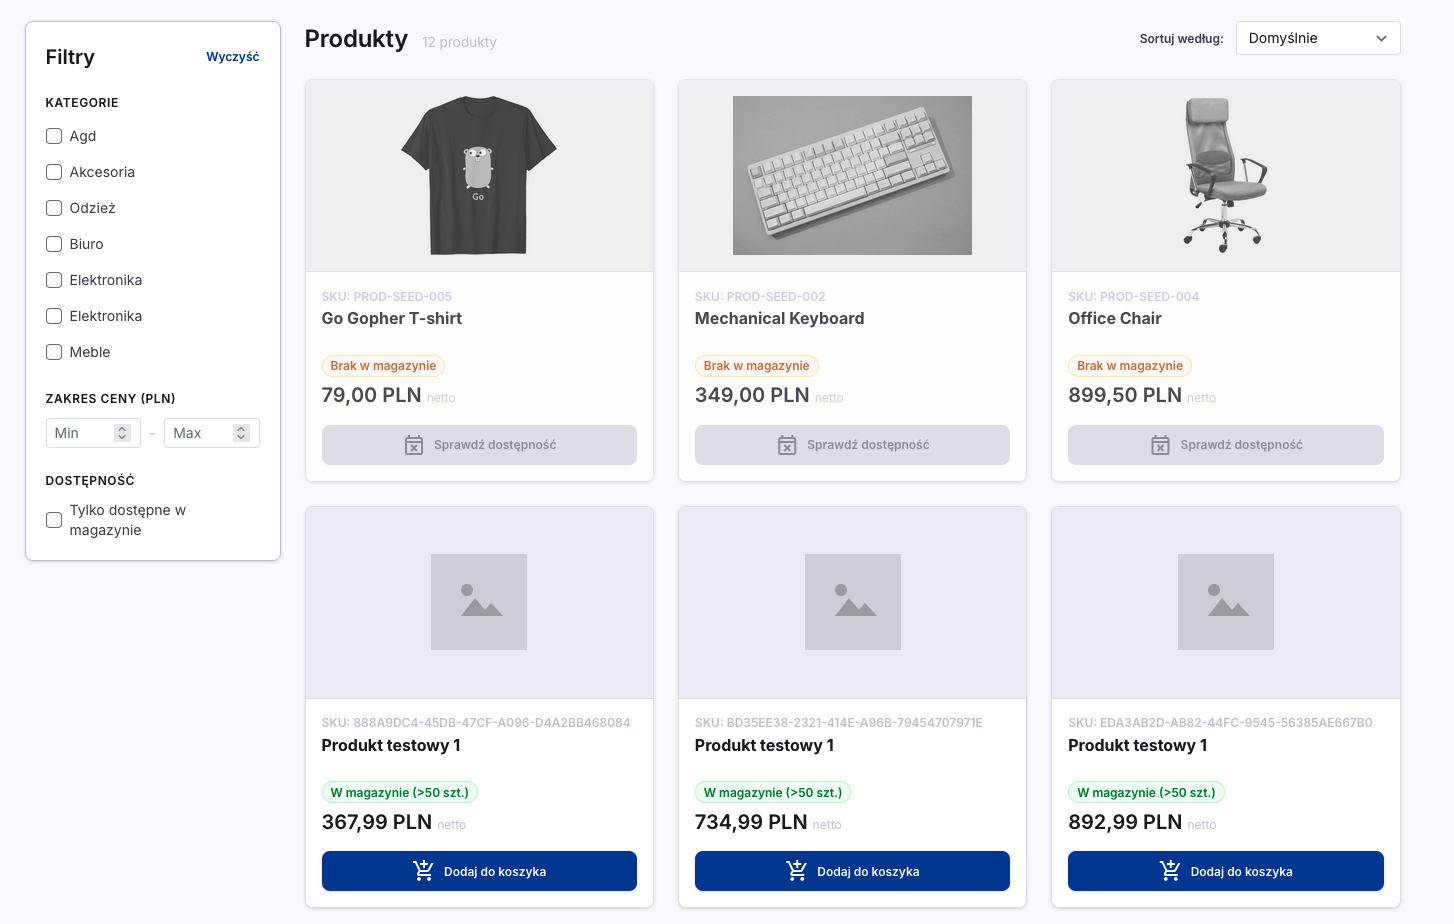
\includegraphics[width=\textwidth]{ProductView.png}
    \caption{Widok katalogu produktów zrealizowanego serwisu. (źródło: opracowanie własne)}
    \label{fig:product-view}
\end{figure}

\textbf{Koszyk} (\code{CartView}, rysunek~\ref{fig:cart-view}) umożliwia edycję ilości i~usuwanie pozycji
oraz na~bieżąco przelicza wartość zamówienia na~podstawie aktualnych cen z~katalogu.

\begin{figure}[H]
    \centering
    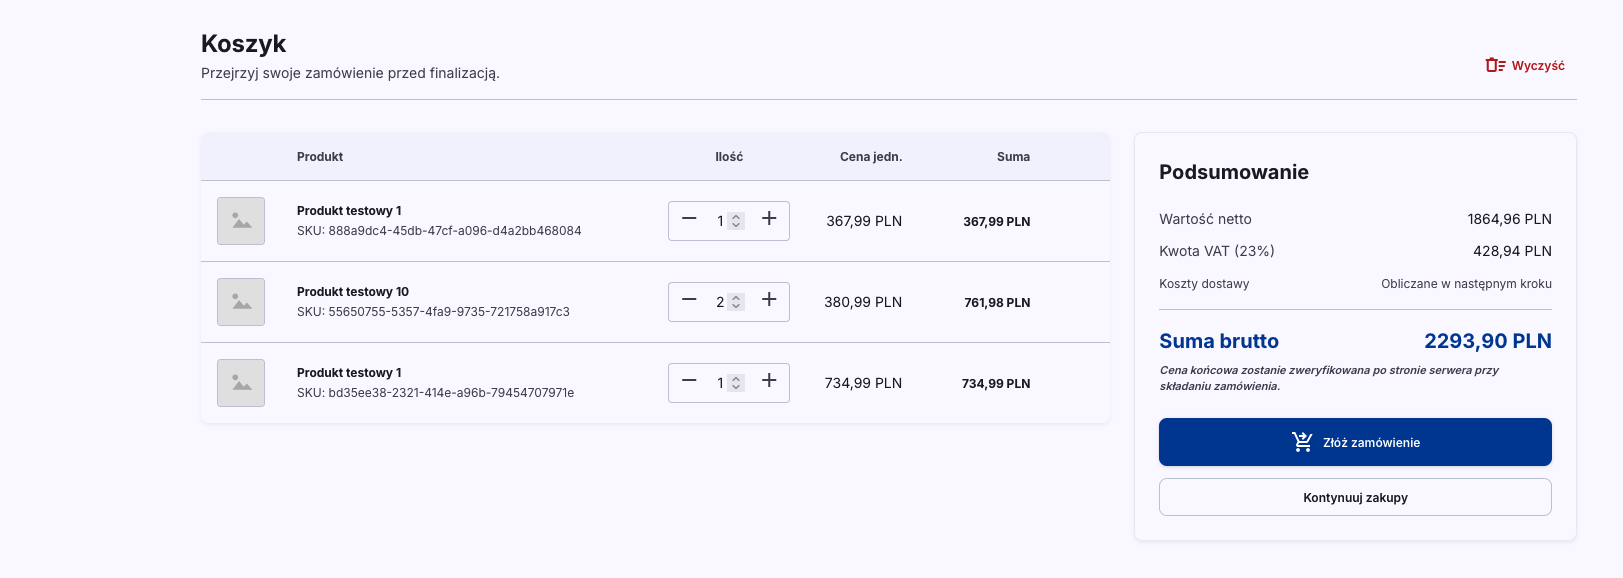
\includegraphics[width=\textwidth]{CartView.png}
    \caption{Widok koszyka zrealizowanego serwisu. (źródło: opracowanie własne)}
    \label{fig:cart-view}
\end{figure}

\textbf{Finalizacja} (\code{CheckoutView}) zbiera adres dostawy i~składa zamówienie; jej widok
przedstawiono na~rysunku~\ref{fig:checkout-view}.

\begin{figure}[H]
    \centering
    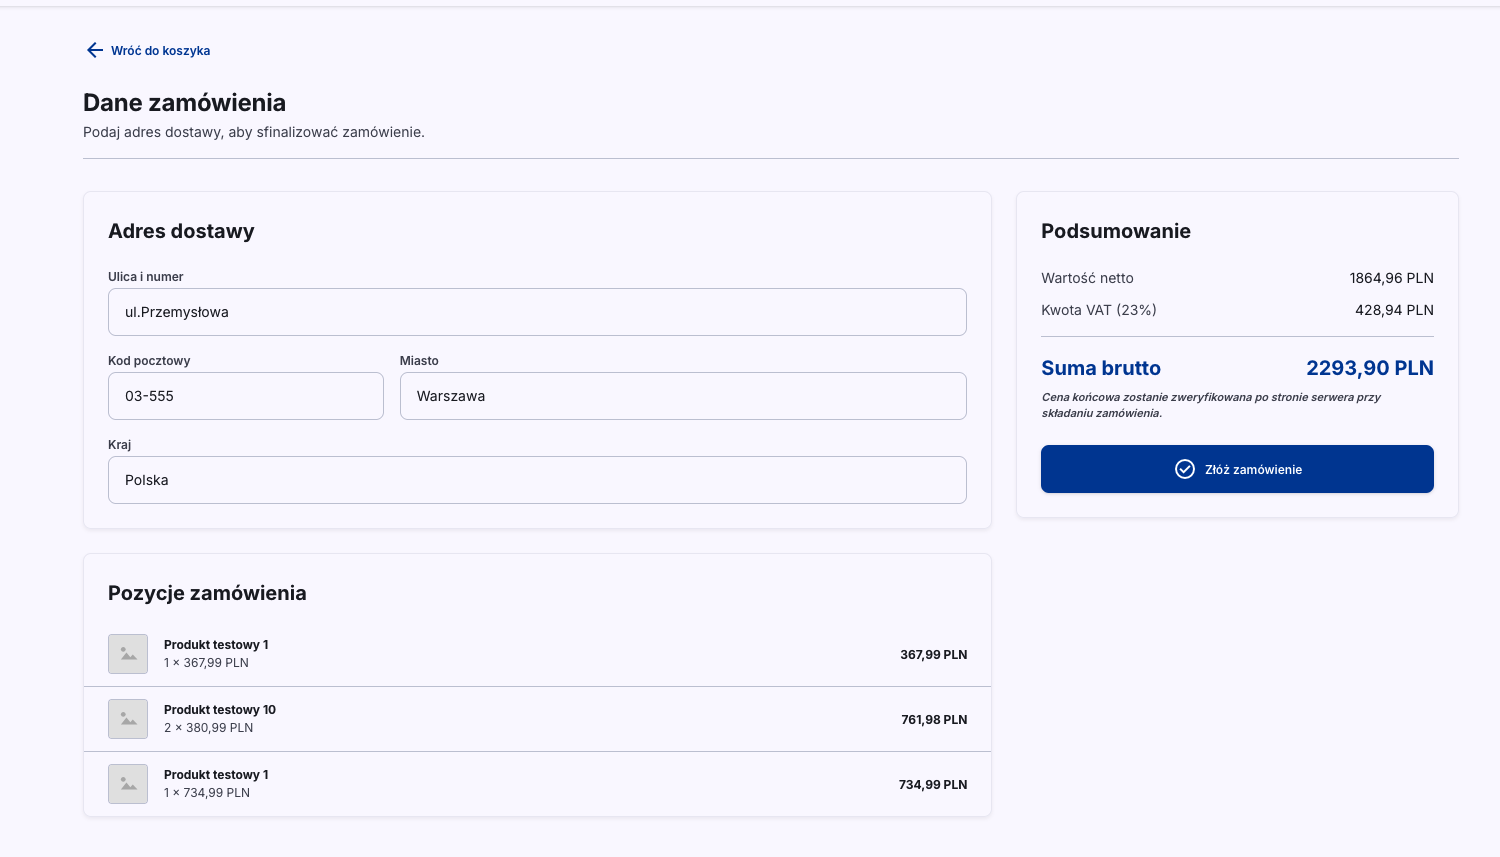
\includegraphics[width=\textwidth]{CheckoutView.png}
    \caption{Widok finalizacji zamówienia zrealizowanego serwisu. (źródło: opracowanie własne)}
    \label{fig:checkout-view}
\end{figure}

Po jego utworzeniu użytkownik przechodzi do \textbf{szczegółów zamówienia} (\code{OrderDetailsView}~).
Prezentujących pozycje, adres, bieżący status wraz z~wizualizacją postępu w~cyklu życia. Widok ten
przedstawiono na~rysunku~\ref{fig:order-details-view}.

\begin{figure}[H]
    \centering
    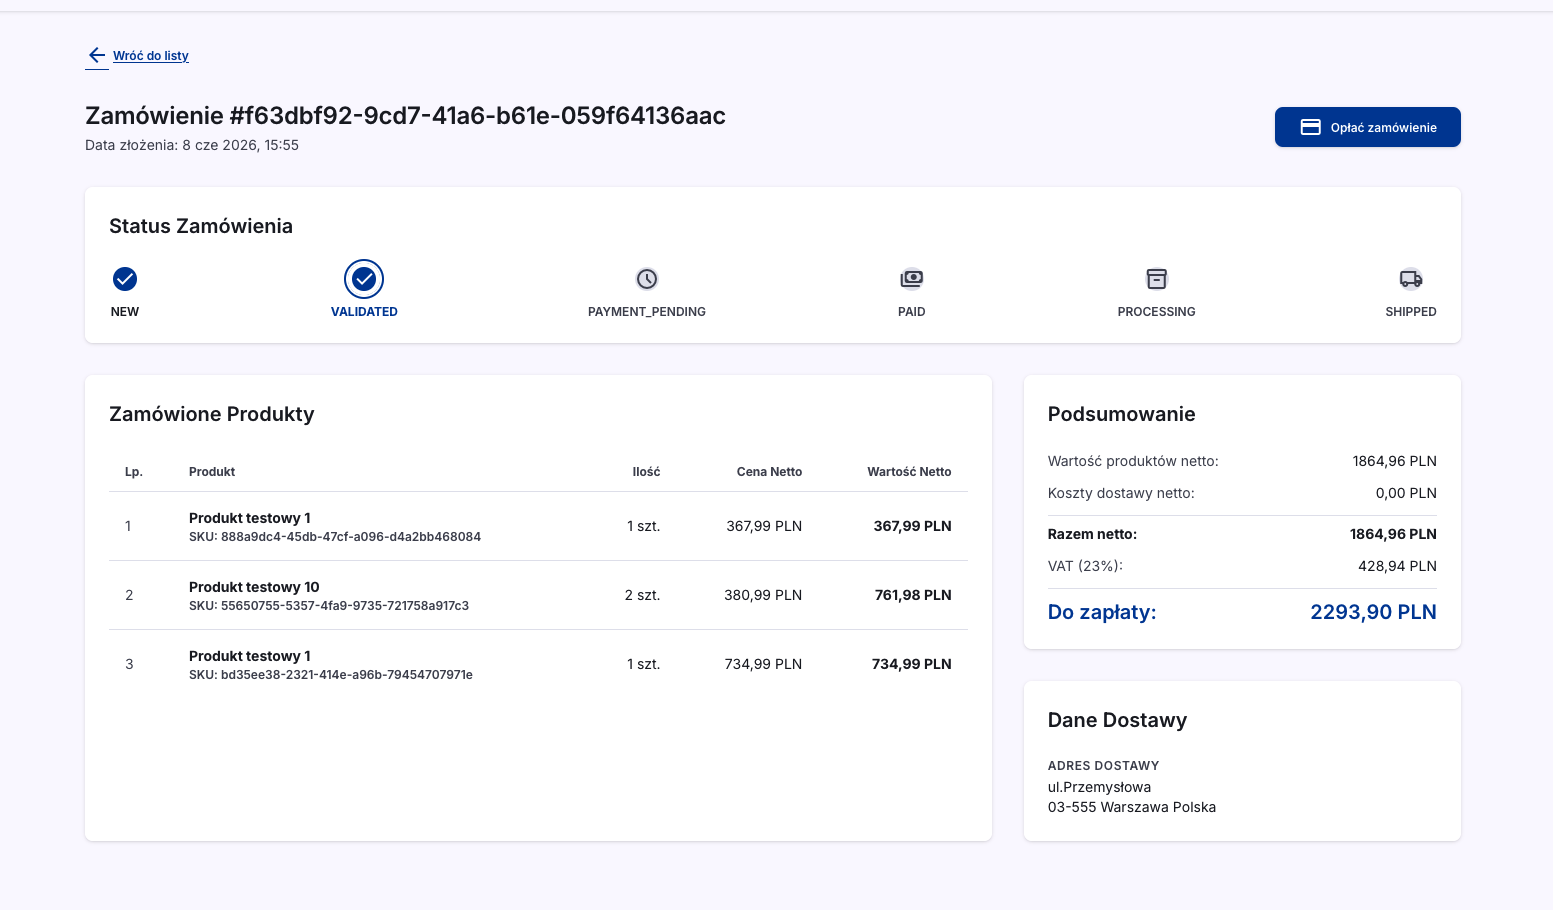
\includegraphics[width=\textwidth]{OrderDetailsView.png}
    \caption{Widok szczegółów zamówienia zrealizowanego serwisu. (źródło: opracowanie własne)}
    \label{fig:order-details-view}
\end{figure}

Przycisk rozpoczęcia płatności prowadzi do \textbf{widoku płatności} (\code{PaymentView}) z~symulowanym formularzem zapłaty,
który przedstawiono na~rysunku~\ref{fig:payment-view}.

\begin{figure}[H]
    \centering
    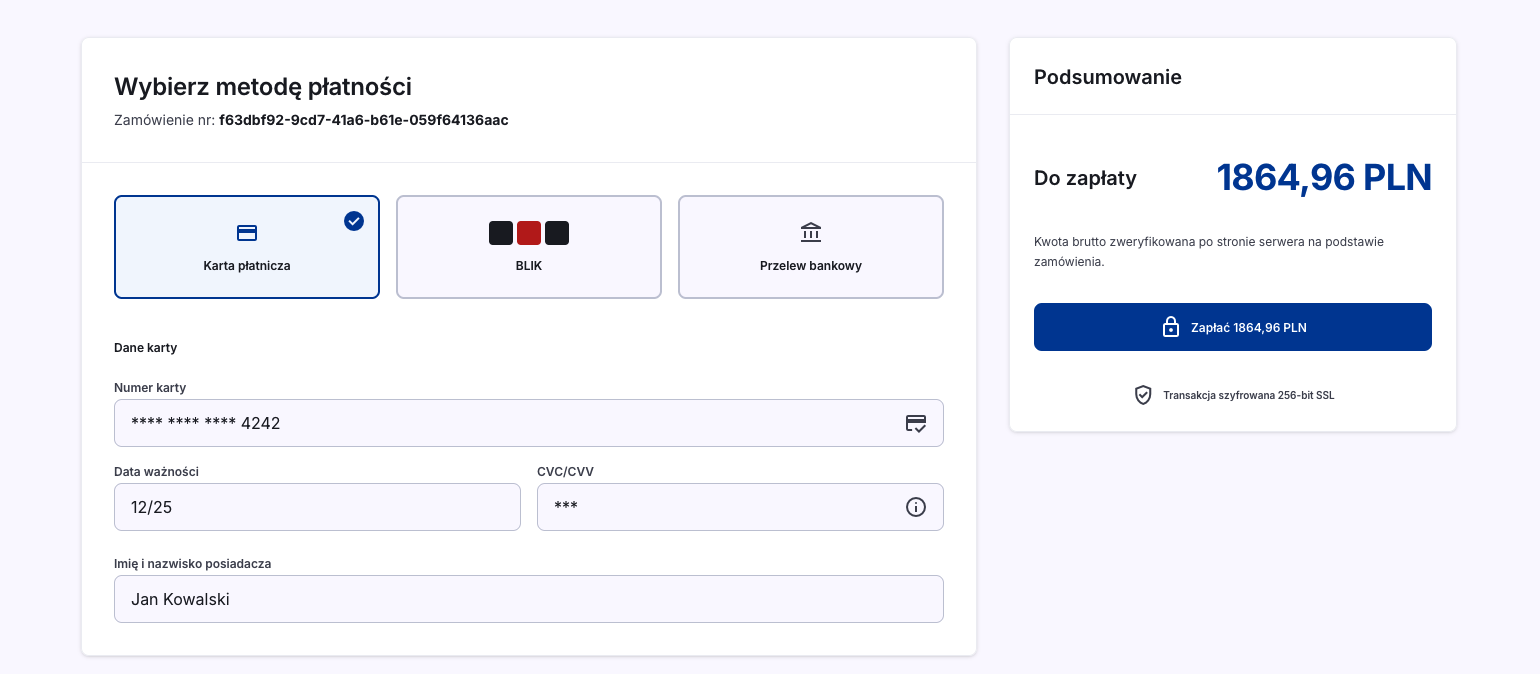
\includegraphics[width=\textwidth]{PaymentView.png}
    \caption{Widok płatności zrealizowanego serwisu. (źródło: opracowanie własne)}
    \label{fig:payment-view}
\end{figure}

Historię zamówień prezentuje \code{OrdersView} (rysunek~\ref{fig:order-history-view}), grupując zamówienia
według statusu i~umożliwiając przejście do~ich szczegółów.

\begin{figure}[H]
    \centering
    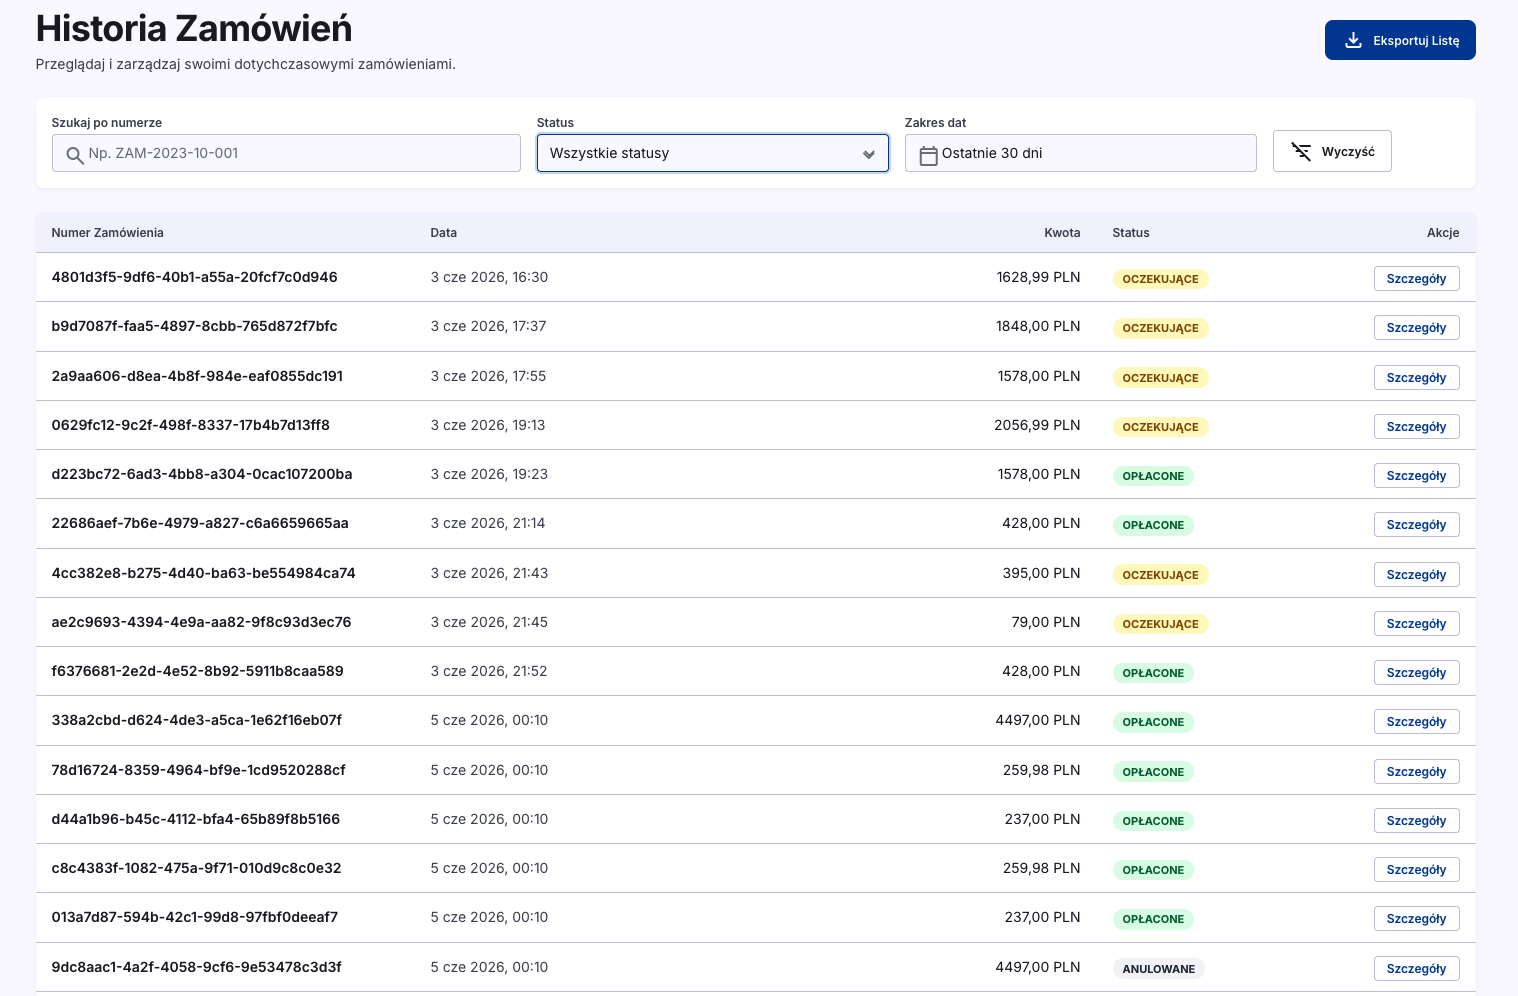
\includegraphics[width=\textwidth]{OrderHistory.png}
    \caption{Widok historii zamówień zrealizowanego serwisu. (źródło: opracowanie własne)}
    \label{fig:order-history-view}
\end{figure}

\textbf{Pulpit} (\code{DashboardView}) pokazuje podsumowanie, czyli liczbę aktywnych zamówień
i~ostatnią płatność; jego widok przedstawiono na~rysunku~\ref{fig:dashboard-view}.

\begin{figure}[H]
    \centering
    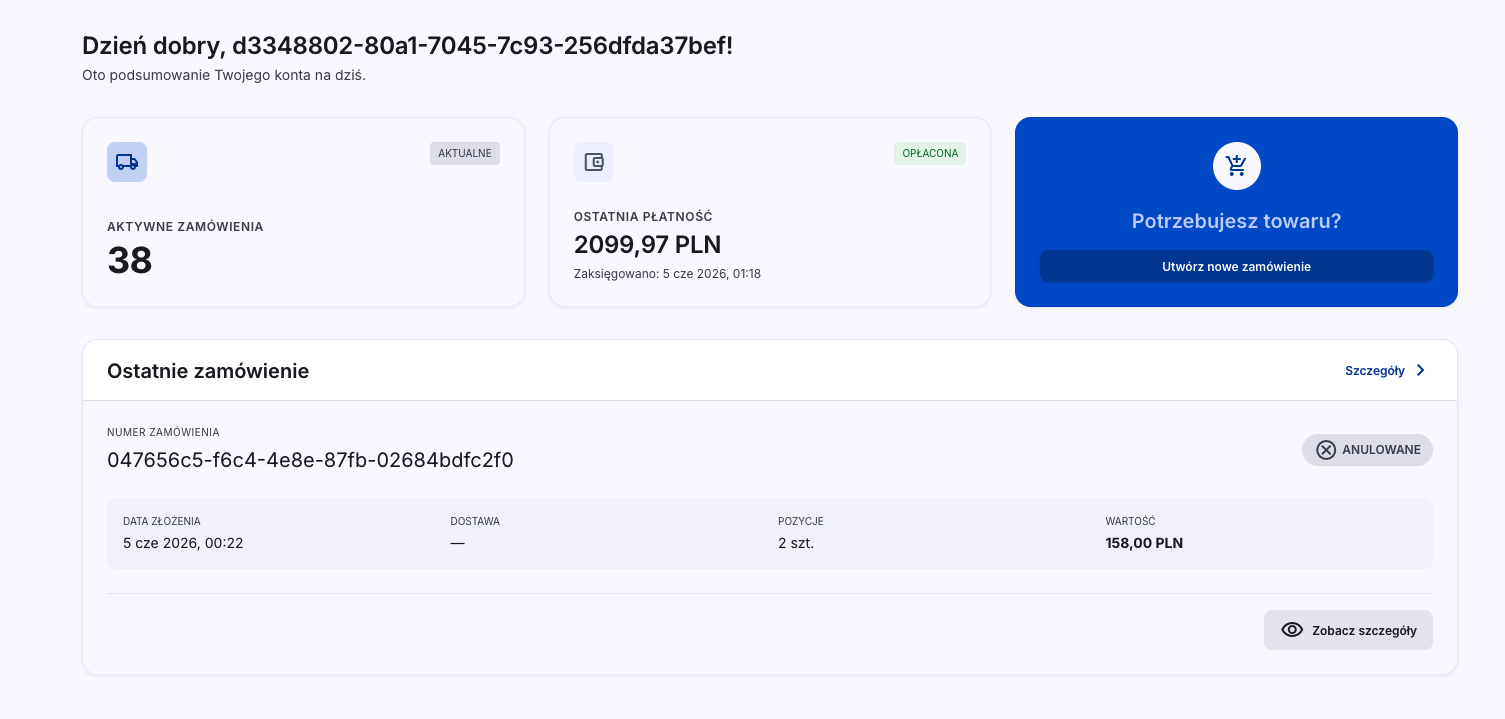
\includegraphics[width=\textwidth]{DashboardView.png}
    \caption{Widok pulpitu zrealizowanego serwisu. (źródło: opracowanie własne)}
    \label{fig:dashboard-view}
\end{figure}

Całość spina powłoka aplikacji ze~stałym panelem nawigacyjnym, który przedstawiono na~rysunku~\ref{fig:navigation-panel}.

\begin{figure}[H]
    \centering
    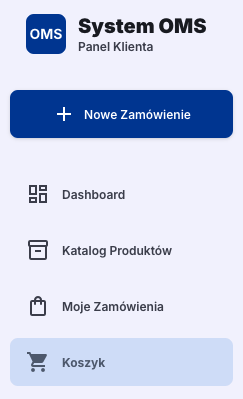
\includegraphics[scale=0.6]{NavigationPanel.png}
    \caption{Widok paneluj nawigacyjnego. (źródło: opracowanie własne)}
    \label{fig:navigation-panel}
\end{figure}

\section{Warstwa komunikacji z API}
\label{sec:warstwa-komunikacji-api}

Implementacje HTTP oparto na natywnym interfejsie \code{fetch}, bez zewnętrznych bibliotek. Odpowiedzi backendu
mapowane są na jawnie zadeklarowane typy aplikacji. Błędy mapowane są na komunikaty czytelne dla użytkownika. Nagłówki
uwierzytelniające dostarcza wstrzykiwana funkcja zwrotna powiązana z~dostawcą tożsamości, dzięki czemu warstwa
HTTP nie zna szczegółów mechanizmu logowania. Składanie zamówienia generuje po stronie przeglądarki klucz
idempotencji (listing~\ref{lst:create-order-http}), współpracując z~mechanizmem opisanym w~sekcji~\ref{sec:order-service}.

\begin{lstlisting}[caption={Złożenie zamówienia z kluczem idempotencji (fragment http.ts)},label={lst:create-order-http}]
async create(req: CreateOrderRequest): Promise<OrderDetail> {
  const res = await fetch(this.basePath, {
    method: 'POST',
    headers: {
      Accept: 'application/json',
      'Content-Type': 'application/json',
      'Idempotency-Key': crypto.randomUUID(),
      ...this.authHeaders(),
    },
    body: JSON.stringify(body),
  })
  if (!res.ok) throw new Error(`Nie udalo sie zlozyc zamowienia (HTTP ${res.status}).`)
  return toOrderDetail((await res.json()) as BackendOrder)
}
\end{lstlisting}

Adresy API są względne (\code{/api/orders}, \code{/api/products}, \code{/api/v1/payments}). Portal nie zna
topologii backendu, a~rozdziałem żądań pomiędzy mikroserwisy zajmuje się warstwa brzegowa systemu
(rozdział~\ref{chap:infrastruktura}). Eliminuje to problemy współdzielenia zasobów między domenami (CORS).

\section{Logowanie użytkownika - OAuth 2.0 z PKCE}
\label{sec:logowanie-pkce}

Logowanie zaimplementowano zgodnie z~projektem przedstawionym w~sekcji~\ref{sec:projekt-uwierzytelniania}.
W~przepływie \emph{authorization code} z~rozszerzeniem PKCE, wobec hostowanego interfejsu logowania Cognito.
Rozpoczynając logowanie, aplikacja generuje kryptograficznie losowy weryfikator oraz jego skrót SHA-256
(listing~\ref{lst:pkce-helpers}), korzystając wyłącznie z~natywnych interfejsów Web Crypto. Bez zewnętrznych
bibliotek kryptograficznych. Weryfikator, wraz z~losowym parametrem \code{state} (chroniącym przed atakami CSRF)
i~docelową trasą po zalogowaniu, zapisywany jest w~\code{sessionStorage}. Po czym przeglądarka przekierowywana
jest na punkt końcowy autoryzacji Cognito z~parametrami \code{code\_challenge} i~\code{code\_challenge\_method=S256}.
Punktem wejścia dla~niezalogowanego użytkownika jest strona startowa z~przyciskiem logowania
(rysunek~\ref{fig:home-view}), kierująca do~hostowanego formularza logowania Cognito
(rysunek~\ref{fig:cognito-login-view}), na~którym następuje właściwe uwierzytelnienie.

\begin{figure}[H]
    \centering
    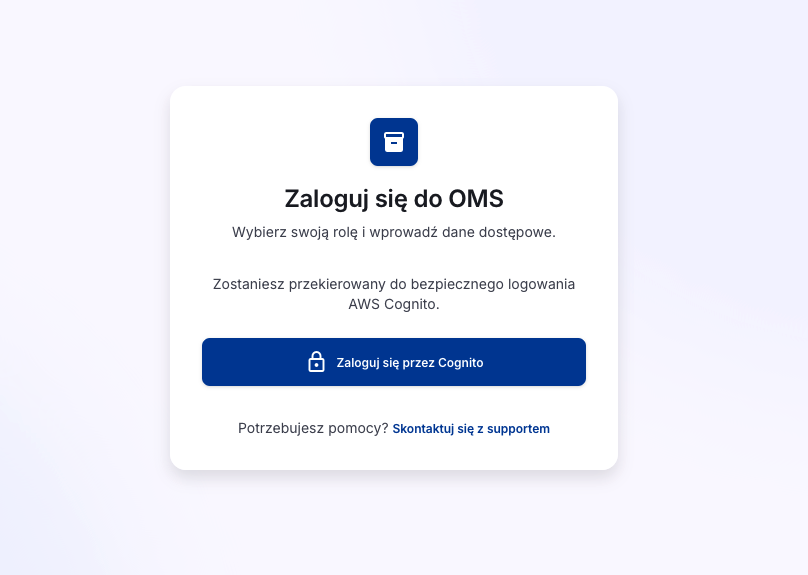
\includegraphics[scale=0.6]{HomeView.png}
    \caption{Widok strony przekierowującej do logowania. (źródło: opracowanie własne)}
    \label{fig:home-view}
\end{figure}


\begin{figure}[H]
    \centering
    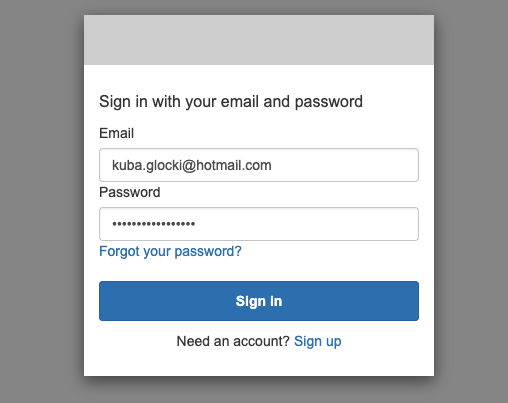
\includegraphics[scale=0.6]{CognitoLogin.png}
    \caption{Widok logowania Cognito. (źródło: opracowanie własne)}
    \label{fig:cognito-login-view}
\end{figure}

\begin{lstlisting}[caption={Generowanie weryfikatora i wyzwania PKCE (Web Crypto)},label={lst:pkce-helpers}]
function randomString(byteLength: number): string {
  const bytes = new Uint8Array(byteLength)
  crypto.getRandomValues(bytes)
  return base64UrlEncode(bytes)
}

async function pkceChallenge(verifier: string): Promise<string> {
  const digest = await crypto.subtle.digest(
    'SHA-256',
    new TextEncoder().encode(verifier),
  )
  return base64UrlEncode(new Uint8Array(digest))
}
\end{lstlisting}

Po uwierzytelnieniu Cognito zwraca przeglądarkę na zarejestrowaną trasę zwrotną z~kodem autoryzacyjnym. Widok
\code{AuthCallbackView} weryfikuje zgodność parametru \code{state} z~zapamiętanym, a~następnie wymienia kod na
tokeny żądaniem POST do punktu \code{/oauth2/token}. Przedstawiając oryginalny weryfikator, co domyka
mechanizm PKCE. Otrzymane tokeny (identyfikacyjny, dostępowy i~odświeżający, wraz z~wyliczonym czasem wygaśnięcia)
zapisywane są w~\code{localStorage}. Dzięki czemu sesja przetrwa odświeżenie strony. Dane użytkownika odczytywane 
są z~ładunku tokenu identyfikacyjnego. Portal celowo nie weryfikuje podpisu tokenu. 
Właściwa weryfikacja kryptograficzna następuje w~każdym mikroserwisie przy każdym żądaniu
(sekcja~\ref{sec:implementacja-auth}). Bezpieczeństwo systemu nie opiera się więc na kodzie działającym
w~przeglądarce. Wylogowanie usuwa tokeny z~pamięci lokalnej i~przekierowuje na punkt końcowy wylogowania Cognito,
unieważniając również sesję po stronie dostawcy tożsamości.

Pełny przebieg tego procesu przedstawiono na~rysunku~\ref{fig:pkce} w~rozdziale~\ref{chap:projekt-systemu}.
\chapter{Budowa środowiska chmurowego --- infrastruktura jako kod}
\label{chap:infrastruktura}

Całość środowiska uruchomieniowego systemu zdefiniowano deklaratywnie w~narzędziu Terraform.
Środowisko jest w~pełni odtwarzalne. Pojedyncze wykonanie \code{terraform apply}
buduje je od zera, bez jakichkolwiek czynności ręcznych w~konsoli AWS. Rozdział omawia kolejne warstwy tej
infrastruktury w~porządku, w~jakim są tworzone. System uruchomiono w~regionie \code{eu-central-1} (Frankfurt).

\section{Terraform i zarządzanie stanem infrastruktury}
\label{sec:terraform-stan}

Terraform przechowuje stan infrastruktury. W pliku stanu odwzorowano zasoby zadeklarowane w~kodzie na zasoby istniejące
w~chmurze. W przypadku pracy zespołowej i~automatyzacji musi być składowany zdalnie. Wykorzystano, więc
backend S3. Stan trafia do dedykowanego bucketa z~włączonym wersjonowaniem (możliwość odtworzenia wcześniejszych
wersji stanu), szyfrowaniem oraz całkowitą blokadą dostępu publicznego. Równoległe modyfikacje wyklucza
mechanizm blokady plików.

Projekt wykorzystuje trzech dostawców. (\emph{Providers}) \code{aws} dla zasobów chmurowych. \code{Kubernetes}
dla obiektów wewnątrz klastra. \code{Random} do generowania sekretów.
Objęcie jednym narzędziem obu warstw pozwala wyrażać zależności pomiędzy nimi wprost w~kodzie. Manifesty Kubernetes 
odwołują się do atrybutów zasobów AWS. Kolejność tworzenia wyznacza graf zależności Terraform. 
Parametry środowiska wyniesiono do zmiennych z~wartościami w~pliku \code{terraform.tfvars}.
Dzięki czemu odtworzenie środowiska o~innych parametrach (np. większych instancjach)
sprowadza się do zmiany pliku zmiennych.

\section{Konfiguracja sieci VPC}
\label{sec:konfiguracja-vpc}

Sieć systemu obejmuje VPC o~adresacji \code{10.0.0.0/16}, rozpiętą na dwie strefy dostępności. W~każdej strefie
wydzielono po dwie podsieci \code{/24}.
Publiczną (\code{10.0.0.0/24}, \code{10.0.1.0/24}) oraz prywatną (\code{10.0.100.0/24}, \code{10.0.101.0/24}).
Podsieci publiczne posiadają trasę do bramy internetowej. Posiadają tylko elemety brzegowe: load balancer
oraz bramę NAT. W~podsieciach prywatnych działają węzły klastra i~baza danych, których ruch wychodzący
kierowany jest przez NAT (rysunek~\ref{fig:topologia-sieci}). Ze~względów kosztowych zastosowano pojedynczą bramę NAT.

Podsieci opatrzono tagami, którymi posługuje się integracja Kubernetes z~AWS przy wyborze podsieci dla load
balancerów (listing~\ref{lst:vpc-tagi}). Filtrowanie ruchu realizują grupy bezpieczeństwa opisane
w~sekcji~\ref{sec:routing-ruchu}.

\begin{lstlisting}[caption={Definicja podsieci prywatnych z tagami Kubernetes (vpc.tf)},label={lst:vpc-tagi}]
resource "aws_subnet" "private" {
  count             = length(local.azs)
  vpc_id            = aws_vpc.this.id
  cidr_block        = cidrsubnet(var.vpc_cidr, 8, count.index + 100)
  availability_zone = local.azs[count.index]

  tags = {
    Name                                          = "${local.name}-private-${local.azs[count.index]}"
    "kubernetes.io/role/internal-elb"             = "1"
    "kubernetes.io/cluster/${local.cluster_name}" = "shared"
  }
}
\end{lstlisting}

\begin{figure}[H]
    \centering
    \begin{tikzpicture}[
        font=\scriptsize,
        >={Stealth[length=1.6mm]},
        box/.style={rectangle, rounded corners, draw, thick, align=center,
                    minimum height=6mm, minimum width=20mm},
        pub/.style={box, fill=black!4},
        priv/.style={box, fill=black!10},
        sub/.style={rectangle, draw, densely dashed, inner sep=3mm, rounded corners},
    ]
        \node[box, fill=black!3] (igw) {Internet Gateway};

        % AZ A
        \node[pub, below left=10mm and 2mm of igw] (alba) {ALB / NAT};
        \node[priv, below=8mm of alba] (nodea) {Węzły EKS};
        \node[priv, below=6mm of nodea] (rdsa) {RDS (primary)};
        \begin{scope}[on background layer]
            \node[sub, fill=black!2, fit=(alba)] (pubA) {};
            \node[sub, fill=black!6, fit=(nodea)(rdsa)] (privA) {};
        \end{scope}

        % AZ B
        \node[pub, below right=10mm and 2mm of igw] (albb) {NAT (zapas)};
        \node[priv, below=8mm of albb] (nodeb) {Węzły EKS};
        \node[priv, below=6mm of nodeb] (rdsb) {RDS (standby)};
        \begin{scope}[on background layer]
            \node[sub, fill=black!2, fit=(albb)] (pubB) {};
            \node[sub, fill=black!6, fit=(nodeb)(rdsb)] (privB) {};
        \end{scope}

        \node[font=\scriptsize\itshape, above=1mm of pubA] {strefa A};
        \node[font=\scriptsize\itshape, above=1mm of pubB] {strefa B};
        \node[font=\scriptsize, left=1mm of pubA] {publ.};
        \node[font=\scriptsize, left=1mm of privA] {pryw.};

        \draw[->, thick] (igw) -- (alba);
        \draw[->, thick] (igw) -- (albb);
        \draw[->, thick] (alba) -- (nodea);
        \draw[->, thick, densely dashed] (nodea) -- (rdsa);
        \draw[->, thick, densely dashed] (nodeb) -- (rdsb);

        \begin{scope}[on background layer]
            \node[sub, draw=black!50, fit=(igw)(pubA)(privA)(pubB)(privB),
                  inner sep=5mm, label={[font=\scriptsize\bfseries]above:VPC 10.0.0.0/16}] {};
        \end{scope}
    \end{tikzpicture}
    \caption{Topologia sieci VPC. Komponenty brzegowe (ALB, bramy NAT) działają w~podsieciach publicznych, a~węzły klastra i~baza danych --- w~prywatnych, pozbawionych bezpośredniej łączności z~Internetem. Zasoby rozmieszczono w~dwóch strefach dostępności. Baza danych w~środowisku pracuje jednostrefowo; wariant standby zaznaczono jako~opcję trybu Multi-AZ.}
    \label{fig:topologia-sieci}
\end{figure}

\section{Utworzenie klastra EKS i grup węzłów}
\label{sec:utworzenie-eks}

Klaster EKS utworzono z~płaszczyzną sterowania rozpiętą na podsieci prywatne obu stref
dostępności. Uprawnienia administracyjne do klastra nadawane są wpisami
dostępu powiązanymi z~tożsamościami IAM, bez ręcznej edycji map konfiguracyjnych wewnątrz klastra.

\begin{figure}[H]
    \centering
    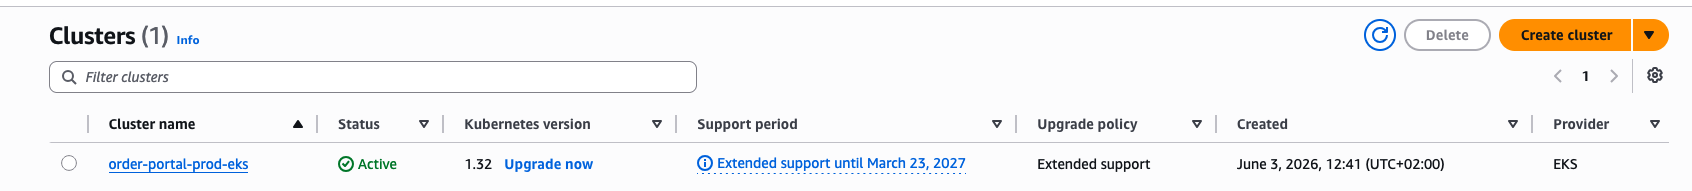
\includegraphics[width=\textwidth]{ClusterEKS.png}
    \caption{Konsola Amazon EKS: klaster \code{order-portal-prod-eks} w~wersji Kubernetes~1.32, w~stanie aktywnym.}
    \label{fig:cluster-eks}
\end{figure}

Warstwę obliczeniową stanowi zarządzana grupa węzłów. Cztery instancje \code{t3.small} (2~vCPU, 2~GiB RAM każda)
z~obrazem AL2023, w~trybie \emph{on-demand}, z~dyskami 20~GiB, rozmieszczane w~podsieciach prywatnych. Aktualizacje
grupy przebiegają z~ograniczeniem \code{max\_unavailable = 1}, czyli wymianą najwyżej jednego węzła naraz. Dla tak
małych instancji krytyczna okazała się konfiguracja wtyczki sieciowej VPC CNI (listing~\ref{lst:prefix-delegation}).
Domyślnie liczba podów na węźle ograniczona jest pulą adresów IP interfejsów sieciowych instancji
co uniemożliwiłoby zmieszczenie wszystkich komponentów systemu wraz z~podami systemowymi. Włączenie delegacji 
prefiksów (\code{ENABLE\_PREFIX\_DELEGATION}) przydziela interfejsom całe prefiksy \code{/28} zamiast pojedynczych adresów, podnosząc limit wielokrotnie.

\begin{lstlisting}[caption={Dodatek VPC CNI z delegacją prefiksów (eks.tf)},label={lst:prefix-delegation}]
resource "aws_eks_addon" "vpc_cni" {
  cluster_name                = aws_eks_cluster.this.name
  addon_name                  = "vpc-cni"
  resolve_conflicts_on_create = "OVERWRITE"
  resolve_conflicts_on_update = "OVERWRITE"

  configuration_values = jsonencode({
    env = {
      ENABLE_PREFIX_DELEGATION = "true"
      WARM_PREFIX_TARGET       = "1"
    }
  })
}
\end{lstlisting}

\begin{figure}[H]
    \centering
    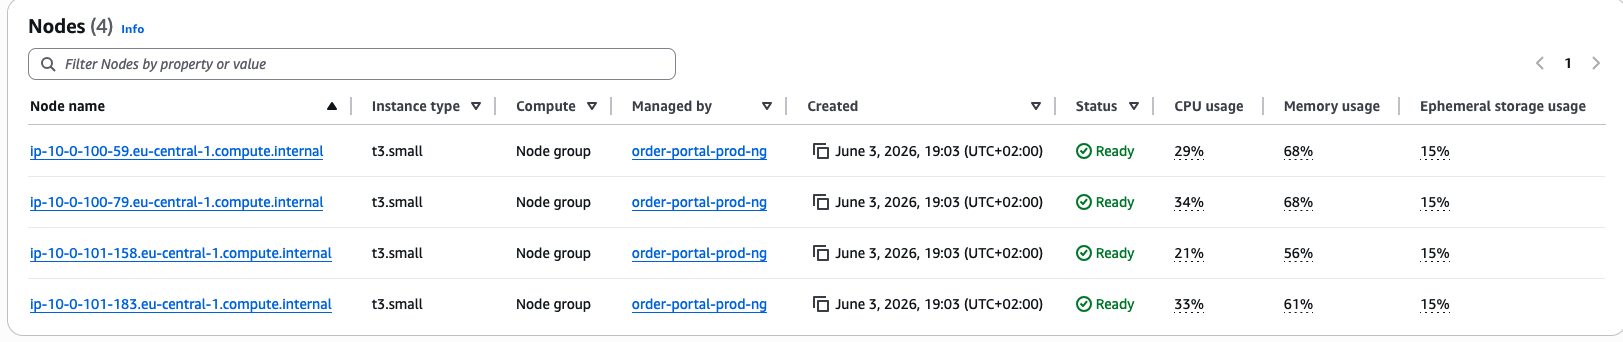
\includegraphics[width=\textwidth]{NodesEKS.png}
    \caption{Cztery węzły grupy \code{order-portal-prod-ng} (instancje \code{t3.small}) w~stanie \emph{Ready}. Wykorzystanie pamięci (56--68\%) wyraźnie przewyższa wykorzystanie procesora (21--34\%) --- co~potwierdza ustalenie z~rozdziału~\ref{chap:testy-i-analiza}, że~to~pamięć, a~nie~procesor, jest~czynnikiem ograniczającym gęstość podów.}
    \label{fig:nodes-eks}
\end{figure}

Funkcjonalność klastra dopełniają zarządzane dodatki (\emph{add-ons}). Są to komponenty systemowe instalowane
i~aktualizowane przez EKS, lecz działające jako zwykłe pody wewnątrz klastra. W~zrealizowanym systemie
wykorzystano cztery takie dodatki. \code{CoreDNS} pełni rolę wewnętrznego serwera DNS klastra. To dzięki niemu
mikroserwisy odnajdują się nawzajem po~stabilnych nazwach (np. \code{order-service}) zamiast po~zmiennych adresach
IP podów. \code{kube-proxy} programuje na~każdym węźle reguły sieciowe realizujące obiekty Service, czyli
kierujące ruch z~nazwy usługi do~jej aktualnych replik. Agent \textbf{EKS Pod Identity} umożliwia nadawanie podom
uprawnień do~usług AWS. Sterownik \textbf{EBS CSI} odpowiada za~trwałe składowanie danych: na~żądanie aplikacji
(obiekt PersistentVolumeClaim) automatycznie tworzy w~AWS wolumin EBS i~podłącza go do~poda.

\begin{figure}[H]
    \centering
    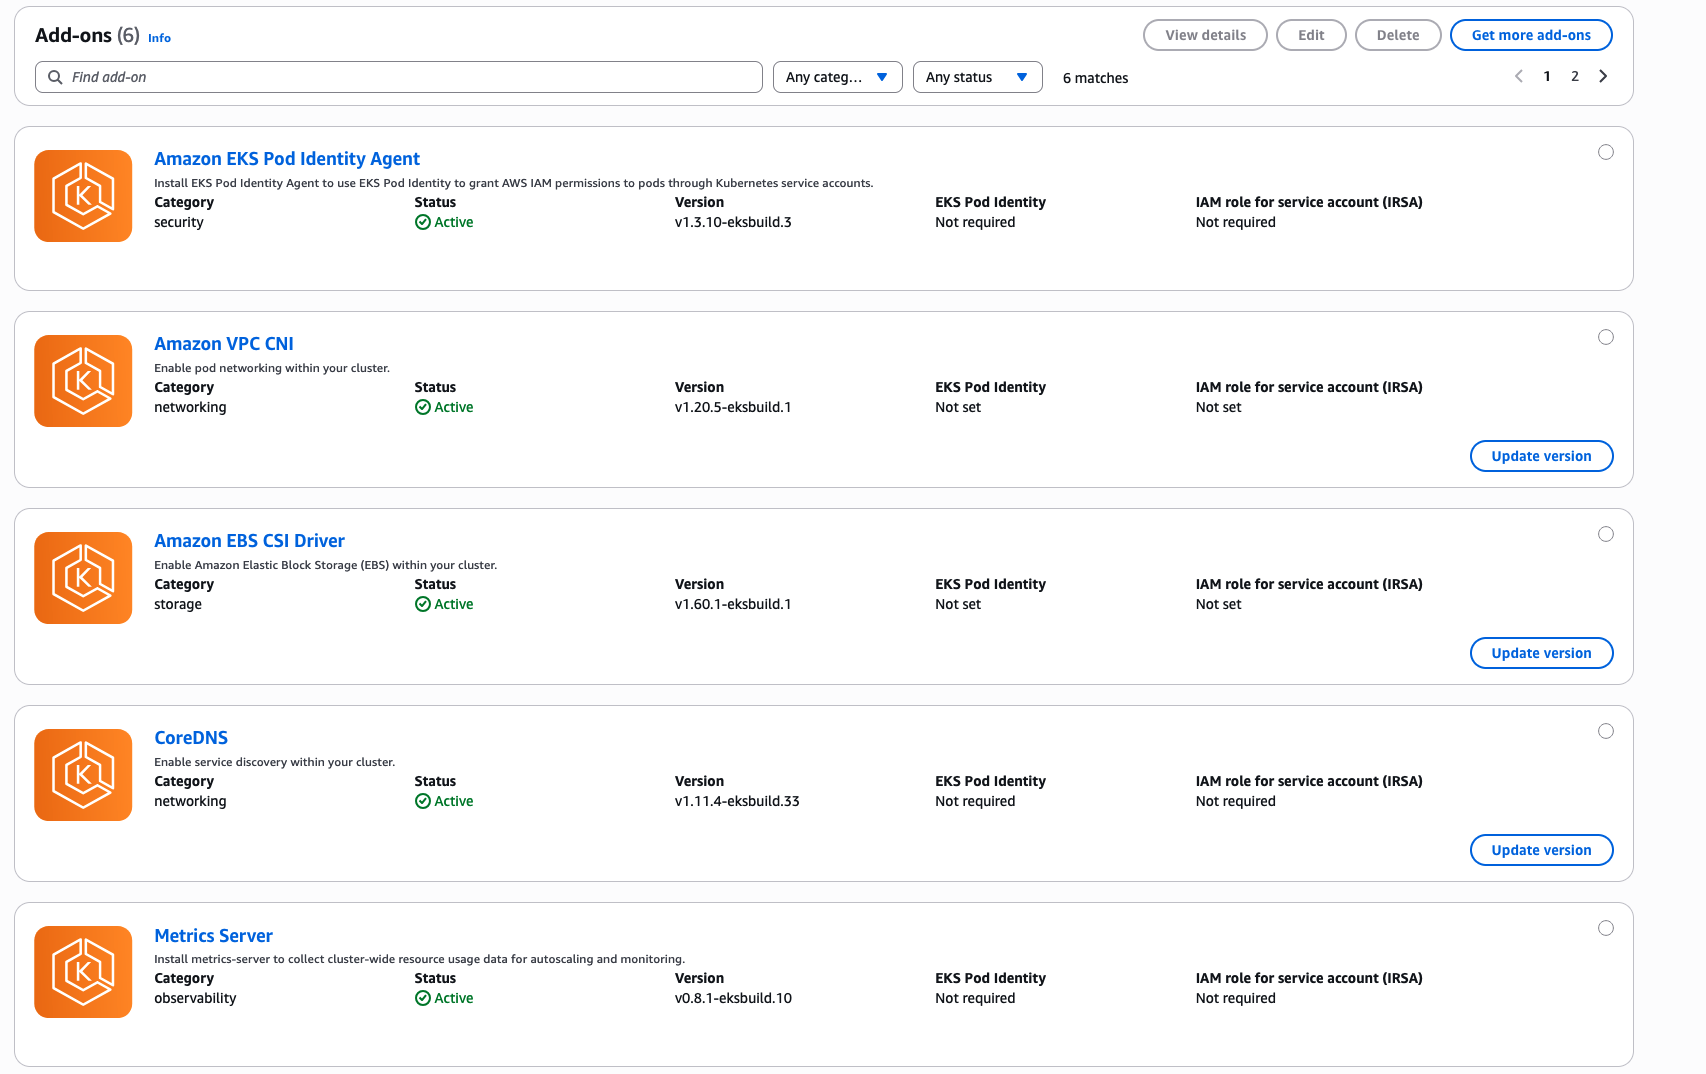
\includegraphics[width=\textwidth]{AddonsEKS.png}
    \caption{Zarządzane dodatki klastra EKS --- agent Pod Identity, VPC CNI, sterownik EBS CSI, CoreDNS oraz metrics-server --- wszystkie w~stanie aktywnym.}
    \label{fig:addons-eks}
\end{figure}

Sterownik EBS CSI, aby tworzyć woluminy, musi mieć uprawnienia do~odpowiednich operacji w~API AWS.
KLonto usługi sterownika powiązano mechanizmem Pod Identity z~dedykowaną
rolą IAM o~minimalnym zakresie uprawnień (sekcja~\ref{sec:bezpieczenstwo-kubernetes}). Dzięki temu sterownik
otrzymuje automatycznie rotowane poświadczenia krótkoterminowe, których ewentualny wyciek ma znikome konsekwencje,
a~w~repozytorium ani w~obrazach kontenerów nie~przechowuje się żadnych trwałych kluczy.

Na~potrzeby woluminów trwałych zdefiniowano klasę pamięci, wskazującą
sterownikowi, jakie woluminy tworzyć. Są~to woluminy typu gp3, szyfrowane w~spoczynku, z~możliwością późniejszego
powiększenia. Zastosowano tryb wiązania \emph{WaitForFirstConsumer}. Utworzenie woluminu jest~wstrzymywane do~chwili,
aż~Kubernetes zdecyduje, na~którym węźle uruchomić korzystający z~niego pod. Ma~to istotne znaczenie w~środowisku
wielostrefowym. Wolumin EBS jest~przypisany do~jednej strefy dostępności i~nie~może być~podłączony do~poda
działającego w~innej. Odroczenie utworzenia woluminu gwarantuje, że~powstanie on~w~tej~samej strefie, co~pod,
który ma~go używać.

\section{Warstwa danych --- RDS PostgreSQL i Secrets Manager}
\label{sec:warstwa-danych-rds}

Bazę danych utworzono jako instancję RDS PostgreSQL~18 klasy \code{db.t4g.micro} z~20~GiB szyfrowanego składowania gp3.
Wytworzono go w~podsieciach prywatnych. Dostęp sieciowy ogranicza dedykowana grupa
bezpieczeństwa, przepuszczająca port 5432 wyłącznie z~grupy bezpieczeństwa węzłów klastra. Baza nie jest
osiągalna ani z~Internetu, ani z~podsieci publicznych. W~środowisku przyjęto jednodniową retencję kopii zapasowych
i~tryb jednostrefowy.

\begin{figure}[H]
    \centering
    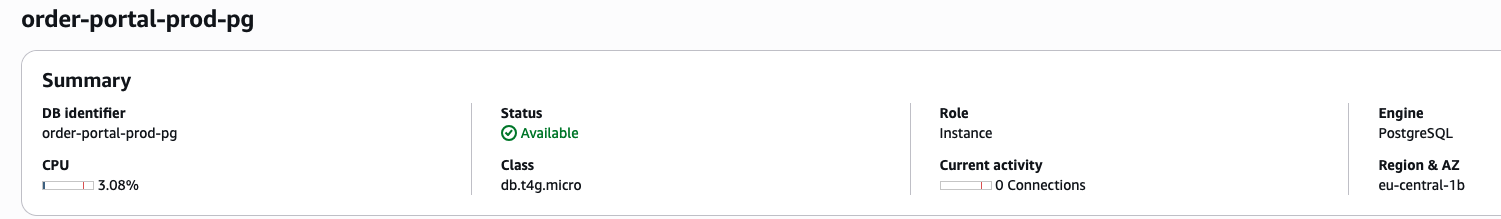
\includegraphics[width=\textwidth]{PosgreSQL.png}
    \caption{Konsola Amazon RDS: instancja PostgreSQL \code{order-portal-prod-pg} klasy \code{db.t4g.micro} w~strefie \code{eu-central-1b}, w~stanie dostępnym.}
    \label{fig:postgreSQL-RDS}
\end{figure}

Hasło użytkownika bazy generowane jest zasobem \code{random\_password} i nie występuje w~kodzie źródłowym.
Komplet poświadczeń zapisywany jest w~usłudze Secrets Manager.

\section{Wdrożenie mikroserwisów i brokera Kafka do klastra}
\label{sec:wdrozenie-do-klastra}

Komponenty aplikacyjne działają w~dedykowanej przestrzeni nazw \code{order-portal}. Deploymenty trzech
mikroserwisów generowane są z~jednej definicji. Pętlą po mapie usług. Zasoby serwisów ograniczono do 100m~CPU / 128~MiB żądanie i~500m~CPU / 512~MiB limit.

Konfiguracja każdej usługi składana jest w~Terraformie do pliku \code{.env}, przechowywanego jako Secret i~montowanego 
do kontenera jako wolumin tylko do odczytu. Szablony wdrożeniowe niosą również adnotacje
\code{prometheus.io/scrape}, \code{prometheus.io/port} i~\code{prometheus.io/path}, włączające pody do monitoringu
(sekcja~\ref{sec:wdrozenie-monitoringu}). Każdej usłudze towarzyszy obiekt Service typu ClusterIP, udostępniający
ją pod stabilną nazwą DNS.

\begin{figure}[H]
    \centering
    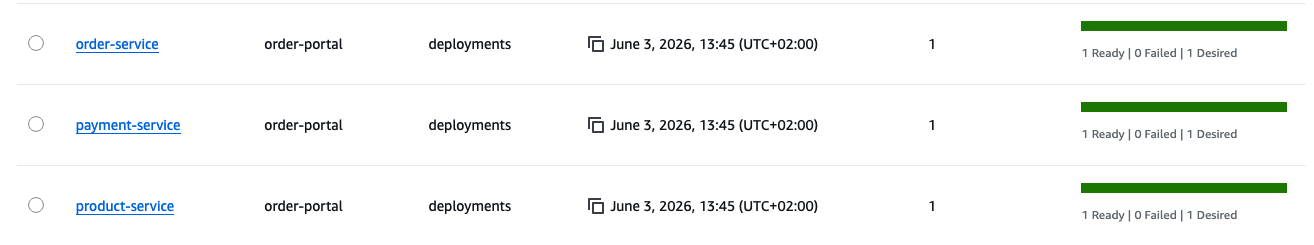
\includegraphics[width=\textwidth]{ServicesEKS.png}
    \caption{Trzy mikroserwisy wdrożone w~przestrzeni nazw \code{order-portal} jako obiekty Deployment --- każdy w~stanie gotowości (1~Ready / 1~Desired).}
    \label{fig:serices-eks}
\end{figure}

Broker Kafka uruchomiono jako Deployment z~obrazem \code{apache/kafka:4.3.0}, Dziennik zdarzeń składowany jest na 
trwałym woluminie 5~GiB klasy \code{ebs-gp3}. Z tego powodu dane przetrwają
restart i~przeniesienie poda. Tematy \code{order.events} i~\code{product.events} tworzy jednorazowy Job inicjalizacyjny,
wykonujący narzędzie \code{kafka-topics} po starcie brokera.

\begin{figure}[H]
    \centering
    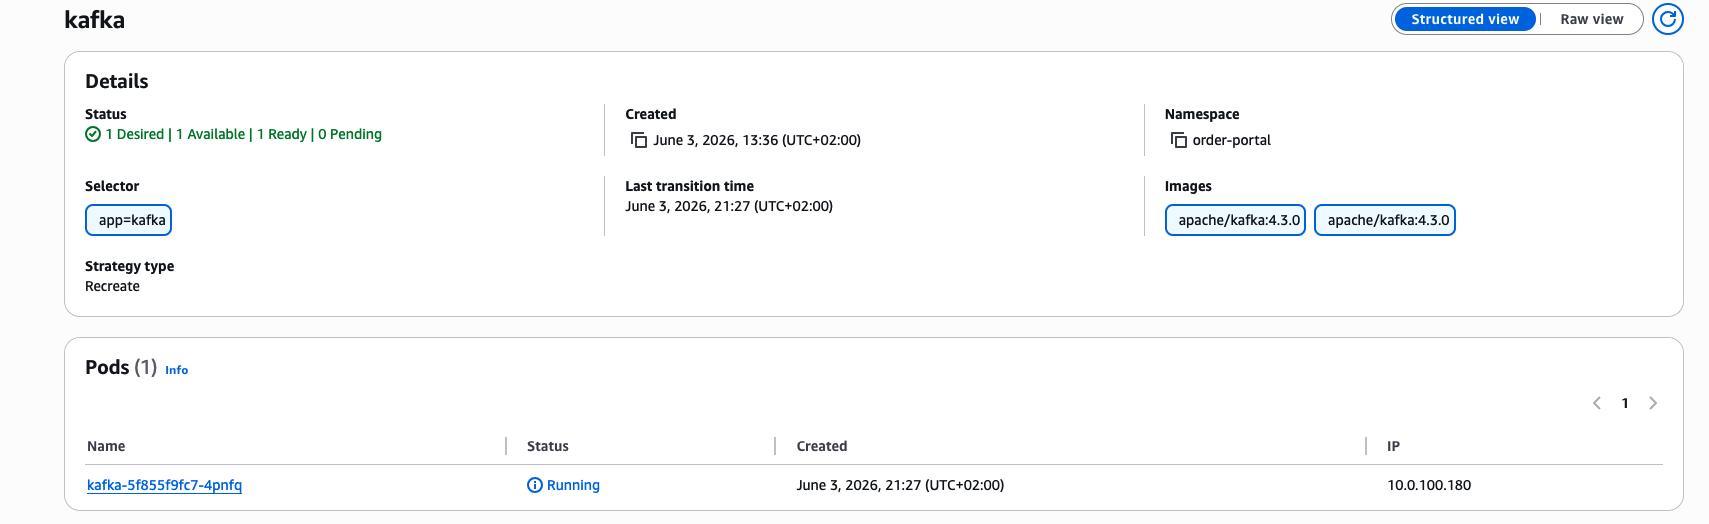
\includegraphics[width=\textwidth]{Kafka.png}
    \caption{Broker Apache Kafka (\code{apache/kafka:4.3.0}) uruchomiony w~klastrze jako pojedynczy pod, ze~strategią \emph{Recreate} --- zgodnie z~projektem jednowęzłowego brokera w~trybie KRaft.}
    \label{fig:kafka-eks}
\end{figure}

\section{Routing ruchu --- CloudFront, ALB i reverse proxy}
\label{sec:routing-ruchu}

Jedynym publicznym punktem wejścia do systemu jest dystrybucja CloudFront z~dwoma originami. Domyślne zachowanie
kieruje żądania do prywatnego bucketa S3 z~aplikacją webową, z~polityką agresywnego buforowania i~kompresją. Ponieważ trasy SPA (np.
\code{/orders/123}) nie odpowiadają obiektom w~S3, do zachowania dołączono funkcję CloudFront wykonywaną przy
każdym żądaniu (listing~\ref{lst:spa-router}). Żądania bez rozszerzenia pliku przepisywane są na \code{/index.html}, 
dzięki czemu głębokie odnośniki i~odświeżenie strony działają poprawnie.

\begin{lstlisting}[caption={Funkcja CloudFront przepisująca trasy SPA (cloudfront.tf)},label={lst:spa-router}]
function handler(event) {
  var request = event.request;
  var uri = request.uri;
  // No file extension (i.e. an app route, not an asset) -> serve the SPA.
  if (uri === "/" || uri.indexOf(".") === -1) {
    request.uri = "/index.html";
  }
  return request;
}
\end{lstlisting}

\begin{figure}[H]
    \centering
    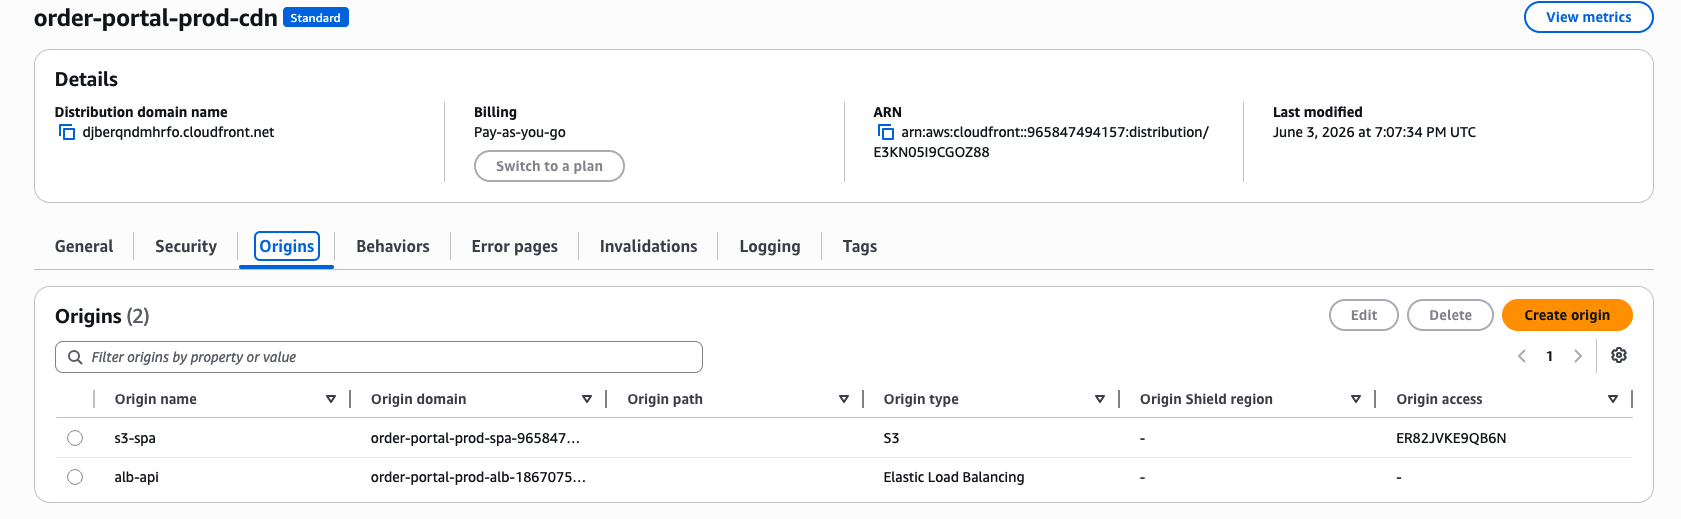
\includegraphics[width=\textwidth]{Cloudfront.png}
    \caption{Dystrybucja CloudFront \code{order-portal-prod-cdn} z~dwoma originami: bucketem S3 (aplikacja SPA, dostęp przez~Origin Access Control) oraz~load balancerem ALB (ruch API).}
    \label{fig:cloudfront}
\end{figure}

Żądania pasujące do wzorców \code{/api/*} oraz \code{/grafana*} obsługuje drugi origin Application Load
Balancer. Dostępu do samego ALB strzegą dwa niezależne mechanizmy. Po pierwsze, grupa bezpieczeństwa balancera dopuszcza ruch wyłącznie
z~zarządzanej listy prefiksów adresowych infrastruktury brzegowej CloudFront. Żądania spoza sieci CloudFront
nie nawiążą nawet połączenia TCP. Po drugie, CloudFront dokleja do żądań kierowanych do ALB tajny nagłówek
\code{X-Origin-Verify} (o~wartości generowanej zasobem \code{random\_password}), a~jedyna przepuszczająca reguła
nasłuchu wymaga jego obecności (listing~\ref{lst:origin-verify}). Żądania bez poprawnego nagłówka np.
z~cudzej dystrybucji CloudFront otrzymują odpowiedź odmowną. Wymusza to przepływ całego ruchu przez warstwę
brzegową, wraz z~jej terminacją TLS i~ochroną przed atakami wolumetrycznymi.

\begin{figure}[H]
    \centering
    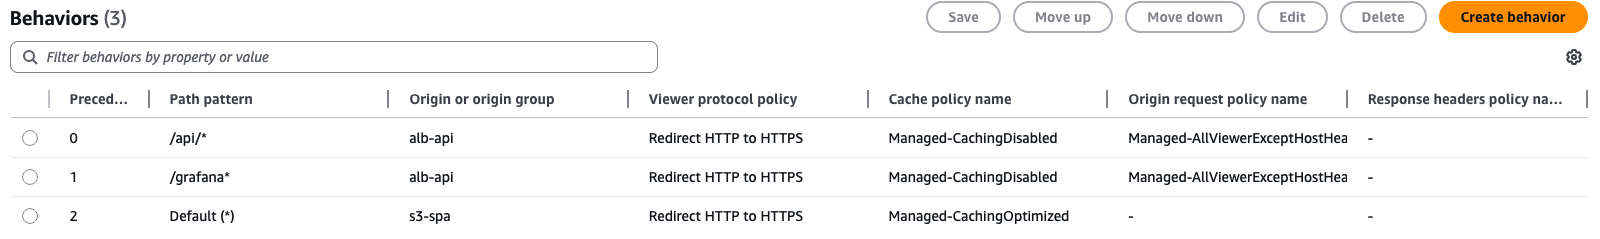
\includegraphics[width=\textwidth]{CloudfrontPaths.png}
    \caption{Reguły zachowań (\emph{behaviors}) CloudFront: ścieżki \code{/api/*} oraz~\code{/grafana*} kierowane są~do~ALB z~wyłączonym buforowaniem, a~pozostałe --- domyślnie do~bucketa S3 z~buforowaniem zoptymalizowanym.}
    \label{fig:cloudfront-paths}
\end{figure}

\begin{lstlisting}[caption={Reguła ALB wymagająca nagłówka weryfikacyjnego (alb.tf)},label={lst:origin-verify}]
resource "aws_lb_listener_rule" "from_cloudfront" {
  listener_arn = aws_lb_listener.http.arn
  priority     = 10

  condition {
    http_header {
      http_header_name = "X-Origin-Verify"
      values           = [random_password.origin_secret.result]
    }
  }

  action {
    type             = "forward"
    target_group_arn = aws_lb_target_group.app.arn
  }
}
\end{lstlisting}

Celem ALB jest grupa docelowa obejmująca węzły klastra
na porcie \code{NodePort} 30080, pod którym działa wewnętrzne odwrócone proxy. Proxy rozdziela ruch
na podstawie prefiksu ścieżki do usług klastra (listing~\ref{lst:nginx-routing}). Odpowiada na ścieżce
\code{/healthz} na potrzeby kontroli zdrowia ALB. Udostępnia również pod ścieżką \code{/grafana} interfejs
Grafany. Żądania niepasujące do żadnej reguły odrzuca. Pełna droga żądania API przebiega więc: przeglądarka
$\rightarrow$ CloudFront $\rightarrow$ ALB $\rightarrow$ NodePort $\rightarrow$ Proxy $\rightarrow$ Service
$\rightarrow$ pod mikroserwisu, co~ilustruje rysunek~\ref{fig:przeplyw-zadania}.

\begin{lstlisting}[caption={Reguły routingu wewnętrznego proxy nginx (fragment)},label={lst:nginx-routing}]
location = /healthz {
  add_header Content-Type text/plain;
  return 200 'ok';
}

location /api/v1/payments { proxy_pass http://payment-service:9003; }
location /api/orders      { proxy_pass http://order-service:9002; }
location /api/products    { proxy_pass http://product-service:9001; }

location / {
  add_header Content-Type text/plain;
  return 404 'not found';
}
\end{lstlisting}

\begin{figure}[H]
    \centering
    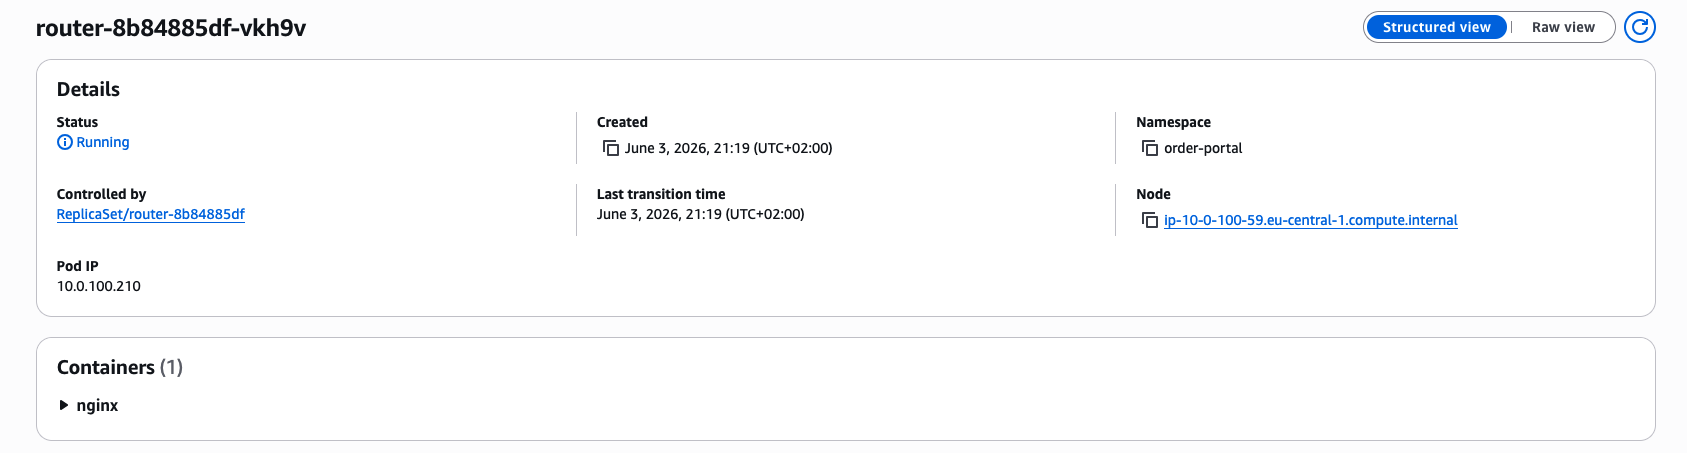
\includegraphics[width=\textwidth]{Nginx.png}
    \caption{Pod wewnętrznego proxy nginx (Deployment \code{router}) w~przestrzeni \code{order-portal} --- pojedyncza replika trasująca ruch API do~mikroserwisów na~podstawie prefiksu ścieżki.}
    \label{fig:nginx}
\end{figure}

\begin{figure}[H]
    \centering
    \begin{tikzpicture}[
        font=\scriptsize,
        >={Stealth[length=2.2mm]},
        layer/.style={
            rectangle,
            rounded corners=3pt,
            draw=black!45,
            thick,
            align=center,
            minimum height=11mm,
            minimum width=22mm,
            fill=#1
        },
        note/.style={
            align=center,
            font=\scriptsize,
            text=black!65
        },
        flow/.style={->, thick, draw=black!75},
        altflow/.style={->, thick, densely dashed, draw=black!60},
        lab/.style={
            midway,
            above,
            font=\scriptsize,
            fill=white,
            inner sep=1.5pt,
            align=center
        },
        node distance=11mm and 13mm
    ]

        % Main path
        \node[layer=blue!7] (br) {Przeglądarka};
        \node[layer=orange!10, right=of br] (cf) {CloudFront};
        \node[layer=green!9, right=of cf] (alb) {ALB};
        \node[layer=purple!8, right=of alb] (ng) {nginx\\NodePort};
        \node[layer=gray!10, right=of ng] (svc) {Mikroserwis};

        % API arrows
        \draw[flow] (br) -- node[lab] {HTTPS} (cf);
        \draw[flow] (cf) -- node[lab] {\texttt{/api/*}\\+ nagłówek} (alb);
        \draw[flow] (alb) -- node[lab] {\texttt{:30080}} (ng);
        \draw[flow] (ng) -- node[lab] {prefiks\\ścieżki} (svc);

        % SPA / S3 branch
        \node[layer=yellow!13, below=16mm of cf] (s3)
            {S3\\SPA};

        \draw[altflow] (cf) -- node[right, font=\scriptsize, fill=white, inner sep=1.5pt, align=center]
            {pozostałe\\trasy} (s3);

        % Security note
        \node[note, below=9mm of alb] (sec)
            {\textit{Ochrona dostępu do ALB}\\
             \texttt{X-Origin-Verify} + prefix list CloudFront};

        \draw[altflow] (sec.north) -- (alb.south);

        % Optional grouping labels
        \node[above=4mm of br, font=\scriptsize\bfseries, text=black!65]
            {Klient};

        \node[above=4mm of cf, font=\scriptsize\bfseries, text=black!65]
            {Edge};

        \node[above=4mm of alb, font=\scriptsize\bfseries, text=black!65]
            {Wejście do klastra};

        \node[above=4mm of ng, font=\scriptsize\bfseries, text=black!65]
            {Routing wewnętrzny};

        \node[above=4mm of svc, font=\scriptsize\bfseries, text=black!65]
            {Aplikacja};

    \end{tikzpicture}

    \caption{Przepływ żądania API przez warstwy systemu. CloudFront kieruje ruch \code{/api/*} do load balancera, natomiast pozostałe trasy obsługuje bucket S3 z aplikacją SPA. Dostęp do ALB ograniczają tajny nagłówek \code{X-Origin-Verify} oraz prefix list CloudFront. Wewnętrzne proxy nginx trasuje żądanie do właściwego mikroserwisu na podstawie prefiksu ścieżki.}
    \label{fig:przeplyw-zadania}
\end{figure}

\section{Wdrożenie monitoringu --- Prometheus i Grafana}
\label{sec:wdrozenie-monitoringu}

Podsystem monitoringu działa w~osobnej przestrzeni nazw \code{monitoring}. Serwer Prometheus skonfigurowano
z~15-sekundowym interwałem pomiarowym i~dynamicznym odkrywaniem celów poprzez API Kubernetes.
Reguły przeetykietowania (listing~\ref{lst:prometheus-scrape}) pozostawiają wyłącznie pody,
które jawnie zgłosiły się adnotacją \code{prometheus.io/scrape}. Czyli kierują pomiar na port i~ścieżkę wskazane
adnotacjami oraz wzbogacają metryki o~etykiety przestrzeni nazw i~poda. Objęcie monitoringiem nowej usługi nie
wymaga więc żadnych zmian po stronie Prometheusa. Wystarczą adnotacje w~jej szablonie poda. Uprawnienia do
odczytu metadanych podów nadano dedykowanemu kontu usługi poprzez rolę klastrową RBAC, a~baza szeregów czasowych
składowana jest na trwałym woluminie \code{ebs-gp3} o~pojemności 5~GiB.

\begin{lstlisting}[caption={Odkrywanie celów pomiarowych na podstawie adnotacji (prometheus.yml)},label={lst:prometheus-scrape}]
scrape_configs:
  - job_name: kubernetes-pods
    kubernetes_sd_configs:
      - role: pod
    relabel_configs:
      - source_labels: [__meta_kubernetes_pod_annotation_prometheus_io_scrape]
        action: keep
        regex: "true"
      - source_labels: [__meta_kubernetes_pod_annotation_prometheus_io_path]
        action: replace
        target_label: __metrics_path__
        regex: (.+)
      - source_labels: [__address__, __meta_kubernetes_pod_annotation_prometheus_io_port]
        action: replace
        regex: ([^:]+)(?::\d+)?;(\d+)
        replacement: $1:$2
        target_label: __address__
\end{lstlisting}

Grafanę provisionowano w~pełni deklaratywnie: źródło danych (wewnątrzklastrowy adres Prometheusa).
 Interfejs Grafany udostępniono pod ścieżką \code{/grafana} publicznej dystrybucji CloudFront (poprzez regułę proxy z~sekcji~\ref{sec:routing-ruchu}), dzięki
czemu wgląd w~stan systemu nie wymaga dostępu administracyjnego do klastra.

\begin{figure}[H]
    \centering
    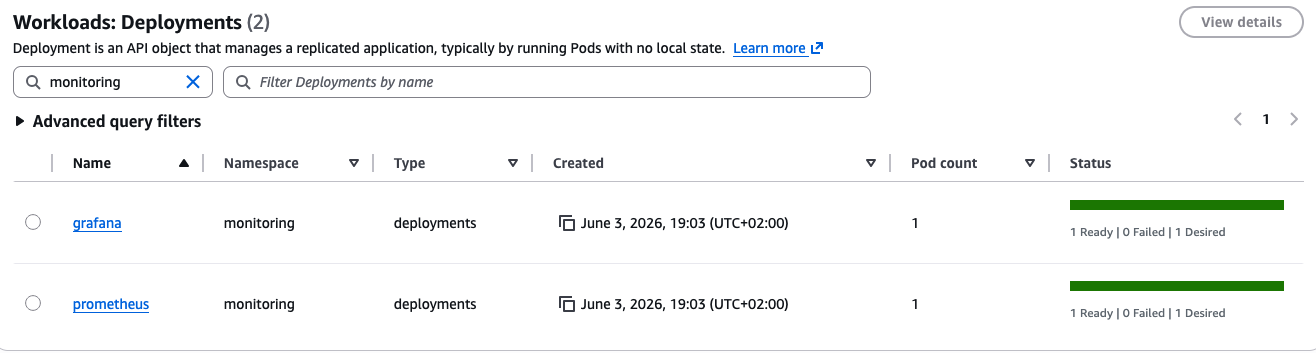
\includegraphics[width=\textwidth]{PrometheusEKS.png}
    \caption{Podsystem monitoringu w~przestrzeni nazw \code{monitoring}: wdrożenia Prometheus i~Grafana, oba w~stanie gotowości.}
    \label{fig:prometheus-eks}
\end{figure}

\begin{figure}[H]
    \centering
    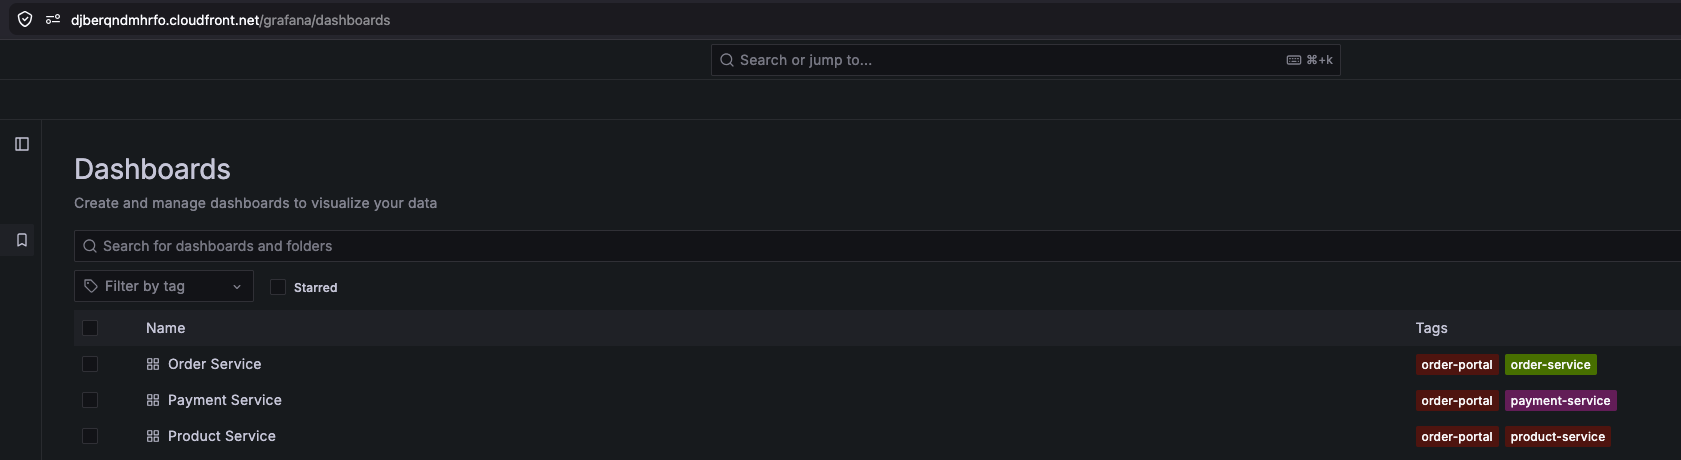
\includegraphics[width=\textwidth]{Grafana.png}
    \caption{Interfejs Grafany udostępniony pod~ścieżką \code{/grafana} dystrybucji CloudFront, z~osobnym kokpitem dla~każdego z~trzech mikroserwisów.}
    \label{fig:grafana}
\end{figure}

\section{Skalowanie aplikacji i zarządzanie cyklem życia}
\label{sec:skalowanie-i-cykl-zycia}

Skalowanie poziome zdefiniowano obiektami HorizontalPodAutoscaler dla serwisów zamówień i~produktów. Usług
przyjmujących główny ruch systemu. Liczba replik zmienia się w~przedziale od~1 do~2 tak, aby średnie wykorzystanie
procesora utrzymywało się poniżej progu zadanego jako odsetek wartości żądanej (\emph{request}). Próg ten jest
parametrem infrastruktury (zmienna \code{hpa\_cpu\_target}). Wartość początkową 80\% obniżono do 60\% na
podstawie testów obciążeniowych. Przy wyższym progu skalowanie nie wyzwalało się przed nasyceniem węzłów.
Niższy próg pozwala dołożyć replikę z~wyprzedzeniem, zanim rosnący ruch wyczerpie zapas mocy
(proces strojenia opisano w~rozdziale~\ref{chap:testy-i-analiza}). Źródłem metryk dla HPA jest komponent
\code{metrics-server}, który nie wchodzi w~skład domyślnej instalacji EKS. Zainstalowano go jako zarządzany dodatek EKS (\emph{community add-on}) zasobem
\code{aws\_eks\_addon}, analogicznie do pozostałych dodatków klastra. Wąski przedział replik jest konsekwencją pojemności
środowiska. Czterowęzłowy klaster instancji \code{t3.small} mieści ograniczoną liczbę podów. Zachowanie HPA pod
obciążeniem zbadano w~rozdziale~\ref{chap:testy-i-analiza}.

Cykl życia aplikacji zarządzany jest przez zmiany w~kodzie infrastruktury. Nowa wersja obrazu wskazywana jest
zmienną \code{image\_tag}, a~\code{terraform apply} aktualizuje Deploymenty.
\chapter{Testy i analiza działania systemu}
\label{chap:testy-i-analiza}

Rozdział przedstawia weryfikację systemu wdrożonego w~docelowym środowisku chmurowym. Omówiono metodykę
testowania, wyniki testów funkcjonalnych oraz testy wydajnościowe i~skalowalności. Rozdział zamykają: analiza kosztów
utrzymania środowiska oraz identyfikacja wąskich gardeł wraz z~rekomendacjami optymalizacji.

\section{Metodyka testowania}
\label{sec:metodyka-testowania}

Testy wydajnościowe zrealizowano narzędziem \textbf{k6}, generującym ruch HTTP według programowalnych scenariuszy.
Obciążenie kierowano na \emph{publiczny} punkt wejścia systemu - dystrybucję CloudFront. Dzięki czemu pomiar
obejmuje całą produkcyjną ścieżkę żądania (sekcja~\ref{sec:routing-ruchu}). Zdefiniowano dwa współbieżne scenariusze odzwierciedlające
realny ruch. \emph{Przeglądanie} czyli listowanie i~filtrowanie katalogu, przegląd zamówień co stanowi większość żądań. 
\emph{Zakup} czyli złożenie zamówienia, oczekiwanie na asynchroniczną walidację, utworzenie i~finalizacja płatności. 
Liczbę wirtualnych użytkowników (VU) zwiększano etapowo według czterech profili zestawionych w~tabeli~\ref{tab:profile-testowe}.

\begin{table}[H]
    \centering
    \caption{Profile testów wydajnościowych}
    \label{tab:profile-testowe}
    \begin{tabular}{lllp{6.2cm}}
        \toprule
        \textbf{Profil} & \textbf{Maks. VU} & \textbf{Czas} & \textbf{Cel} \\
        \midrule
        load   & 25  & 8 min  & zachowanie przy ruchu nominalnym \\
        stress & 115 & 10 min & poszukiwanie granicy wydajności \\
        max    & 280 & 10 min & wymuszenie automatycznego skalowania \\
        \bottomrule
    \end{tabular}
\end{table}

Kluczową metryką własną jest \emph{opóźnienie walidacji zamówienia}. Jest to czas od~utworzenia zamówienia do
osiągnięcia przez nią statusu \code{VALIDATED}, mierzony przez cykliczne odpytywanie (co~500~ms). Obejmuje on całą
ścieżkę asynchronicznej choreografii. Publikację zdarzenia do Kafki, jego konsumpcję przez product-service,
rezerwację stanów magazynowych i~zapis statusu. Należy zaznaczyć, że rozdzielczość tego pomiaru ograniczona jest
interwałem odpytywania, co omówiono przy interpretacji wyników. Stan systemu w~trakcie testów obserwowano
w~Grafanie (metryki techniczne i~domenowe z~Prometheusa) oraz poleceniami \code{kubectl} (stan
HorizontalPodAutoscaler oraz zużycie zasobów podów). Profile procesora pobierano przez \code{pprof}
(sekcja~\ref{subsec:profilowanie}). Katalog zasiano produktami o~wysokim stanie magazynowym, aby rezerwacje nie
wyczerpały zapasów w~trakcie testu.

\section{Testy funkcjonalne systemu}
\label{sec:testy-funkcjonalne}

Poprawność funkcjonalną zweryfikowano scenariuszami pokrywającymi główne przypadki użycia, wykonanymi zarówno
manualnie przez portal, jak i masowo jako część scenariusza zakupowego testów wydajnościowych. Wyniki
przedstawiono w tabeli~\ref{tab:testy-funkcjonalne}.

\begin{table}[H]
    \centering
    \caption{Scenariusze testów funkcjonalnych}
    \label{tab:testy-funkcjonalne}
    \begin{tabular}{p{7.2cm}p{4.5cm}c}
        \toprule
        \textbf{Scenariusz} & \textbf{Oczekiwany wynik} & \textbf{Rezultat} \\
        \midrule
        Logowanie przez Cognito (OAuth 2.0 + PKCE) & przekierowanie, wydanie tokenu & \checkmark \\
        Przeglądanie i~filtrowanie katalogu & lista zgodna z~filtrami & \checkmark \\
        Złożenie zamówienia & status \code{NEW}, zdarzenie \code{order.created} & \checkmark \\
        Automatyczna walidacja i~rezerwacja & przejście do \code{VALIDATED} & \checkmark \\
        Powtórzone żądanie z~tym samym kluczem & brak duplikatu zamówienia & \checkmark \\
        Zamówienie produktu bez stanu & odrzucenie rezerwacji, \code{CANCELLED} & \checkmark \\
        Pełna płatność za zamówienie & \code{PAID} / \code{SUCCEEDED} & \checkmark \\
        Dostęp do cudzego zamówienia & odmowa (autoryzacja po~tokenie) & \checkmark \\
        Próba opłacenia anulowanego zamówienia & odrzucenie (maszyna stanów) & \checkmark \\
        \bottomrule
    \end{tabular}
\end{table}

Szczególnie istotny jest masowy dowód poprawności płynący z~testów wydajnościowych. W~najcięższym profilu
\emph{max} system przyjął \textbf{7564 zamówienia}, z~których \textbf{wszystkie} przeszły pełny cykl od~utworzenia,
przez walidację, po~finalizację płatności. Bez ani jednego błędu HTTP, niespójności stanu czy nieudanej
rezerwacji. Potwierdza to poprawność maszyny stanów, mechanizmu idempotencji oraz transakcyjnej finalizacji
płatności w~warunkach wysokiej współbieżności.

\section{Testy wydajnościowe i skalowalność}
\label{sec:testy-wydajnosciowe}

Zbiorcze wyniki czterech profili przedstawia tabela~\ref{tab:wyniki-wydajnosc}. We~wszystkich przebiegach odsetek
błędnych odpowiedzi HTTP wyniósł \textbf{0\%}, a~wszystkie kryteria akceptacji (progi czasów odpowiedzi i~odsetka
błędów) zostały spełnione.ń

\begin{table}[H]
    \centering
    \caption{Wyniki testów wydajnościowych (czasy w ms)}
    \label{tab:wyniki-wydajnosc}
    \small
    \begin{tabular}{lrrrrrr}
        \toprule
        \textbf{Profil} & \textbf{Żądań} & \textbf{Przeł.\ [req/s]} & \textbf{HTTP p95} & \textbf{HTTP p99} & \textbf{Walid.\ med.} & \textbf{Zamówień} \\
        \midrule
        load   & 5\,462   & 11{,}2  & 600 & 1\,871 & 543 & 385 \\
        stress & 19\,921  & 32{,}9  & 118 & 757    & 542 & 981 \\
        max    & 267\,643 & 445{,}5 & 92  & 185    & 547 & 7\,564 \\
        \bottomrule
    \end{tabular}
\end{table}

\subsection{Czasy odpowiedzi i efekt rozgrzania}
\label{subsec:czasy-odpowiedzi}

Przy najwyższym obciążeniu (445~req/s, 280~VU) mediana czasu odpowiedzi API wyniosła~49~ms, a~95.~percentyl
92~ms. Są to wyniki bardzo dobre, zważywszy na minimalne zasoby środowiska (cztery instancje \code{t3.small}).

Uwagę zwraca kontrintuicyjna zależność. Czasy odpowiedzi \emph{malały} wraz ze~wzrostem obciążenia. Zjawisko to wynika
z~efektu rozgrzania. Profil \emph{load} był pierwszym przebiegiem po~wdrożeniu, wykonywanym na~,,zimnym''
systemie z~pustymi pulami połączeń do~bazy danych, nieuzupełnionym cache kluczy JWKS oraz niewykorzystanym
zapasem kredytów procesora instancji. Kolejne przebiegi korzystały już z~rozgrzanych zasobów.
Wniosek metodyczny to konieczność rozgrzania systemu przed pomiarem wydajności odnotowano jako istotny dla
wiarygodności tego typu testów.

\subsection{Opóźnienie asynchronicznej walidacji}
\label{subsec:opoznienie-walidacji}

Mediana opóźnienia walidacji zamówienia okazała się \emph{niewrażliwa} na~obciążenie. Wyniosła 543, 542 i~547~ms
odpowiednio w~profilach \emph{load}, \emph{stress} i~\emph{max}, mimo czterdziestokrotnego wzrostu przepustowości.
Oznacza to, że asynchroniczna ścieżka oparta na~Kafce nie stała się wąskim gardłem nawet przy~445~req/s.
Przetwarzanie zdarzeń nadążało za~ich napływem, bez narastania zaległości w~kolejce.

Wartość ta wymaga interpretacji w~świetle metodyki. Status zamówienia odpytywano co~500~ms, mediana
bliska~540~ms oznacza, że zamówienie było już zwalidowane przy~\emph{pierwszym} odpytaniu (po~ok.~500~ms snu),
a~rzeczywiste opóźnienie choreografii zdarzeń jest istotnie niższe niż~zmierzone. Pomiar jest skwantowany
rozdzielczością odpytywania. Wynik należy zatem traktować jako~\emph{górne ograniczenie} faktycznego opóźnienia,
które sądząc po~niewielkim rozrzucie wartości (95.~percentyl 590~ms w~profilu \emph{max}) mieści się
w~granicach pojedynczych dziesiątek do~setki milisekund.

\subsection{Automatyczne skalowanie pod obciążeniem}
\label{subsec:skalowanie-pod-obciazeniem}

Profil \emph{stress} (do~115~VU) system obsłużył bez~uruchomienia skalowania. Przy~progu HorizontalPodAutoscaler
ustawionym pierwotnie na~80\% wykorzystania procesora względem żądania, obciążenie poszczególnych podów nie
przekroczyło tej wartości, a~zużycie procesora węzłów sięgnęło~ok.~60\%. Obserwacja ta skłoniła do~obniżenia progu
HPA do~60\% (sekcja~\ref{sec:skalowanie-i-cykl-zycia}), aby skalowanie wyprzedzało nasycenie.

W~profilu \emph{max} mechanizm zadziałał zgodnie z~projektem. Wraz ze~wzrostem ruchu wykorzystanie procesora
serwisu produktów przekroczyło próg, co~wyzwoliło zwiększenie liczby replik z~jednej do~dwóch. Analogicznie
przeskalowany został serwis zamówień. Przebieg skalowania ilustruje fragment~\ref{lst:hpa-scaling} 
ciągłej obserwacji stanu HPA, na~którym widać przekroczenie progu i~następujące po~nim zwiększenie liczby
replik.

\begin{lstlisting}[caption={Reakcja HorizontalPodAutoscaler na obciążenie (profil max)},label={lst:hpa-scaling}]
NAME              REFERENCE                TARGETS        REPLICAS
product-service   .../product-service      cpu: 41%/60%   1
product-service   .../product-service      cpu: 79%/60%   1
product-service   .../product-service      cpu: 109%/60%  2   <- skalowanie
order-service     .../order-service         cpu: 65%/60%   1
order-service     .../order-service         cpu: 95%/60%   2   <- skalowanie
product-service   .../product-service      cpu: 264%/60%  2   <- limit replik
\end{lstlisting}

Po~osiągnięciu maksymalnej liczby replik (2, ograniczonej pojemnością czterech węzłów klastra) wykorzystanie
procesora pojedynczego poda produktów rosło dalej (do~ponad~260\% wartości żądanej). Co~unaocznia granicę
skalowania poziomego przy~stałej liczbie węzłów. Po~wyczerpaniu limitu replik dalszy wzrost ruchu absorbowany jest
już~tylko przez~rezerwę wydajności istniejących podów (limit~CPU ustawiono pięciokrotnie powyżej żądania)
Mimo to system pozostał w~pełni sprawny, bez~błędów i~przy~niskich czasach odpowiedzi. 
To~potwierdza, że nawet zsumowane obciążenie szczytowe mieściło się w~zapasie mocy obliczeniowej klastra.

Zachowanie systemu w~profilu \emph{max} ilustrują kokpity Grafany. Ilustracja~\ref{fig:grafana-order} przedstawia
metryki serwisu zamówień: charakterystyczne rozdwojenie wykresu zużycia procesora i~pamięci w~momencie pojawienia
się drugiej repliki, narastającą przepustowość żądań oraz tempo tworzenia zamówień. Ilustracja~\ref{fig:grafana-product}
prezentuje analogiczne metryki serwisu produktów wraz z~tempem konsumpcji zdarzeń z~Kafki.

\begin{figure}[H]
    \centering
    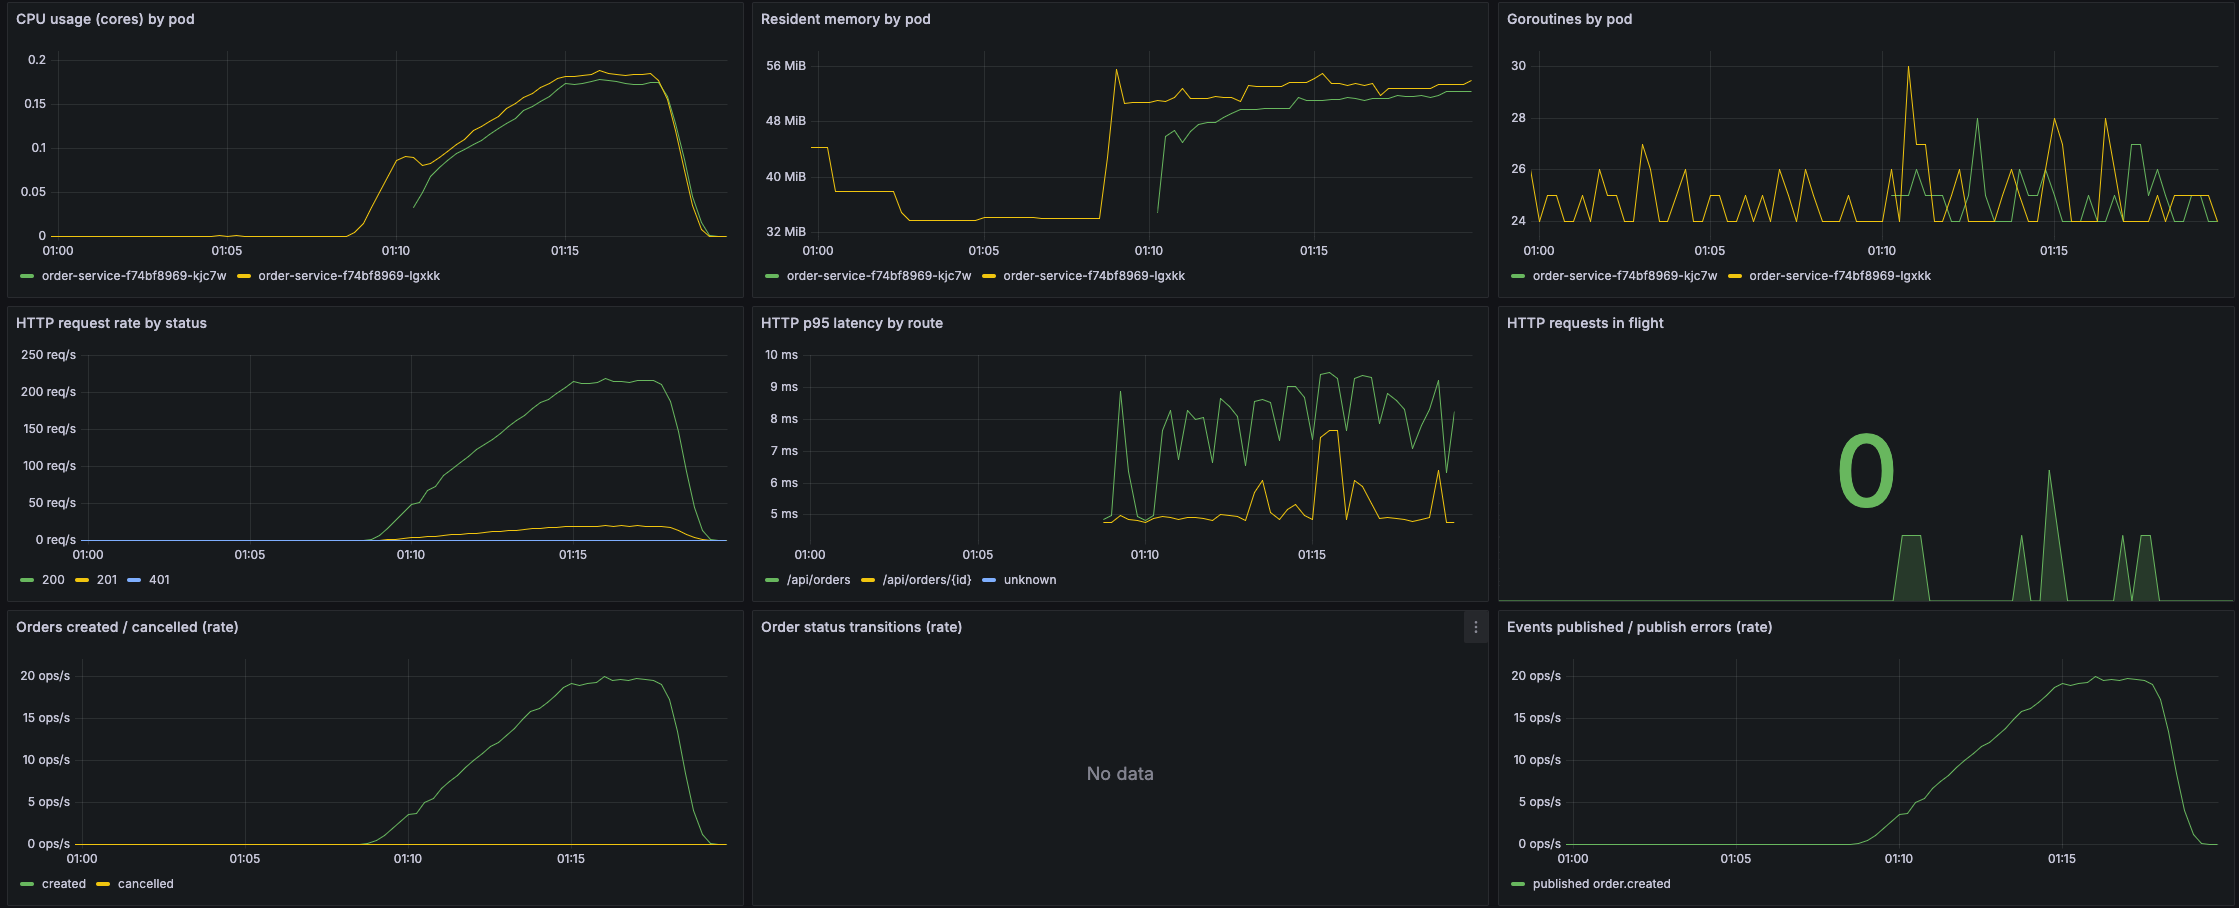
\includegraphics[width=\textwidth]{max-grafana-order.png}
    \caption{Metryki serwisu zamówień w~profilu \emph{max} (Grafana): zużycie procesora i~pamięci per replika, przepustowość HTTP, opóźnienia oraz tempo tworzenia zamówień. Rozdwojenie krzywych obrazuje moment automatycznego skalowania do~dwóch replik. (źródło: opracowanie własne)}
    \label{fig:grafana-order}
\end{figure}

\begin{figure}[H]
    \centering
    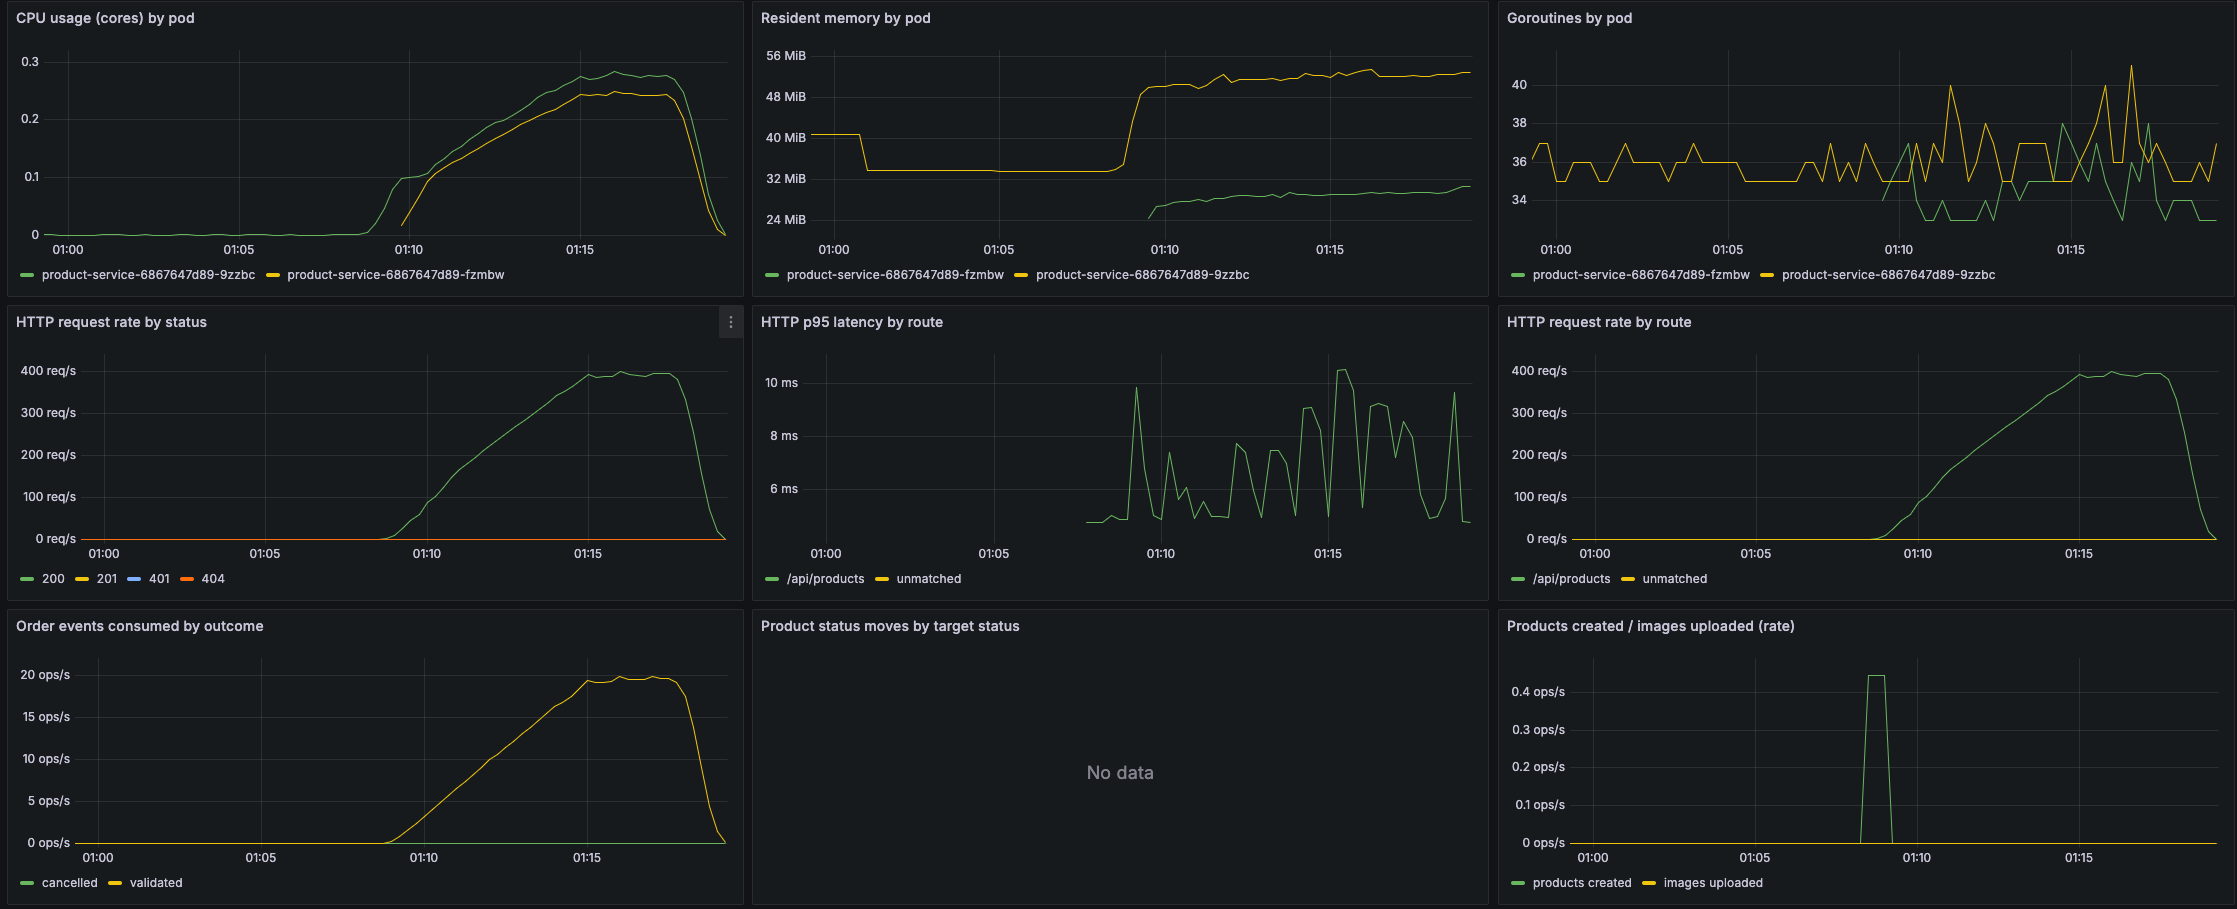
\includegraphics[width=\textwidth]{max-grafana-product.png}
    \caption{Metryki serwisu produktów w~profilu \emph{max} (Grafana): zużycie zasobów per replika, przepustowość oraz tempo konsumpcji zdarzeń z~Kafki. (źródło: opracowanie własne)}
    \label{fig:grafana-product}
\end{figure}

\section{Analiza kosztowa wykorzystania usług AWS}
\label{sec:analiza-kosztowa}

Rzeczywiste koszty utrzymania środowiska, odczytane z~usługi AWS Cost Explorer, przedstawiają
rysunki~\ref{fig:june-billing} i~\ref{fig:forecast-cost}.

\begin{figure}[H]
    \centering
    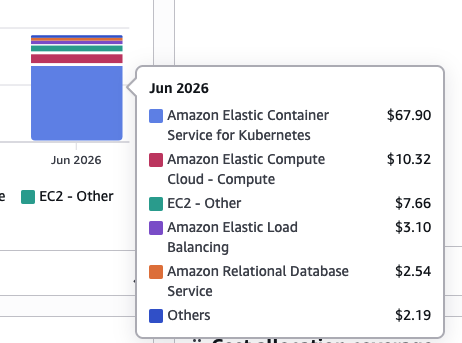
\includegraphics[scale=0.6]{JuneBilling.png}
    \caption{Rzeczywisty koszt środowiska w~czerwcu 2026 w~podziale na~usługi (AWS Cost Explorer). Dominuje płaszczyzna sterowania EKS (67,90~USD) - składnik nieobjęty bezpłatnym limitem; pozostałe usługi (EC2, ELB, RDS) generują koszty rzędu pojedynczych dolarów dzięki Free Tier. (źródło: opracowanie własne)}
    \label{fig:june-billing}
\end{figure}

\begin{figure}[H]
    \centering
    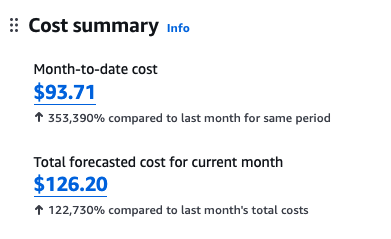
\includegraphics[scale=0.6]{ForecastCost.png}
    \caption{Podsumowanie kosztów bieżącego miesiąca (AWS Cost Explorer): koszt narosły do~dnia odczytu (93,71~USD) oraz~prognoza na~cały miesiąc (126,20~USD). (źródło: opracowanie własne)}
    \label{fig:forecast-cost}
\end{figure}

\subsection{Profilowanie procesora}
\label{subsec:profilowanie}

Profile procesora serwisów, pobrane przez~\code{pprof} w~szczycie obciążenia profilu \emph{max}, wskazują, że~obie
usługi są~\emph{ograniczone operacjami wejścia-wyjścia}, nie~zaś mocą obliczeniową. Dominującą pozycją w~obu
profilach są~wywołania systemowe (ok.~18\% próbek dla~serwisu zamówień, ok.~22\% dla~produktów) związane
z~komunikacją sieciową oraz~zapytaniami do~bazy danych. Całkowite zużycie procesora w~oknie pomiaru pozostawało
niskie. Oznacza to, że~kod aplikacyjny w~języku~Go nie~jest czynnikiem ograniczającym wydajność. Profile obu
serwisów w~postaci wykresów płomieniowych (\emph{flamegraph}) przedstawiono na~rysunkach~\ref{fig:order-service-flamegraph}
i~\ref{fig:product-service-flamegraph}.

\begin{figure}[H]
    \centering
    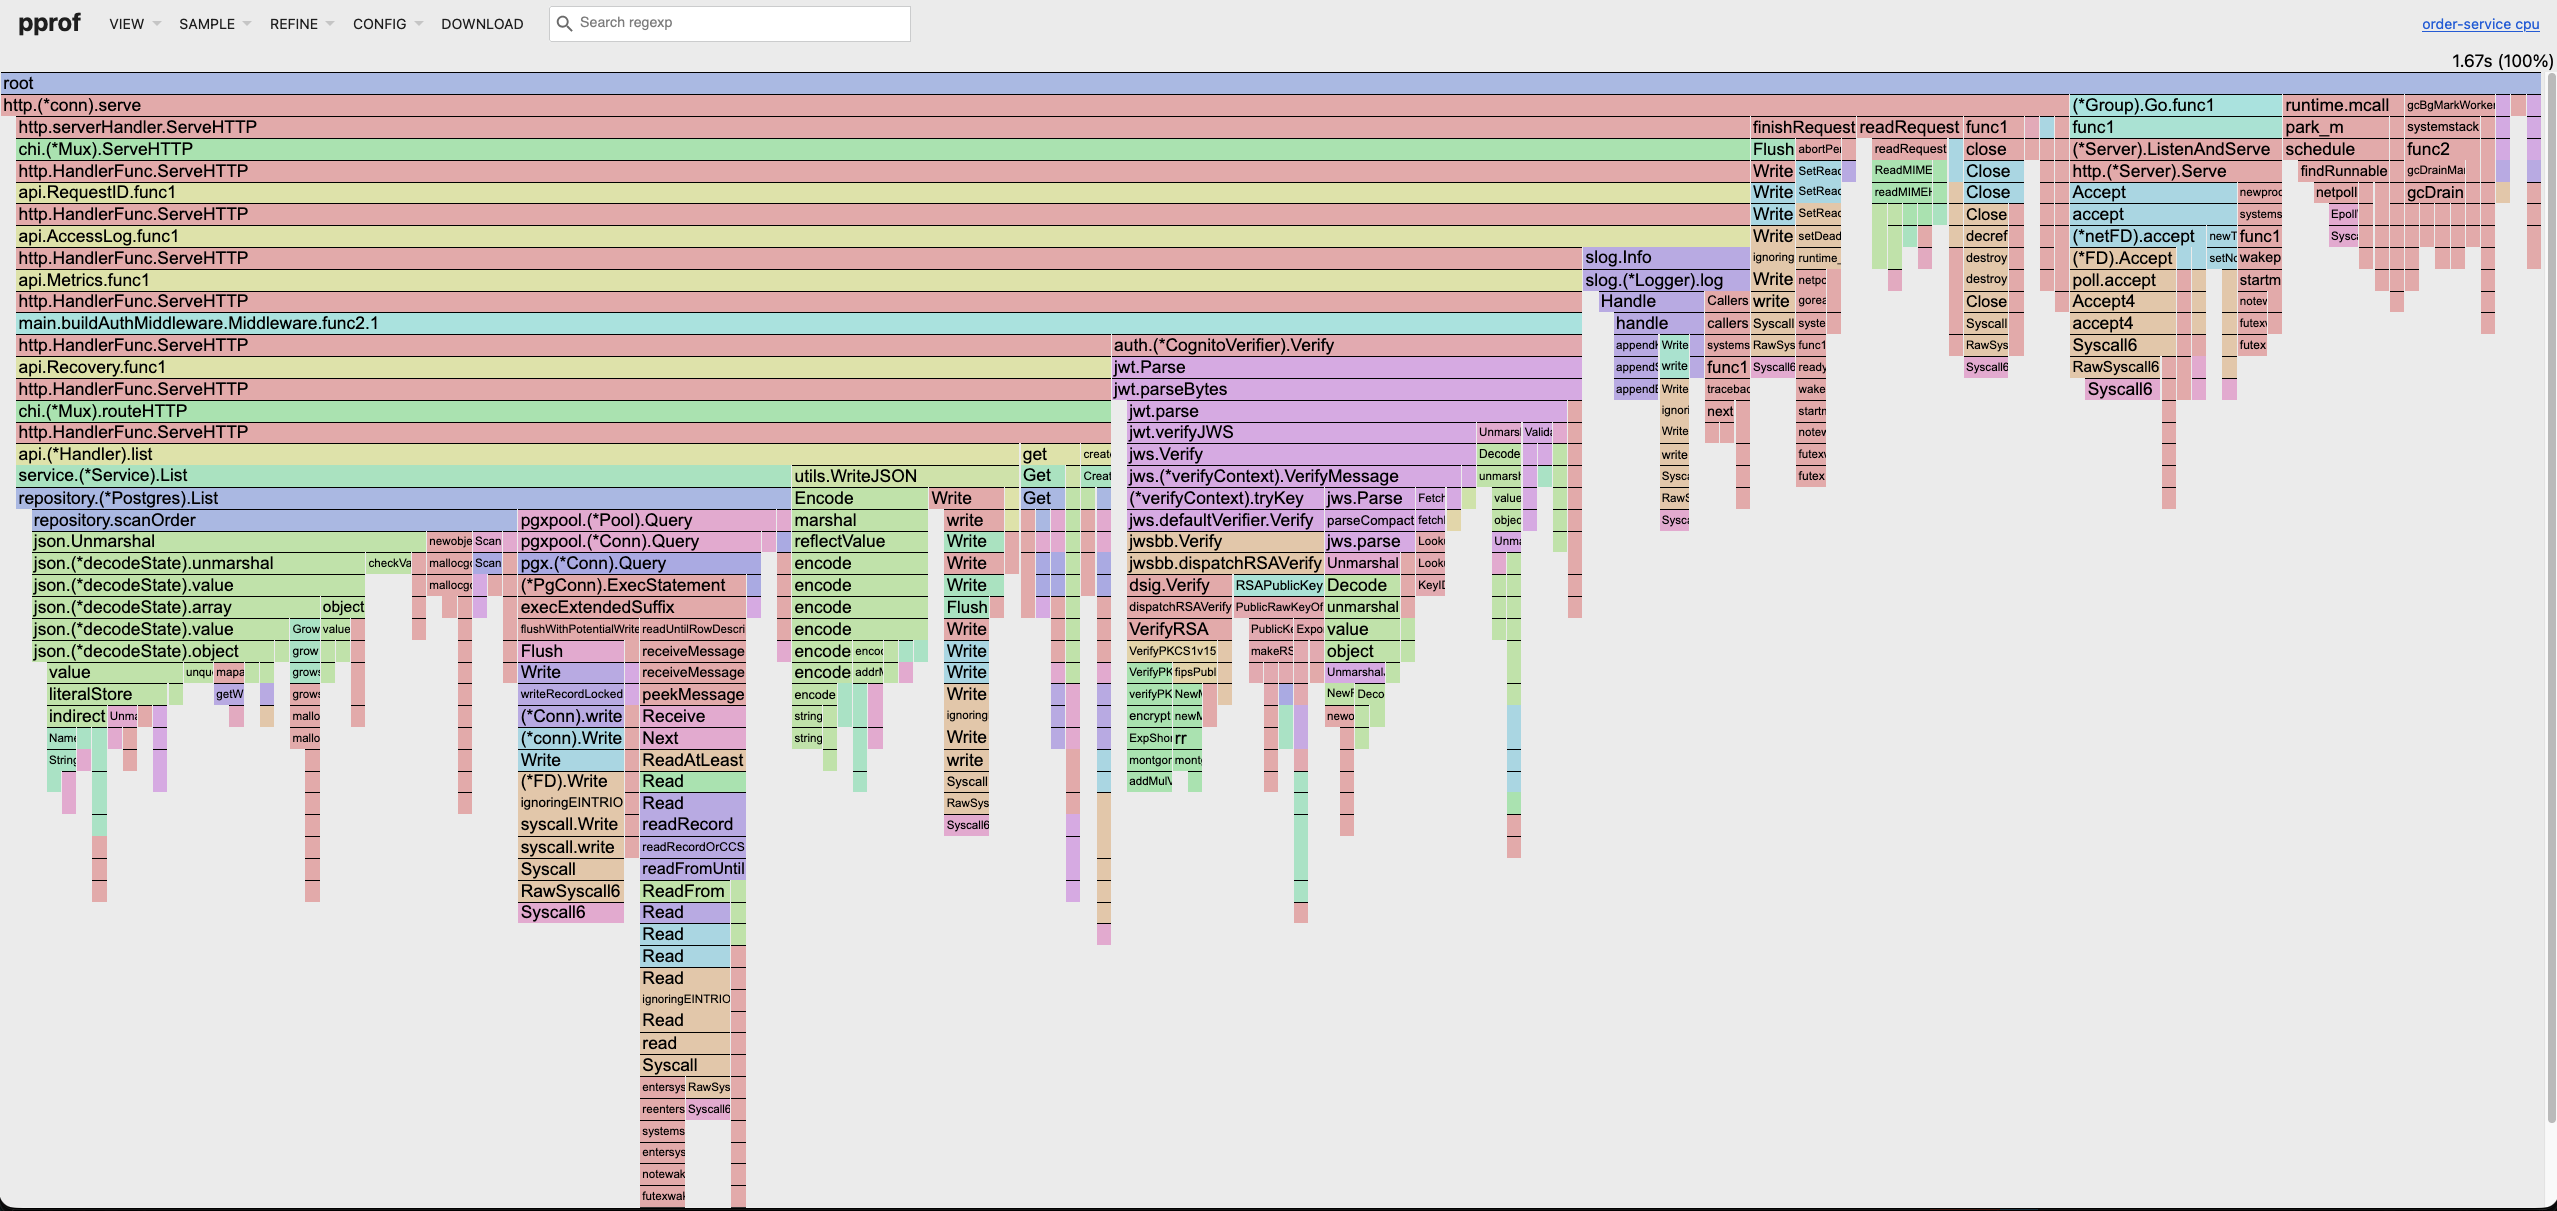
\includegraphics[width=\textwidth]{order-service-flamegraph.png}
    \caption{Flamegraph profilu procesora serwisu zamówień (\code{pprof}), zarejestrowany w~szczycie obciążenia profilu \emph{max}. Szerokość słupka odpowiada udziałowi funkcji w~czasie procesora. Widoczne są: obsługa żądań HTTP, weryfikacja tokenu JWT (\code{CognitoVerifier.Verify}), zapytania do~PostgreSQL przez~\code{pgx} oraz~(de)serializacja JSON. Znaczną część stanowią wywołania systemowe związane z~siecią i~bazą danych, co~potwierdza ograniczenie operacjami wejścia-wyjścia, nie~mocą obliczeniową. (źródło: opracowanie własne)}
    \label{fig:order-service-flamegraph}
\end{figure}

\begin{figure}[H]
    \centering
    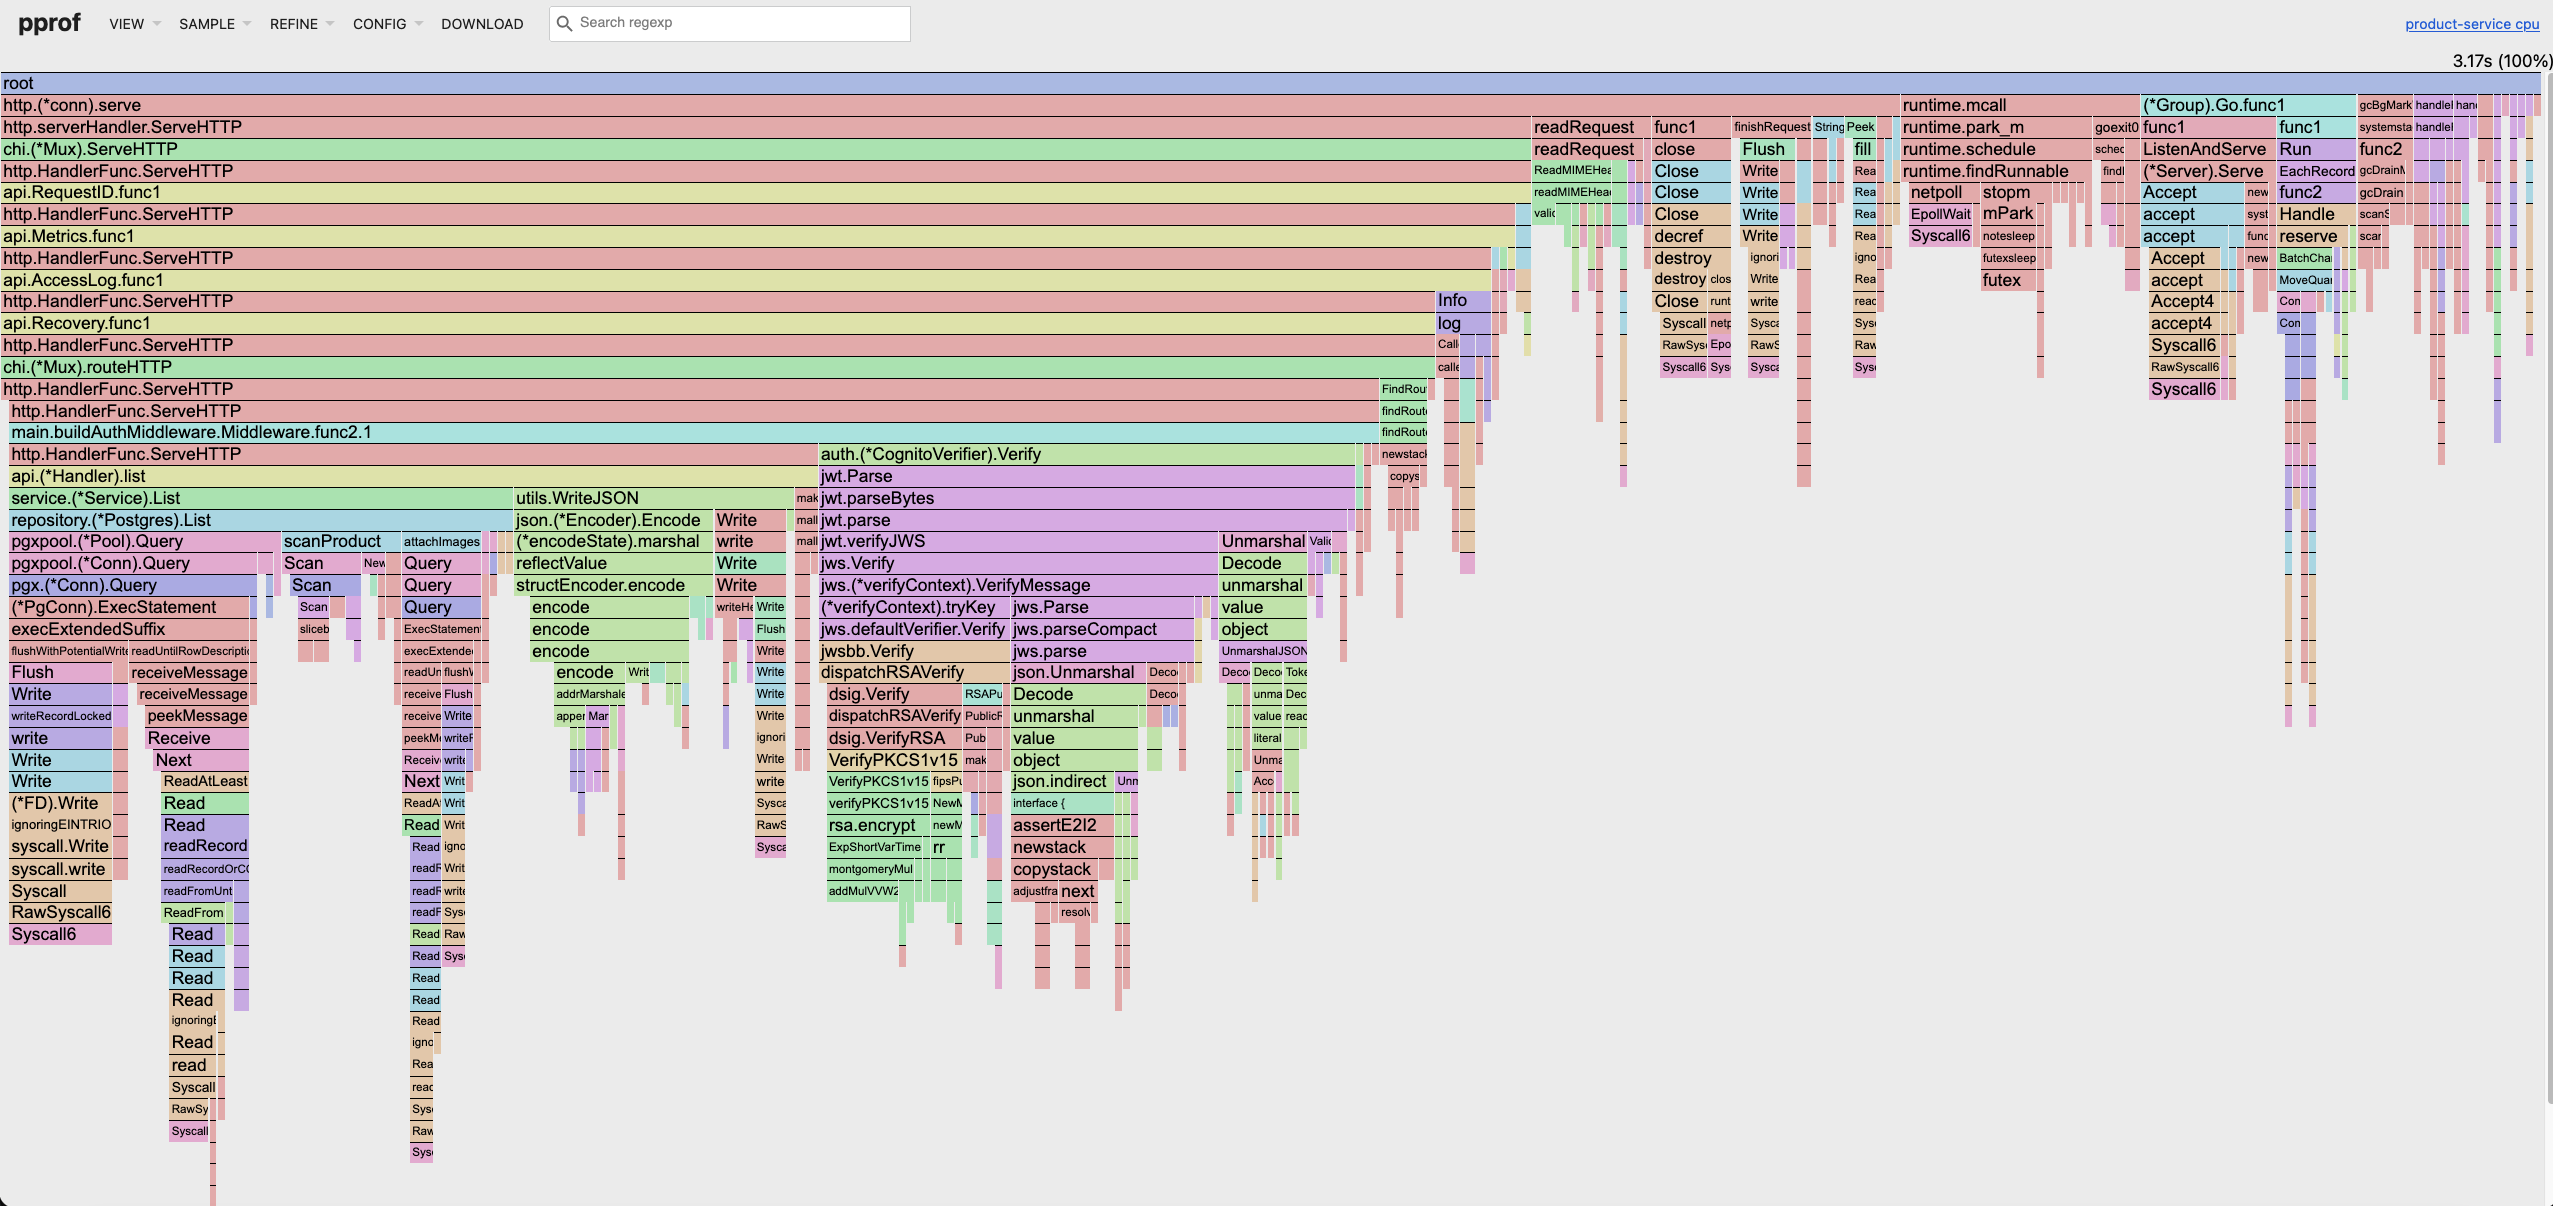
\includegraphics[width=\textwidth]{product-service-flamegraph.png}
    \caption{Flamegraph profilu procesora serwisu produktów (\code{pprof}) w~szczycie obciążenia profilu \emph{max}. Podobnie jak w~serwisie zamówień dominują wywołania systemowe (operacje sieciowe i~bazodanowe), a~spośród operacji obliczeniowych wyróżniają się weryfikacja JWT oraz~kodowanie JSON - profil potwierdza, że~usługa jest~ograniczona wejściem-wyjściem. (źródło: opracowanie własne)}
    \label{fig:product-service-flamegraph}
\end{figure}

Spośród operacji czysto obliczeniowych w~profilach wyróżniają się dwie. Pierwszą jest~weryfikacja podpisu tokenu
JWT (operacje arytmetyki wielokrotnej precyzji klucza~RSA, widoczne w~obu serwisach). Powtarzana przy~każdym
żądaniu, mimo że~ten~sam token powtarza się w~wielu kolejnych żądaniach tego~samego użytkownika. Drugą jest
serializacja i~deserializacja JSON (ok.~8\% próbek w~serwisie produktów). Obie wskazują konkretne kierunki
optymalizacji, gdyby~system stał się ograniczony procesorem. Buforowanie wyniku weryfikacji tokenu na~czas jego
ważności oraz ewentualna zamiana refleksyjnego kodowania JSON na~generowany statycznie.

\subsection{Zidentyfikowane wąskie gardła}
\label{subsec:waskie-gardla-lista}

Analiza zachowania systemu pod~obciążeniem oraz~jego architektury pozwala wskazać następujące ograniczenia
i~rekomendacje:

\begin{itemize}
    \item \textbf{Pamięć węzłów, nie~procesor.} W~spoczynku węzły wykorzystują~53-76\% pamięci przy~znikomym
    zużyciu procesora; głównym konsumentem pamięci jest broker Kafka (ok.~570~MiB), podczas gdy~mikroserwisy~Go
    zużywają zaledwie~po~10-35~MiB. Na~instancjach \code{t3.small} (2~GiB) to~pamięć, a~nie~procesor, ogranicza
    gęstość podów. Co~oznacza, że~skalowane przez~HPA według~procesora repliki mogą~w~skrajnym przypadku
    nie~znaleźć węzła z~wolną pamięcią.

    \item \textbf{Wewnętrzne proxy jako pojedynczy punkt.} Pod~nginx pełniący rolę reverse proxy
    (sekcja~\ref{sec:routing-ruchu}) działa w~jednej replice i~w~szczycie obciążenia zużywał~ok.~220~m~CPU.
    Porównywalnie z~pojedynczą repliką mikroserwisu. Stanowi on~zarówno pojedynczy punkt awarii, jak~i~potencjalne
    wąskie gardło. Rekomendacją jest~jego replikacja i~objęcie automatycznym skalowaniem.

    \item \textbf{Pojedynczy broker Kafka.} Broker działa w~jednej replice z~woluminem o~dostępie wyłącznym
    (sekcja~\ref{sec:wdrozenie-do-klastra}). Jego awaria wstrzymuje całą asynchroniczną walidację zamówień.
    W~środowisku produkcyjnym wymagałby klastra lub~usługi zarządzanej (Amazon~MSK).

    \item \textbf{Współdzielona instancja bazy danych.} Wszystkie serwisy korzystają z~jednej instancji RDS
    (sekcja~\ref{sec:architektura-systemu}), co~przy~rosnącym obciążeniu czyni ją~wspólnym punktem rywalizacji
    o~zasoby. Wraz z~transakcyjną finalizacją płatności obejmującą tabele wielu domen co jest odstępstwem
    od~wzorca \emph{database-per-service}.

    \item \textbf{Stała liczba węzłów.} Grupa węzłów pracuje w~konfiguracji stałej, bez~automatycznego skalowania
    klastra. Po~wyczerpaniu limitu replik podów dalszy wzrost ruchu nie~jest kompensowany dokładaniem węzłów.
    Wdrożenie mechanizmu skalowania klastra (np.\ Karpenter) zniosłoby to~ograniczenie.
\end{itemize}

Żadne z~powyższych ograniczeń nie~ujawniło się jako~problem w~zakresie przeprowadzonych testów. System
obsłużył~445~żądań na~sekundę bezbłędnie. Stanowią one jednak naturalne kierunki rozwoju przy~podnoszeniu
środowiska do~poziomu produkcyjnego, podjęte w~podsumowaniu pracy.
\chapter{Wnioski i podsumowanie}
\label{chap:wnioski}

Rozdział podsumowuje pracę: ocenia stopień realizacji postawionych celów, omawia najistotniejsze trudności
napotkane w~trakcie wytwarzania systemu wraz z~przyjętymi rozwiązaniami oraz wskazuje kierunki dalszego rozwoju.

\section{Stopień realizacji celów pracy}
\label{sec:stopien-realizacji-celow}

Cel główny pracy - zaprojektowanie, implementacja oraz wdrożenie w~chmurze Amazon Web Services systemu obsługi
zamówień opartego na architekturze mikroserwisowej, został osiągnięty. Powstał działający system, którego
poprawność i~wydajność zweryfikowano w~docelowym środowisku chmurowym (rozdział~\ref{chap:testy-i-analiza}).
Realizację celów szczegółowych, postawionych w~sekcji~\ref{sec:cel-i-zakres-pracy}, podsumowuje
tabela~\ref{tab:realizacja-celow}.

\begin{table}[H]
    \centering
    \caption{Realizacja celów szczegółowych pracy}
    \label{tab:realizacja-celow}
    \begin{tabular}{p{10.5cm}c}
        \toprule
        \textbf{Cel szczegółowy} & \textbf{Realizacja} \\
        \midrule
        Analiza teoretycznych podstaw mikroserwisów i~technologii chmurowych & rozdz.\ \ref{chap:podstawy-mikroserwisow}--\ref{chap:aws} \\
        Projekt modelu domenowego, architektury i~kontraktów komunikacyjnych & rozdz.\ \ref{chap:projekt-systemu} \\
        Implementacja mikroserwisów (zamówienia, produkty, płatności) & rozdz.\ \ref{chap:implementacja-mikroserwisow} \\
        Implementacja aplikacji webowej (portal) & rozdz.\ \ref{chap:implementacja-portalu} \\
        Budowa środowiska chmurowego jako infrastruktury jako kod & rozdz.\ \ref{chap:infrastruktura} \\
        Testy systemu oraz analiza działania i~kosztów & rozdz.\ \ref{chap:testy-i-analiza} \\
        \bottomrule
    \end{tabular}
\end{table}

Zakres pracy zrealizowano zgodnie z~założeniami, z~jednym świadomym ograniczeniem. Spośród pierwotnie rozważanych
usług pomocniczych zaimplementowano trzy serwisy realizujące rdzeń procesu zakupowego, pozostawiając usługi
powiadomień i~analityki jako kierunek dalszego rozwoju (sekcja~\ref{sec:rekomendacje-rozwoju}). Decyzja ta
pozwoliła skupić wysiłek na~kompletności pionowej systemu. Od~interfejsu użytkownika, przez logikę biznesową,
po~infrastrukturę. Zamiast na~zwielokrotnianiu podobnych do~siebie usług.

\section{Napotkane trudności i sposoby ich rozwiązania}
\label{sec:napotkane-trudnosci}

Wytwarzanie systemu wiązało się z~szeregiem problemów, których rozwiązania okazały się pouczające.

\textbf{Limit adresów IP na~węzłach.} Dobór niewielkich instancji \code{t3.small} ze~względów kosztowych
zderzył się z~ograniczeniem wtyczki sieciowej VPC~CNI. Domyślnie węzeł takiej klasy mieści zaledwie~11~podów,
co~uniemożliwiało uruchomienie wszystkich komponentów systemu. Problem rozwiązano włączeniem delegacji prefiksów
(sekcja~\ref{sec:utworzenie-eks}), wielokrotnie podnoszącej ten~limit.

\textbf{Brak komponentu metrics-server.} Automatyczne skalowanie oparte na~zużyciu procesora wymaga komponentu
\code{metrics-server}, który nie~wchodzi w~skład domyślnej instalacji~EKS. Wobec~czego HorizontalPodAutoscaler
pozostawał bezczynny, raportując nieznane wykorzystanie zasobów. Zachowując zasadę utrzymania całości
infrastruktury jako~kod, komponent zainstalowano jako~zarządzany dodatek~EKS, a~nie~ręcznie
(sekcja~\ref{sec:skalowanie-i-cykl-zycia}).

\textbf{Strojenie progu skalowania.} Pierwotny próg HPA na~poziomie~80\% wykorzystania procesora okazał się
zbyt~wysoki. W~teście \emph{stress} skalowanie nie~uruchomiło się mimo~znaczącego obciążenia
(sekcja~\ref{subsec:skalowanie-pod-obciazeniem}). Na~podstawie obserwacji próg obniżono do~60\%, tak~aby
dokładanie replik wyprzedzało nasycenie. Co~zilustrowało wartość empirycznego strojenia parametrów wobec
przyjmowania ich~,,na~wyczucie''.

\textbf{Bezpieczne odizolowanie warstwy aplikacyjnej.} Wystawienie systemu na~świat wyłącznie przez~CloudFront,
przy~jednoczesnym uniemożliwieniu dostępu do~load balancera z~pominięciem warstwy brzegowej, wymagało połączenia
dwóch mechanizmów. Ograniczenia grupy bezpieczeństwa do~zakresów adresowych CloudFront oraz~tajnego nagłówka
weryfikacyjnego wstrzykiwanego przez~CDN i~wymaganego przez~regułę load balancera (sekcja~\ref{sec:routing-ruchu}).

\textbf{Spójność danych w~systemie rozproszonym.} Utrzymanie spójności stanu rozproszonego pomiędzy~usługami
rozwiązano dwojako. Warunkowymi, niepodzielnymi operacjami bazodanowymi odpornymi na~współbieżność (sekcje~\ref{sec:product-service},
\ref{sec:payment-service}). Oraz~idempotentnym przetwarzaniem zarówno żądań~HTTP, jak~i~zdarzeń Kafki.

\section{Rekomendacje dotyczące dalszego rozwoju systemu}
\label{sec:rekomendacje-rozwoju}

Zrealizowany system stanowi kompletną, działającą całość, lecz~jako~projekt o~charakterze demonstracyjnym pozostawia
przestrzeń do~rozwoju w~kierunku wdrożenia produkcyjnego. Najistotniejsze rekomendacje są~następujące.

\begin{itemize}
    \item \textbf{Domknięcie choreografii zdarzeń.} Należy uczynić order-service konsumentem tematu
    \code{product.events}, eliminując przejściowe rozwiązanie, w~którym product-service zapisuje status zamówienia
    bezpośrednio (sekcja~\ref{sec:product-service}). Co~przywróci pełną wyłączność własności danych.

    \item \textbf{Rozdzielenie warstwy danych.} Przydzielenie każdej usłudze własnej bazy oraz~zastąpienie
    transakcyjnej, międzydomenowej finalizacji płatności wzorcem sagi przywróciłoby pełną zgodność ze~wzorcem
    \emph{database-per-service}.

    \item \textbf{Wysoka dostępność komponentów stanowych.} Pojedynczy broker Kafka oraz~jednostrefowa baza danych
    powinny zostać zastąpione konfiguracjami wysokodostępnymi (klaster Kafka lub~Amazon~MSK, tryb~Multi-AZ~RDS),
    a~wewnętrzne proxy zreplikowane i~objęte autoskalowaniem.

    \item \textbf{Rozbudowa funkcjonalna.} Naturalnym rozszerzeniem jest~implementacja usług powiadomień
    i~analityki. Dzięki~architekturze sterowanej zdarzeniami, mogą~dołączyć jako~kolejni konsumenci
    istniejących zdarzeń bez~zmian w~usługach produkujących.

    \item \textbf{Optymalizacje wydajnościowe i~kosztowe.} W~razie~wzrostu obciążenia procesora wskazane jest
    buforowanie wyniku weryfikacji tokenów~JWT (sekcja~\ref{subsec:profilowanie}).
\end{itemize}

\section{Podsumowanie końcowe}
\label{sec:podsumowanie-koncowe}

W~ramach pracy zaprojektowano, zaimplementowano i~wdrożono w~chmurze publicznej kompletny system obsługi zamówień
oparty na~architekturze mikroserwisowej. Powstał system złożony z~trzech mikroserwisów w~języku~Go, komunikujących
się synchronicznie poprzez~REST oraz~asynchronicznie poprzez~zdarzenia domenowe. Powstał z aplikacji webowej~Vue, oraz~brokera komunikatów. 
Wszystkie te komponenty uruchomionych na~klastrze Kubernetes w~usłudze Amazon~EKS. Moduł perzystencji danych został postawiony w usłudze
Amazon RDS. Infrastruktura została zdefiniowana w~całości jako~kod i~objęta monitoringiem.

Praca wykazała, że~zbudowanie tej~klasy systemu rozproszonego skalowalnego, obserwowalnego i~bezpiecznego
jest~dziś w~zasięgu pojedynczego inżyniera. Głównym kosztem architektury mikroserwisowej pozostaje nie~tyle
implementacja samych usług, co~złożoność operacyjna ich~środowiska. Sieci, orkiestracji, wdrażania i~obserwowalności.
To~właśnie zarządzane usługi chmurowe i~podejście infrastruktury jako~kod okazały się~czynnikiem, który~tę~złożoność
czyni możliwą do~opanowania. Przeprowadzone testy potwierdziły, że~zrealizowany system mimo~celowo minimalnych
zasobów, obsługuje setki żądań na~sekundę bezbłędnie. Jego architektura, wraz ze~wskazanymi kierunkami rozwoju,
stanowi solidną podstawę do~ewentualnego wdrożenia produkcyjnego.

% ======================
% SPIS RYSUNKÓW, TABEL, LISTINGÓW - przed bibliografią
% ======================
\clearpage
\listoffigures
\addcontentsline{toc}{chapter}{Spis ilustracji}

\clearpage
\listoftables
\addcontentsline{toc}{chapter}{Spis tabel}

\clearpage
\lstlistoflistings
\addcontentsline{toc}{chapter}{Spis listingów}

% ======================
% BIBLIOGRAFIA (IEEE)
% ======================
\clearpage
\printbibliography[heading=bibintoc,title={Bibliografia}]

% ======================
% WYKAZ SKRÓTÓW - na końcu pracy
% ======================
\clearpage
\chapter*{Wykaz skrótów}
\addcontentsline{toc}{chapter}{Wykaz skrótów}
\label{chap:wykaz-skrotow}

\begingroup
\setlength{\parskip}{0pt}
\renewcommand{\arraystretch}{1.3}

\begin{longtable}{@{}>{\bfseries}l@{\hspace{1.5em}}p{0.80\textwidth}@{}}
ACID    & Atomicity, Consistency, Isolation, Durability --- zbiór właściwości gwarantujących niezawodność transakcji bazodanowych \\
AKS     & Azure Kubernetes Service --- zarządzana usługa Kubernetes w~chmurze Microsoft Azure \\
ALB     & Application Load Balancer --- load balancer warstwy aplikacji (L7) w~AWS \\
API     & Application Programming Interface --- interfejs programistyczny aplikacji \\
AWS     & Amazon Web Services --- platforma chmurowa firmy Amazon \\
AZ      & Availability Zone --- strefa dostępności (odizolowane centrum danych w~regionie AWS) \\
CD      & Continuous Delivery / Deployment --- ciągłe dostarczanie / wdrażanie oprogramowania \\
CDN     & Content Delivery Network --- sieć dostarczania treści \\
CI      & Continuous Integration --- ciągła integracja \\
CNI     & Container Network Interface --- standard wtyczek sieciowych dla kontenerów \\
CORS    & Cross-Origin Resource Sharing --- mechanizm współdzielenia zasobów między różnymi źródłami \\
CPU     & Central Processing Unit --- procesor (centralna jednostka obliczeniowa) \\
CSI     & Container Storage Interface --- standard wtyczek pamięci masowej dla kontenerów \\
CSRF    & Cross-Site Request Forgery --- atak fałszowania żądań międzywitrynowych \\
DNS     & Domain Name System --- system nazw domenowych \\
DTO     & Data Transfer Object --- obiekt transferu danych \\
EBS     & (Amazon) Elastic Block Store --- usługa blokowej pamięci masowej w~AWS \\
EC2     & (Amazon) Elastic Compute Cloud --- usługa maszyn wirtualnych w~AWS \\
ECR     & (Amazon) Elastic Container Registry --- rejestr obrazów kontenerów w~AWS \\
EKS     & (Amazon) Elastic Kubernetes Service --- zarządzana usługa Kubernetes w~AWS \\
ELB     & Elastic Load Balancing --- usługa równoważenia obciążenia w~AWS \\
GKE     & Google Kubernetes Engine --- zarządzana usługa Kubernetes w~Google Cloud \\
HPA     & Horizontal Pod Autoscaler --- mechanizm poziomego skalowania podów w~Kubernetes \\
HTTP    & Hypertext Transfer Protocol --- protokół przesyłania dokumentów hipertekstowych \\
HTTPS   & HTTP Secure --- protokół HTTP szyfrowany warstwą TLS \\
IaC     & Infrastructure as Code --- infrastruktura jako kod \\
IAM     & Identity and Access Management --- usługa zarządzania tożsamością i~dostępem w~AWS \\
IP      & Internet Protocol --- protokół internetowy (adresacja hostów) \\
IRSA    & IAM Roles for Service Accounts --- mechanizm przypisywania ról IAM kontom usług w~EKS \\
JSON    & JavaScript Object Notation --- tekstowy format wymiany danych \\
JWKS    & JSON Web Key Set --- zbiór kluczy publicznych do weryfikacji tokenów JWT \\
JWT     & JSON Web Token --- token dostępu w~formacie JSON \\
k6      & narzędzie do~testów obciążeniowych i~wydajnościowych \\
KRaft   & Kafka Raft --- tryb konsensusu Apache Kafka działający bez~usługi ZooKeeper \\
MIME    & Multipurpose Internet Mail Extensions --- standard określania typów treści \\
MSK     & (Amazon) Managed Streaming for Apache Kafka --- zarządzana usługa Apache Kafka w~AWS \\
NAT     & Network Address Translation --- translacja adresów sieciowych \\
OAC     & Origin Access Control --- mechanizm kontroli dostępu CloudFront do~źródła \\
OAuth   & Open Authorization --- protokół autoryzacji dostępu do~zasobów \\
PKCE    & Proof Key for Code Exchange --- rozszerzenie OAuth~2.0 dla~klientów publicznych \\
PromQL  & Prometheus Query Language --- język zapytań systemu Prometheus \\
PV      & Persistent Volume --- trwały wolumen pamięci masowej w~Kubernetes \\
PVC     & Persistent Volume Claim --- żądanie trwałego wolumenu w~Kubernetes \\
RAM     & Random Access Memory --- pamięć operacyjna \\
RBAC    & Role-Based Access Control --- kontrola dostępu oparta na~rolach \\
RDS     & (Amazon) Relational Database Service --- zarządzana usługa relacyjnych baz danych w~AWS \\
REST    & Representational State Transfer --- styl architektury usług sieciowych \\
RSA     & Rivest--Shamir--Adleman --- algorytm kryptografii asymetrycznej \\
S3      & (Amazon) Simple Storage Service --- usługa obiektowej pamięci masowej w~AWS \\
SHA     & Secure Hash Algorithm --- rodzina kryptograficznych funkcji skrótu \\
SPA     & Single-Page Application --- aplikacja jednostronicowa \\
SQL     & Structured Query Language --- strukturalny język zapytań do~baz danych \\
TCP     & Transmission Control Protocol --- protokół sterowania transmisją \\
TLS     & Transport Layer Security --- protokół szyfrowania warstwy transportowej \\
UI      & User Interface --- interfejs użytkownika \\
URL     & Uniform Resource Locator --- ujednolicony adres zasobu \\
vCPU    & virtual CPU --- wirtualny rdzeń procesora \\
VPC     & (Amazon) Virtual Private Cloud --- wirtualna sieć prywatna w~AWS \\
VU      & Virtual User --- wirtualny użytkownik (w~testach obciążeniowych) \\
\end{longtable}

\endgroup


\end{document}
